\documentclass[10pt,numbers]{sigplanconf}

% The following \documentclass options may be useful:

% preprint      Remove this option only once the paper is in final form.
% 10pt          To set in 10-point type instead of 9-point.
% 11pt          To set in 11-point type instead of 9-point.
% numbers       To obtain numeric citation style instead of author/year.
% nocopyrightspace ...

\usepackage{listings}
\usepackage{xspace}
\usepackage{multicol}
\usepackage{microtype}%if unwanted, comment out or use option "draft"
\usepackage[table,xcdraw]{xcolor}
\usepackage{color}
\usepackage{amsthm}
\usepackage{amsmath}
\usepackage{stmaryrd}
\usepackage{graphicx}
\usepackage{amssymb}
\usepackage{fancyvrb}
\usepackage{url}
\usepackage{pstricks,pst-node,pst-tree}
\usepackage{bbm}
\usepackage{pgf}
\usepackage{multirow}
\usepackage{enumitem}

\usepackage{listings}
\usepackage{verbatim}
\usepackage{graphicx}
\usepackage{wrapfig}
\usepackage[normalem]{ulem}

\usepackage[T1]{fontenc}
\usepackage[scaled=0.85]{beramono}
\usepackage{mathpartir}
\usepackage[utf8]{inputenc}
\usepackage{flushend}


\setlist[itemize]{noitemsep,nolistsep}
\setlist[enumerate]{noitemsep,nolistsep}
%\let\oldparagraph\paragraph
%\renewcommand{\paragraph}[1]{\vspace{-3pt}\oldparagraph{#1}}

\newcommand{\para}[1]{\vspace{-3pt}\paragraph{#1}}

\newenvironment{grammar}{$\begin{array}[t]{lcll}}{\end{array}$}
\newcommand{\production}[3]{#1&{:}{:}=&#2 & \mbox{{\small{#3}}}}
\newcommand{\productionMore}[2]{&{}&#1 & \mbox{{\small{#2}}}}
%\newcommand{\terminale}[1]{{\text{\tt #1}}}
\newcommand{\nonTerminal}[1]{\mathit{#1}\xspace}
\newcommand\Q\lstinline
\newcommand{\metaVar}[1]{\textit{#1}\xspace}
\newcommand{\ann}{\metaVar{ann}}
\newcommand{\x}{\metaVar{x}}
\newcommand{\e}{\metaVar{e}}
\newcommand{\T}{\metaVar{T}}
\newcommand{\xs}{\metaVar{xs}}
\newcommand{\m}{\metaVar{m}}
\newcommand{\es}{\metaVar{es}}
\newcommand{\C}{\metaVar{C}}
\newcommand{\f}{\metaVar{f}}
\newcommand{\MCall}[3]{#1\mbox{\Q@.@}#2\oR#3\cR}
\newcommand{\ctx}{{\cal{E}}}
\newcommand{\emptyctx}{[\ ]}
\newcommand{\val}{\metaVar{v}}
\newcommand{\vals}{\metaVar{vs}}
\newcommand{\Aux}[1]{\textsf{#1}}
\newcommand\QM[1]{\mbox{\Q@#1@}}
\newcommand\oC{\mbox{\Q@\{@}}
\newcommand\cC{\mbox{\Q@\}@}}
\newcommand\oR{\mbox{\Q@(@}}
\newcommand\cR{\mbox{\Q@)@}}
\newcommand{\this}{\mbox{\Q@this@\xspace}}
\newcommand{\mixinAnn}{\mbox{\Q$@Mixin$\xspace}}
\newcommand{\method}{\metaVar{meth}}
\newcommand{\mh}{\metaVar{mh}}
\newcommand{\obj}{\metaVar{obj}}

\newcommand{\spc}{\ }
\newcommand\tops{\Aux{tops}}
\newcommand\override{\Aux{override}}
\newcommand\shadow{\Aux{shadow}}
\newcommand\mBody{\Aux{mbody}}
\newcommand\Cs{\overline\C}
\newcommand\subtype{\,{<}{:}\,}
\newcommand\methods{\overline\method}
\newcommand\mif{\mbox{if}}
\newcommand\miff{\mbox{iff}}
\newcommand\mand{\mbox{and}}
\newcommand\mor{\mbox{or}}
\newcommand\conflicted{\Aux{conflicted}}
\newcommand\conflictError{\Aux{error}}
\newcommand\none{\Aux{None}}
\lstdefinelanguage{JavaScala}{
  morekeywords={public,int,interface,implements,default,
    abstract,case,void,catch,class,def,static,%
    do,else,extends,false,final,finally,%
    for,if,implicit,import,match,mixin,%
    new,null,object,override,package,%
    private,protected,requires,return,sealed,%
    super,this,throw,trait,true,try,%
    type,var,while,yield,obj,updater},
  otherkeywords={=>,<-,<\%,<:,>:,\#,@},
  sensitive=true,
  morecomment=[l]{//},
  morecomment=[n]{/*}{*/},
  morestring=[b]",
  morestring=[b]',
  morestring=[b]"""
}

\lstset{ %
language=Java,                % choose the language of the code
columns=flexible,
lineskip=-1pt,
basicstyle=\ttfamily\small,       % the size of the fonts that are used for the code
numbers=none,                   % where to put the line-numbers
numberstyle=\ttfamily\tiny,      % the size of the fonts that are used for the line-numbers
stepnumber=1,                   % the step between two line-numbers. If it's 1 each line will be numbered
numbersep=5pt,                  % how far the line-numbers are from the code
backgroundcolor=\color{white},  % choose the background color. You must add \usepackage{color}
showspaces=false,               % show spaces adding particular underscores
showstringspaces=false,         % underline spaces within strings
showtabs=false,                 % show tabs within strings adding particular underscores
morekeywords={var},
%  frame=single,                   % adds a frame around the code
tabsize=2,                  % sets default tabsize to 2 spaces
captionpos=none,                   % sets the caption-position to bottom
breaklines=true,                % sets automatic line breaking
breakatwhitespace=false,        % sets if automatic breaks should only happen at whitespace
title=\lstname,                 % show the filename of files included with \lstinputlisting; also try caption instead of title
escapeinside={(*}{*)},          % if you want to add a comment within your code
keywordstyle=\ttfamily\bfseries,
aboveskip=0.5pt,
belowskip=-1.5pt
% commentstyle=\color{Gray},
% stringstyle=\color{Green}
}

\newcommand{\Or}{\ |\ }

\newcommand{\cL}{{\cal L}}
\hyphenation{}

\pagestyle{plain}

\newcommand{\authornote}[3]{{\color{#2} {\sc #1}: #3}}
\newcommand{\authorText}[2]{{\color{#1}#2}}
\newcommand\bruno[1]{\authornote{bruno}{red}{#1}}
\newcommand\yanlin[1]{\authornote{yanlin}{purple}{#1}}
\newcommand\marco[1]{\authornote{marco}{blue}{#1}}
\newcommand\haoyuan[1]{\authornote{haoyuan}{cyan}{#1}}
\newcommand\brunoT[1]{\authorText{red}{#1}}
\newcommand\yanlinT[1]{\authorText{purple}{#1}}
\newcommand\marcoT[1]{\authorText{blue}{#1}}
\newcommand\haoyuanT[1]{\authorText{cyan}{#1}}

\newcommand\delete[1]{\textcolor{red}{\sout{#1}}}

\newcommand\sem[1]{\llbracket #1 \rrbracket_r}
\newcommand\sems[1]{\llbracket #1 \rrbracket_s}
\newcommand\tsem[1]{\llbracket #1 \rrbracket}
\newcommand{\rbm}[1]{\raisebox{-2.0ex}[0.5ex]{#1}}
\newcommand\nat[0]{\mathbb{N}}
\newcommand\unit[0]{\mathbbm{1}}

\newcommand\mixin{\mixinAnn\xspace}
%\renewcommand{\paragraph}[1]{\vspace{5pt}\noindent{\bf #1}}
\newenvironment{listing}{\vspace{-3pt}\begin{lstlisting}}{\end{lstlisting}\vspace{-3pt}}

%\theoremstyle{plain}
\newtheorem{thm}{Theorem}
\newtheorem{lem}{Lemma}
\newtheorem{thm2}{Theorem}
\newtheorem{lem2}{Lemma}

\clubpenalty = 10000
\widowpenalty = 10000
\displaywidowpenalty = 10000

\begin{document}

\toappear{}

\special{papersize=8.5in,11in}
\setlength{\pdfpageheight}{\paperheight}
\setlength{\pdfpagewidth}{\paperwidth}

%\conferenceinfo{CONF 'yy}{Month d--d, 20yy, City, ST, Country}
%\copyrightyear{20yy}
%\copyrightdata{978-1-nnnn-nnnn-n/yy/mm}
%\copyrightdoi{nnnnnnn.nnnnnnn}

% Uncomment the publication rights you want to use.
%\publicationrights{transferred}
%\publicationrights{licensed}     % this is the default
%\publicationrights{author-pays}

% \titlebanner{banner above paper title}        % These are ignored unless
% \preprintfooter{short description of paper}   % 'preprint' option specified.

\title{Classless Java}
%\subtitle{\InterfaceBased Programming for the Masses}

\vspace{-20pt}
\authorinfo{Yanlin Wang\and Haoyuan Zhang \\ Bruno C. d. S. Oliveira}
           {The University of Hong Kong, China}
           {\{ylwang,hyzhang,bruno\}@cs.hku.hk}
\authorinfo{Marco Servetto}
          {Victoria University of Wellington, New Zealand}
          {marco.servetto@ecs.vuw.ac.nz}

\maketitle
\vspace{-20pt}

\begin{abstract}
  This paper presents an OO style without classes, which we call \interfacebased \objectoriented
  programming (IB). IB is a natural extension of closely
  related ideas such as traits.
  \emph{Abstract state
    operations} provide a
  new way to deal with state, which allows for flexibility not
  available in class-based languages.  In IB state
  can be type-refined in subtypes. The combination of a
  purely IB style and type-refinement enables
  powerful idioms using multiple inheritance and state. To introduce
  IB to programmers we created Classless Java: an embedding of IB
  directly into Java. Classless Java uses annotation processing for
  code generation and relies on new features of Java 8 for
  interfaces. The code generation techniques used in Classless Java
  have interesting properties, including guarantees that
  the generated code is type-safe and good integration with IDEs.
  Usefulness of IB and Classless Java is shown with
  examples and case studies.
\end{abstract}

\begin{comment}
\category{CR-number}{subcategory}{third-level}

% general terms are not compulsory anymore,
% you may leave them out
\terms
term1, term2

\keywords
keyword1, keyword2
\end{comment}
\category{D.3.2}{Programming Languages}
                {Language Classifications}
                [Object-Oriented Programming]
\category{F.3.3}{Logics and Meanings of Programs}
                {Studies of Program Constructs}
                []
                
\terms
Languages

\keywords
Interface-based programming, multiple inheritance, code generation

\vspace{-10pt}
\section{Introduction}\label{sec:intro}

Object oriented languages have always strived to offer great code reuse.
They aim to couple flexibility and rigour, expressive power and
modular reasoning.  Two main ideas have emerged to this end: prototype
based (PB)~\cite{} and class based (CB) languages~\cite{}.  In prototype based
languages objects inherit from other objects, and thus objects own
both behaviour and state (and objects is all you have).
In class based languages an object is instance of a specific class,
and classes inherit from other classes.  Here objects own the state,
while classes contain behaviour and the structure of the state.

We present here a third alternative: the concept of \textbf{Interface
  based} (IB) object oriented languages, where objects implement
interfaces directly. In IB interfaces own the implementation for the behaviour, which
is structurally defined in their interface. Programmers do not define objects directly, but
delegate the task to \emph{object interfaces}, whose role is similar
to non abstract classes in CB languages. Key motivations for IB
languages are improved \emph{modularity} and \emph{multiple inheritance}~\bruno{I'm using multiple
  inheritance in a more abstract way than you Marco.}  The literature
provides good examples on how easy and modular it is to combine
multiple sources of pure behaviour, using mechanisms such as
traits~\cite{scharli03traits}. 
In Java multiple \emph{interface} inheritance has been
supported since inception, and in Java8 default methods~\cite{} bring some of
the advantages of traits into Java. In contrast, the literature~\cite{} is
also rich on how hard it is to modularly combine multiple sources of
behaviour \textbf{and} state with multiple \emph{implementation}
inheritance of classes. 
%Traits or Java8 interfaces still assume a CB model: 
%But traits still require classes, which
%are responsible for object construction and adding state.

To retain the easiness and modularity of combining multiple sources of
pure behaviour, in IB state is just a special kind of behaviour
implementation. Objects are the only responsibles to define the
ultimate behaviour of a method and, for example, if such method is
just a setter. Anything related to state is completely contained in
the instances and do not leak in the interfaces.\bruno{Not sure if
  this is totally clear. Implicit here is the fact that objects are
  never defined explicitly, I think. And the behaviour is introduced 
implicitly.}

%\footnote{ In the same sense,
%  you can encode prototype based programming over class based with the
%  strategy pattern, and class based programming with prototypes by
%  creating ``class'' objects.}

IB could be explained by defining a novel language, with new syntax
and semantics. However, this would have a steep learning curve.  We
take a different approach instead. For the sake of providing a more
accessible explanation, we will embed our ideas directly into Java. 
Our IB embedding relies on the
new features of Java 8 for interfaces: interface \emph{static methods}; and
\emph{default methods}, which allow interfaces to have method
implementations. 

%Still, the design is quite conservative and appears to be quite limited
% in its current form to model advanced forms of multiple inheritance.
%Indeed, our own personal experience of combining default methods 
%and multiple interface inheritance in Java to achieve multiple implementation 
%inheritance is that many workarounds and boilerplate code are needed. 
%In particular, we encountered difficulties because:

%\begin{itemize}
%
%\item {\em Interfaces have no constructors.} As a result, classes are 
%still required to create objects, leading to substantial boilerplate 
%code for initialization.
%
%\item {\em Interfaces do not have state.} This creates a tension between 
% using multiple inheritance and having state. Using setter and
%  getter methods is a way out of this tension, but this workaround
%  requires tedious boilerplate classes that later implement those
%  methods.
%
%\item {\em Useful, general purpose methods require special care in
%  the presence of subtyping.} Methods such as
%  \emph{fluent} setters~\cite{fowler2005fluentinterface}, not only require access to the
%  internal state of an object, but they also require their return types to be
%  refined in subtypes.
%
%\end{itemize}

%\noindent Clearly, a way around those difficulties would be to change
%Java and just remove these limitations. Scala's own notion of
%traits~\cite{scala-overview}, for example, allows state in traits. Of
%course adding state (and other features) to interfaces would
%complicate the language and require changes to the compiler, and this
%would go beyond the goals of Java 8 development team.

%This paper takes a different approach. Rather than trying to get
%around the difficulties by changing the language in fundamental ways,
%we show that, with a simple language feature, default methods and
%interface inheritance are in fact very expressive.

In the context of Java, what we propose is essentially a programming
style, where we never use classes\footnote{More precisely, we never
  use the \Q@class@ keyword.}.  We call this restricted version of
Java \emph{Classless Java}.  
Our proposed style enables powerful
object-oriented idioms, similar to (stateful) multiple inheritance and
field type refinement (allowing a kind of covariant setters
refinement). \bruno{needs strenghtening}  

A key challenge lies in how to model state, which is fundamental to
have stateful objects. In IB and Classless Java, the idea is that all abstract operations in an Object
interface will be interpreted as \emph{abstract state operations}. The
abstract state operations include various common utility methods (such
as getters and setters, or clone-like methods). In the presence of
subtyping, such operations often require special care, as their types
need to be refined. Object interfaces provide support for
type-refinement and can automatically produce code that deals with
type-refinement adequately, while Java (and Scala) require explicit
type-refinement.\bruno{strenghtening needed!}


\bruno{To be mentioned: 3 features of IB: Interface-based programming with multiple
  inheritance; automatic type-refinements; a new approach that allows 
\emph{type-safe} covariant refinement of state.
}


  %With object interfaces, many Java programs can be built
%without using a single class!

Using Java annotation processors, we produce an implementation of
Classless Java, which allow us to stick to pure Java8. By annotating
with \Q|@Obj| the interfaces that represent object interfaces, we can
generate boring and repetitive code for interface instantiation and
type refinement. Such code should not be needed in the first place in
a real IB language, and the annotation processor allows us to
transparently hide it from Java programmers. 
The implementation works by performing \emph{on-the-fly} AST
rewriting, allowing existing Java tools (such as IDEs) to work
out-of-the-box with our implementation. Moreover, the 
implementation blends Java's conventional CB style and IB smoothly. 
As a result, we experiment object interfaces with several interesting Java programs,
and conduct various case studies. 
Finally, we also formally define the behaviour of our \Q|Obj| annotation. 



%Since Java was not designed to be used in this way, our style can be verbose, especially about object instantiation.


%
%Object interfaces do not require changes to the Java runtime or compiler, 
%and they also do not introduce any new syntax. All three features of object interfaces are
%achieved by reinterpreting existing Java syntax, and are translated
%into regular Java code without loss of type-safety. Since no new
%syntax is introduced, it would be incorrect to call object interfaces
%a language extension or syntactic sugar. So we use the term
%\emph{language tuning} instead. Language tuning sits in between a
%lightweight language extension and a glorified library. Language
%tuning can offer many features usually implemented by a real language
%extension, but because it does not modify the language syntax
%pre-existing tools can work transparently on the tuned language.  To
%exploit the full benefits of language tuning,



%To formalize object interfaces, we propose Classless Java (CJ): a
%FeatherweightJava-style~\cite{Igarashi01FJ} calculus, which captures the essence
%of interfaces with default methods. The semantics of object interfaces
%is given as a syntax-directed translation from CJ to itself. In the
%resulting CJ code, all object interfaces are translated into regular CJ
%(and Java) interfaces with default methods. The translation is proved
%to be type-safe, ensuring that the translation does not
%introduce type-errors in client code. 
%CJ's usefulness goes beyond serving as a
%calculus to formalize object interfaces. During the development
%process of CJ, we encountered a bug in the implementation of default
%methods for the Eclipse Compiler for Java (ECJ). For the program revealing the 
%bug, ECJ behaves differently from both our formalization and Oracle's 
%Java compiler.

To evaluate the usefulness of object interfaces, we illustrate
3\bruno{needs updates}
applications. The first application is a simple 
solution to the Expression Problem~\cite{wadler98expression}, supporting independent 
extensibility~\cite{zenger05independentlyextensible}, and without boilerplate code. The second
application shows how embedded DSLs using fluent interfaces~\cite{fowler2005fluentinterface} 
can be easily defined using object interfaces. The last
application is a larger case study for a simple Maze game implemented with 
multiple inheritance. For the last application we show that there is a
significant reduction in the numbers of lines of code when compared 
to an existing implementation~\cite{bono14} using plain Java 8. 
Noteworthy, all applications are implemented 
without defining a single class!

We can extend our approach to support encapsulation and privateness;
various possibilities are discussed in the last part of the paper.


In summary, the contributions of this paper are:
\begin{itemize}

\item {\bf IB and Object Interfaces:} a novel take on object orientation, allowing
  powerful multiple-inheritance programming idioms to be expressed
  conveniently in Java. We provide examples, informal and formal description.

\item{\bf Type preservation guarantees:}\bruno{needs rephrasing}
We discuss our formalization of a subset of Java8 type system and how we use this
to characterize safety properties about our annotations.
%\item {\bf Classless Java (CJ):} A simple formal calculus that models 
%the essential features of Java 8 interfaces with default methods, and 
%can be used to formally define the translation of object interfaces. 
%We prove several properties of the translation\footnote{Proofs and prototype implementation are available in
%  the supplementary materials.}.

\item {\bf Implementation and Case Studies:} We have a prototype
  implementation of object interfaces, using Java
  annotations and AST rewriting. Moreover, the usefulness of object interfaces is
  illustrated through various examples and case studies.

%\item{\bf Language Tuning:} We identify the concept of language tuning 
%and describe object interfaces as an example. We also discuss 
%how other existing approaches, such as the annotations in project 
%Lombok~\cite{lombok},  can be viewed as language tuning.

\end{itemize}


\section{A Running Example: Animals}\label{sec:ep}
\begin{figure*}
\centering
\saveSpaceFig
\begin{tabular}{c|c}
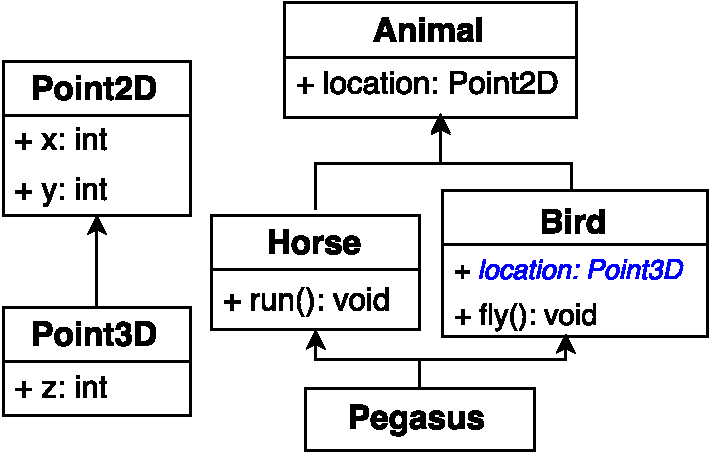
\includegraphics[height=4cm]{pdfs/PegasusDetail.pdf}\hspace{20pt} &
\begin{minipage}{7cm}
\vspace{-90pt}
\lstinputlisting[linerange=6-17]{../UseMixinLombok/src/pegasus/simple/java8/Main.java}% APPLY:linerange=PEGASUS_JAVA
%basicstyle=\ttfamily\scriptsize
\end{minipage}
\end{tabular}
\caption{The animal system (left: complete structure, right: code for simplified animal system).}\label{fig:pegasus}
\saveSpaceFig
\end{figure*}

This section illustrates how our programming style, supported by the
\mixinAnn{} annotation, enables powerful programming idioms based on multiple
inheritance and type refinements.  We propose a standard example:
\Q@Animal@s with a two-dimensional \Q@Point2D@ representing their
\Q@location@.  Some kinds of animals are \Q@Horses@ and \Q@Bird@s.
Birds can \Q@fly@, thus their locations need to be three-dimensional
\Q@Point3D@s (field type refinement).  Finally, we model \Q@Pegasus@
(one of the best-known creatures in Greek mythology) as a kind of
\Q@Animal@ with the skills of both \Q@Horse@s and \Q@Bird@s (multiple
inheritance). A simple class diagram illustrating the basic system is
given on the left side of Figure~\ref{fig:pegasus}.\footnote{Some
  research argues in favor of using subtyping for modeling taxonomies,
  other research argues against this practice, we do not wish to take
  sides in this argument, but to provide an engaging example.}

%\bruno{Should we provide a one sentence summary in the abstract of how much code
%is needed in Java (without Obj) vs the approach with CJ, for the Pegasus example?}
%\marco{Not in the abstract. But I think is good to have that number and to put in in the example section.
%I will set up the sentence and someone can compute the number.}

\subsection{Simple Multiple Inheritance with Default
  Methods}\label{sec:simple}

Before modelling the complete animal system, we  start with a
simplified version without locations. This version serves the purpose of illustrating how
Java 8 default methods can already model simple forms of multiple inheritance.
\texttt{Horse} and \texttt{Bird} are subtypes
of \texttt{Animal}, with methods \texttt{run()} and \texttt{fly()},
respectively. Pegasus can not only \emph{run} but also \emph{fly}! This is the
place where \emph{``multiple inheritance''} is needed, because
\texttt{Pegasus} needs to obtain \texttt{fly} and \texttt{run}
functionality from both \texttt{Horse} and \texttt{Bird}.
A first attempt to model the animal system in Java 8 is given on the right side
of Figure~\ref{fig:pegasus}.
Note that the implementations of the methods \texttt{run}
and \texttt{fly} are defined inside interfaces, using default
methods. Moreover, because interfaces support multiple interface
inheritance, the interface for \texttt{Pegasus} can inherit behaviour
from both \texttt{Horse} and \texttt{Bird}. Although Java interfaces
do not allow instance fields, no form of state is needed so far to
model the animal system.

\paragraph{Instantiation}
To use \texttt{Horse}, \texttt{Bird} and \texttt{Pegasus}, some
objects must be created first. A first problem with using
interfaces to model the animal system is simply that interfaces
cannot be directly instantiated. Classes, such as:

\lstinputlisting[linerange=21-23]{../UseMixinLombok/src/pegasus/simple/java8/Main.java}% APPLY:linerange=PEGASUS_INST

\noindent are needed for instantiation. Now a \texttt{Pegasus} animal can be created
using the class constructor:

\begin{lstlisting}
Pegasus p = new PegasusImpl();
\end{lstlisting}

\noindent There are some annoyances here. Firstly, the sole
purpose of the classes is to provide a way to instantiate
objects. Although (in this case) it takes only one line of code to
provide each of those classes, this code is essentially boilerplate
code, which does not add behavior to the system. Secondly,
the namespace gets filled with three additional types. For example,
both \texttt{Horse} and \texttt{HorseImpl} are needed: \texttt{Horse}
is needed because it needs to be an interface so that \texttt{Pegasus}
can use multiple inheritance; and \texttt{HorseImpl} is needed to
provide object instantiation.
Note that, for this very simple animal system, plain Java 8 anonymous
classes can be used to avoid these problems.  We could have simply
instantiated \texttt{Pegasus} using:

\begin{lstlisting}
Pegasus p = new Pegasus() {}; // anonymous class
\end{lstlisting}

\noindent However, as we shall see, once the system gets a little more
complicated, the code for instantiation quickly becomes more
complex and verbose (even with anonymous classes).

\subsection{Object Interfaces and Instantiation}

To model the animal system with object interfaces all that a user
needs to do is to add an \mixinAnn{} annotation to the \texttt{Horse},
\texttt{Bird}, and \texttt{Pegasus} interfaces:

\lstinputlisting[linerange=8-12]{../UseMixinLombok/src/pegasus/simple/lombok/Main.java}% APPLY:linerange=PEGASUS_LOMBOK
\noindent The effect of the annotations is that a static \emph{factory} method called
\texttt{of} is automatically added to the interfaces. With the
\texttt{of} method a \texttt{Pegasus} object is instantiated as follows:

\begin{lstlisting}
Pegasus p = Pegasus.of();
\end{lstlisting}

\noindent The \texttt{of} method provides an alternative to a
constructor, which is missing from interfaces. The following code
shows the code corresponding to the \texttt{Pegasus} interface
after the \mixinAnn{} annotation is processed:

\begin{lstlisting}
interface Pegasus extends Horse, Bird {
  // generated code not visible to users
  static Pegasus of() { return new Pegasus() {}; }
}
\end{lstlisting}

\noindent Note that the generated code is transparent to a user, who
only sees the original code with the \mixin annotation. Compared to the pure
Java solution in Section~\ref{sec:simple}, the solution using object interfaces
has the advantage of providing a direct mechanism for object
instantiation, which avoids adding boilerplate classes to the
namespace.

\subsection{Object Interfaces with State}

The animal system modeled so far is a simplified version of the
system presented in the left-side of Figure~\ref{fig:pegasus}.
The example is still not sufficient to appreciate the advantages of IB
programming.
Now we model the complete animal system where an \Q@Animal@ includes a \Q@location@
representing its position in space. We use 2D points to keep track of locations using coordinates.

\paragraph{\Q@Point2D@: simple immutable data with fields}
Here we will illustrate how points are modelled with interfaces. In IB
we do not talk about state directly. Instead, state is accessed and
manipulated using abstract methods.  The usual approach to model
points in Java is to use a class with fields for the coordinates.
In Classless Java interfaces are used instead:

\begin{lstlisting}
interface Point2D { int x(); int y(); }
\end{lstlisting}

\noindent The encoding over Java is now inconvenient: creating a new point object is cumbersome, even
with anonymous classes:

\begin{lstlisting}
Point2D p = new Point2D() {
  public int x() {return 4;}
  public int y() {return 2;}
}
\end{lstlisting}

\noindent However this cumbersome syntax is not required for every
object allocation. As programmers do, for ease or reuse, the boring
repetitive code can be encapsulated in a method. A generalization of the
\texttt{of} static factory method is appropriate in this case:
\begin{lstlisting}
interface Point2D { int x(); int y();
  static Point2D of(int x, int y) {
    return new Point2D() {
      public int x(){return x;}
      public int y(){return y;}
    };  }  }
\end{lstlisting}

\vspace{-5pt}
\paragraph{\Q@Point2D@ with object interfaces}
This obvious ``constructor'' code can be automatically generated by the \mixin
annotation.  By annotating the interface \Q@Point2D@, a variation of the shown
static method \texttt{of} will be generated, mimicking the functionality of a
simple-minded constructor. \mixin first looks at the abstract methods and detects
what the fields are, then generates an \Q@of@ method with one parameter for each
of them. That is, we can just write

\begin{lstlisting}
@Obj interface Point2D { int x(); int y(); }
\end{lstlisting}

\noindent More precisely, a field or factory parameter is generated for every
abstract method that takes no parameters (except for methods with special
names). An example of using \Q@Point2D@ is:
\begin{lstlisting}
Point2D p = Point2D.of(42,myPoint.y());
\end{lstlisting}
\noindent where we return a new point, using \Q@42@ as x-coordinate,
and taking all the other information (only \Q@y@ in this case) from
another point.

\paragraph{\texttt{with-} methods in object interfaces}
The pattern of creating a new object by reusing most information from an old
object is very common when programming with immutable
data-structures. As such, it is
supported by \mixin as \Q@with-@ methods. For example:
\begin{lstlisting}
@Obj interface Point2D {
    int x();    int y(); // getters
    // with- methods
    Point2D withX(int val);
    Point2D withY(int val);
}
\end{lstlisting}

\noindent Using \texttt{with-} methods, the point \texttt{p} can also be created
by:

\begin{lstlisting}
Point2D p = myPoint.withX(42);
\end{lstlisting}

\noindent If there is a large number of fields, \texttt{with-} methods
will save programmers from writing large amounts of tedious code that
simply copies field values.
\begin{comment}
is expanded by \mixin into\footnote{
Note how we actually generate a real field \Q@int x=_x;@.
This provides a more uniform translation that can work also for mutable data structures, where setters are required.
}

\begin{lstlisting}
interface Point2D { int x(); int y();
    static Point2D of(int _x, int _y){ return new Point2D(){
        int x=_x; int y=_y;
        public int x(){return x;}   public int y(){ return y; }
        Point2D withX(int val){ return Point2D.of(val,this.y()); }
        Point2D withY(int val){ return Point2D.of(this.x(),val); }
    }; }
  Point2D withX(int val);    Point2D withY(int val); }
\end{lstlisting}
\end{comment}
Moreover, if the programmer wants a different implementation, he may
provide an alternative implementation using \Q@default@ methods. For example:
\begin{lstlisting}
@Obj interface Point2D {
    int x(); int y();
    default Point2D withX(int val){ /*myCode*/ }
    default Point2D withY(int val){ /*myCode*/ } }
\end{lstlisting}

%\begin{comment}
%\marco{I re-enabled this code, I think is needed for understandability}
\noindent is expanded into
\begin{lstlisting}
interface Point2D {
    int x(); int y();
    default Point2D withX(int val){ /*myCode*/ }
    default Point2D withY(int val){ /*myCode*/ }
    static Point2D of(int _x, int _y){
      return new Point2D(){
        int x=_x;    int y=_y;
        public int x(){return x;}
        public int y(){return y;} }; } }
\end{lstlisting}

\noindent Only code for methods needing implementation is generated. Thus,
programmers can easily customize the behaviour for their special needs.
Also, since \mixin interfaces offer the \Q@of@ factory method, only interfaces where all the abstract methods
can be synthesized can be object interfaces. A non \mixin interface is like an abstract class in Java.
%\end{comment}

%Firstly, to model \texttt{Point2D} that has x-coordinate and y-coordinate by an
%interface, we immediately run into the problem of expressing the fields
%\texttt{x} and \texttt{y}.
%interfaces. Method \texttt{withX, withY} creates a new instance of
%\texttt{Point2D} with updated field \texttt{x,y}, respectively.

% Firstly, to model \texttt{Animal} by an interface, we immediately run into the
% problem of expressing the field \texttt{point}. Since in Java there is no way to
% define member fields inside interfaces, we propose to simulate fields by
% abstract methods inside interfaces:

%\lstinputlisting[linerange=42-48]{../UseMixinLombok/src/pegasus/TestAnimal.java}% APPLY:linerange=POINT2D

%\paragraph{Instantiation}
%In Java, to implement an interface like \texttt{Point2D}, a typical and trivial
%approach that programmers usually do is creating a class extending the interface
%and providing implementation for all methods inside. For example, this is the
%implementation for interface \texttt{Point2D}:

%\begin{lstlisting}
%class Point2DImpl implements Point2D {
%    private int _x;
%    private int _y;
%    public Point2DImpl(int x, int y) {
%        this._x = x;
%        this._y = y;
%    }
%    public int x() {
%        return _x;
%    }
%    public int y() {
%        return _y;
%    }
% %Your implementation of with is wrong
%    public Point2D withX(int x) {
%        x(x);
%        return this;
%    }
%    public void x(int x) {
%        _x = x;
%    }
%    public void y(int y) {
%        _y = y;
%    }
%    public Point2D withY(int y) {
%        y(y);
%        return this;
%    }
%}
%\end{lstlisting}
%
%\texttt{Point2DImpl} implements \texttt{Point2D} and provides a constructor with
%quite mechanical code. What's worse, the implementation in \texttt{Point2DImpl}
%may not be reused in a single inheritance language.

%
%\begin{lstlisting}
%  // inside interface Point2D
%  static Point of(int x, int y) {
%      return new Point() {
%          int _x = x;
%          int _y = y;
%          public int x() {
%            return _x;
%          }
%          public int y() {
%            return _y;
%          }
%          public Point2D withX(int x) {
%            x(x);
%            return this;
%          }
%          public void x(int x) {
%            _x = x;
%          }
%          public void y(int y) {
%            _y = y;
%          }
%          public Point2D withY(int y) {
%            y(y);
%            return this;
%          }
%    }
%  }
%\end{lstlisting}
%
%\lstinputlisting[linerange=-]{} % APPLY:linerange=POINT_OF

\paragraph{\Q@Animal@ and \Q@Horse@: simple mutable data with fields}
2D points are mathematical entities, thus we choose an immutable data structure to
model them. However animals are real world entities, and when an animal moves,
it is the \emph{same} animal with a different location. We model this with
mutable state.

%Now we proceed to define \texttt{Animal} with \texttt{point} ``member
%field''.
%%Not again, before we used only getters!
% Again, we model this member field with getter and setter methods:
\lstinputlisting[linerange=58-60]{../UseMixinLombok/src/pegasus/TestAnimal.java}% APPLY:linerange=ANIMAL

\noindent Here we declare an abstract getter and setter for the mutable ``field''
\Q@location@.  Without the \mixin annotation, there is no convenient way to
instantiate \texttt{Animal}.  For \texttt{Horse}, the \mixin annotation is used
and an implementation of \texttt{run()} is defined using a \Q@default@
method. The implementation of \texttt{run()} further illustrates the convenience of \texttt{with-} methods:

\lstinputlisting[linerange=64-67]{../UseMixinLombok/src/pegasus/TestAnimal.java}% APPLY:linerange=HORSE

\noindent Creating and using \texttt{Horse} is quite simple:

\lstinputlisting[linerange=10-12]{../UseMixinLombok/src/pegasus/TestAnimal.java}% APPLY:linerange=USINGHORSE

\noindent Note how the \texttt{of}, \texttt{withX} and
\texttt{location} methods (all generated automatically) provide a
basic interface for dealing with animals.

In summary, dealing with state (mutable or not) in object interfaces
relies on a notion of abstract state, and state is not directly
available to programmers. Instead programmers use methods, called
\emph{abstract state operations}, to interact with state.

% by method
%\texttt{run()}: method \texttt{withX} returns a new point object with field
%\texttt{x} updated by the argument to \texttt{withX}. Without these
%\texttt{with} methods, operations like \texttt{run()} would be much harder to define.

\subsection{Object Interfaces and Subtyping}
\Q@Bird@s are \Q@Animal@s, but while \Q@Animal@s only need 2D
locations, \Q@Bird@s need 3D locations. Therefore when the \texttt{Bird}
interface extends the \Q@Animal@ interface, the notion of points needs to
be \emph{refined}. Such kind of refinement is challenging
in typical \classbased approaches. Fortunately, with object interfaces,
we are able to provide a simple and effective solution.

\paragraph{Unsatisfactory \classbased solutions to field type refinement}
In Java if we want to define an animal class with a field we have a set of
unsatisfactory options in front of us:
\begin{itemize}
\item Define a \Q@Point3D@ field in \Q@Animal@: this is bad since all animals
  would require more than needed.
  %Also it requires the programmer to predict the future, or
  Also it requires adapting the old code to accommodate for new evolutions.

\item Define a \Q@Point2D@ field in \Q@Animal@ and define an extra \Q@int z@
  field in \Q@Bird@.  This solution is very ad-hoc, requiring to basically
  duplicate the difference between \Q@Point2D@ and \Q@Point3D@ inside \Q@Bird@.
  %Again, there are many reasons this would be bad,
  The most dramatic criticism is that it would not scale to a scenario when
  \Q@Bird@ and \Q@Point3D@ are from different programmers.

\item Redefine getters and setters in \Q@Bird@, always put \Q@Point3D@ objects
  in the field and cast the value out of the \Q@Point2D@ field to \Q@Point3D@
  when implementing the overridden getter.  This solution scales to the multiple
  programmers approach, but requires ugly casts and can be implemented in a
  wrong way leading to bugs.
\end{itemize}

We may be tempted to assume that a language extension is needed.
%Instead, with object interfaces, another approach is possible
Instead, the \emph{restriction} of (object) interfaces to have no
fields enlightens us that another approach is possible; often in programming languages ``freedom is slavery''.

\paragraph{Field type refinement with object interfaces}
Object interfaces address the challenge of type-refinement as follows:
\begin{itemize}
\item by \emph{covariant method overriding}, the return type of
  \texttt{location()} is refined to \texttt{Point3D};
\item by \emph{overloading}, a new setter for location is defined with a more
  precise type;
\item a \Q@default@ setter implementation with the old signature is provided.
\end{itemize}

Thus, with object interfaces, the code for the \Q@Bird@ interface is:

\lstinputlisting[linerange=71-80]{../UseMixinLombok/src/pegasus/TestAnimal.java}% APPLY:linerange=BIRD
%Interface \texttt{Point3D} extends \texttt{Point2D} with a new abstract method
%\texttt{int z()} (treated as a getter for member field \texttt{z}). Note that
%the return type of various methods (e.g. with- methods, getters) get refined
%either by covariant method overriding or automatically by our annotation
%processor. Besides \emph{with}, other methods (including \emph{clone},
%\emph{of}) also do type-refinements automatically.


\noindent From the type perspective, the key is the covariant method
overriding of \texttt{location()}. However, from the semantics
perspective the key is the implementation for the setter with the old
signature (\Q@location(Point2D)@). The key to the setter
implementation is a new type of \Q@with@ method, called
 a (functional) property updater.

\paragraph{\Q@Point3D@ and property updaters}
The \Q@Point3D@ interface is defined as follows:

\lstinputlisting[linerange=52-55]{../UseMixinLombok/src/pegasus/TestAnimal.java}% APPLY:linerange=POINT3D

\noindent \Q@Point3D@ includes a
\Q@with@ method, taking a \Q@Point2D@ as an argument.
Other wither methods (such as \Q@withX@) functionally update a field one at a time.  This can be
inefficient, and sometimes hard to maintain.  Often we want to update multiple
fields simultaneously, for example using another object as source.  Following
this idea, the method \Q@with(Point2D)@ is an example of a (functional)
property updater: it takes a certain type of object and returns a copy of the
current object where all the fields that match fields in the parameter
object are updated to the corresponding value in the parameter. The idea is that
the result should be like \Q@this@, but modified to be as similar as possible to the parameter.

With the new \Q@with@ method we may use the information for
\Q@z@ already stored in the object to forge an appropriate \Q@Point3D@
to store. Note how all the information about what fields sit in
\Q@Point3D@ and \Q@Point2D@ is properly encapsulated in the
\Q@with@ method, and is transparent to the implementer of \Q@Bird@.

Property updaters never break class invariants, since they
internally call operations that were already deemed
safe by the programmer. For example a list object
would not offer a setter for its \texttt{size} field (which should be kept hidden), thus
a property updater would not attempt to set it.

% To implement the old setter in a convenient way, \mixin supports one
% last type of operations: property updater \texttt{with}
% methods. Unlike the \texttt{withX} (where \texttt{X} stands for a
% field name) methods presented so far, property updaters take several
% fields at once, contained in an interface, and copy those fields into
% fields of another interface.

%Symmetrically, we could offer an imperative property updater that
%calls the setters instead of the withers.  \Q@Point3D set(Point2D
%val)@.

\begin{figure}
\saveSpaceFig
\lstinputlisting[linerange=89-115]{../UseMixinLombok/src/pegasus/TestAnimal.java}% APPLY:linerange=GENERATED_POINT3D
\caption{Generated boilerplate code.}
\label{fig:boilerplate}
\saveSpaceFig
\end{figure}

\paragraph{Generated boilerplate}
Just to give a feeling of how much mechanical code \mixin is generating, we show the
generated code for the \texttt{Point3D} in Figure~\ref{fig:boilerplate}.
%\marcoT{Overall, for the whole
%animals-with-locations, an @@@ lines code example,
%the generate/completed code is composed by
%@@@ lines.}
Writing such code by hand is error-prone. For
example a distracted programmer may swap the arguments of calls to
\Q@Point3D.of@.  Note how \Q@with-@ methods are automatically refined in their
return types, so that code like:

\begin{lstlisting}
Point3D p = Point3D.of(1,2,3); p = p.withX(42);
\end{lstlisting}

\noindent will be accepted. If the programmer wishes to suppress this behavior
and keep the signature as it was, it is sufficient to redefine the \Q@with-@
methods in the new interface repeating the old signature.  Again, the philosophy
is that if the programmer provides something directly, \mixin does not touch it.
The cast in \Q@with(Point2D)@ is trivially safe because of the \Q@instanceof@
test. The idea is that if the parameter is a subtype of the current exact type,
then we can just return the parameter, as something that is just ``more'' than
\Q@this@.


\begin{figure*}
\saveSpaceFig
\centering
\begin{tabular}{|l|l|l|l|}
\hline
& \textbf{Operation}  & \textbf{Example}                  & \textbf{Description } \\ \hline
\multirow{4}{*}{\parbox{2.5cm}{State operations (for a field \texttt{x})}} & \textbf{``fields''/getters}        &   \Q@int x()@                  & Retrieves value from field \texttt{x}.          \\ \cline{2-4}
& {\bf withers}        &   \Q@Point2D withX(int val)@                & Clones
object; updates field \texttt{x} to \texttt{val}.             \\ \cline{2-4}
& \textbf{setters}        & \Q@void x(int val)@ & Sets the field
\texttt{x} to a  new value \texttt{val}.        \\ \cline{2-4}
& \textbf{fluent setters}        & \Q@Point2D x(int val)@ &Sets the field
\texttt{x} to \texttt{val} and returns \texttt{\this}.           \\ \hline
\multirow{3}{*}{Other operations} &
\textbf{factory methods} &
%\begin{tabular}{l}
\Q@static Point2D of(int _x,int _y)@
%\end{tabular}
 & Factory method (generated).        \\
\cline{2-4}
& \textbf{functional updaters}        & \Q@Point3D with(Point2D val)@
& Update all matching fields in \texttt{val}.        \\ \hline
%\cline{2-4}
%& \textbf{imperative updaters}        & \Q@Point3D set(Point2D val)@ &
%Set all matching fields in \texttt{val}.        \\ \hline
\end{tabular}

\caption{Abstract state operations for a field \texttt{x}, together with other operations, supported by the \mixin
  annotation. }

\label{fig:abstractstate}

\end{figure*}

\paragraph{Summary of operations in Classless Java}
%Method bodies can only refer to other methods;
%Objects are (conceptually) closures and the state is
%composed by captured local variables.}
%Methods interacting with state are called \emph{abstract state operations}.
In summary, object interfaces provide support for
different types of abstract state operations: four field-based state
operations; and functional updaters. Furthermore object interfaces support
direct object instantiation via \texttt{of} factory methods.
Figure~\ref{fig:abstractstate} summarizes the six operations supported
by \mixin. The field-based abstract state operations are determined by
naming conventions and the types of the methods. Fluent setters are a variant of
conventional setters, and are discussed in more detail in Section~\ref{sec:dsls}.

\subsection{Advanced Multiple Inheritance}
Finally, defining \texttt{Pegasus} is as simple as we did in the simplified
(and stateless) version on the right of Figure~\ref{fig:pegasus}.
 Note how even the non-trivial pattern for field type refinement is
transparently composed, and \texttt{Pegasus} has a \Q@Point3D@
\Q@location@.%  This works because \Q@Horse@ do not perform
% any field type refinement, otherwise we may have to choose/create a
% common subtype in order for \texttt{Pegasus} to exists.

\lstinputlisting[linerange=84-84]{../UseMixinLombok/src/pegasus/TestAnimal.java}% APPLY:linerange=PEGASUS


\begin{comment}
\subsection{A Running Example: \texttt{Point}}
Suppose we want to create a point component that models the a point in space,
that has x-coordinate and y-coordinate. For example, if we create the
\texttt{Point} interface in Java, it would look like this:

\begin{lstlisting}
interface Point {
    int x();
    int y();
}
\end{lstlisting}

\texttt{Point} has two (conceptually) member fields \texttt{x} and \texttt{y},
representing the two coordinates of a point. Methods \texttt{int x()} and
\texttt{int y()} serve as \emph{getter} methods.
% Methods \texttt{void X(int X)} and \texttt{void Y(int Y)} serve as
% \emph{setter} methods. Method \texttt{Point withX(int X)} updates field
% \texttt{X} and returns \textbf{this}.

\subsection{Naive Implementation}
In Java, to implement an interface like \texttt{Point}, a typical and trivial
approach that programmers usually do is creating a class extending the interface
and providing implementation for all methods inside. For example, this is the
implementation for interface \texttt{Point}:

\lstinputlisting[linerange=-]{} % APPLY:linerange=POINTIMPL

\texttt{PointImpl} implements \texttt{Point} and provides a constructor with
quite mechanical code. What's worse, the implementation in \texttt{PointImpl}
may not be reused in a single inheritance language.

\subsection{The Classless Java Approach}
Instead of writing a whole another class to provide the implementation for
\texttt{Point}, we annotate on interface \texttt{Point} directly with \mixin:

\lstinputlisting[linerange=-]{} % APPLY:linerange=POINT

The \mixin annotation will generate a static method \texttt{of} inside
\texttt{Point}. The method \texttt{of} mimic the functionality of constructors,
it takes arguments same as constructors and return objects similar to
constructors. It makes use of Java anonymous classes and achieves the same
implementation as \texttt{PointImpl}.

With \CJ, we provide a Java annotation \mixin to provide default
implementations for various methods and a mechanism to instantiate
objects. \mixin annotation helps programmers to write less cumbersome code and
instantiate interfaces in Java.

\lstinputlisting[linerange=-]{} % APPLY:linerange=POINT_OF
\end{comment}


\begin{comment}
\subsection{More On \mixin}
Besides the benefit of freeing programmers from writing boilerplate code, our
\mixin annotation can also allow programs to mimic multiple inheritance in a
restricted form easily.

\lstinputlisting[linerange=42-48]{../UseMixinLombok/src/pegasus/TestAnimal.java}% APPLY:linerange=POINT2D

\lstinputlisting[linerange=52-55]{../UseMixinLombok/src/pegasus/TestAnimal.java}% APPLY:linerange=POINT3D

\lstinputlisting[linerange=58-60]{../UseMixinLombok/src/pegasus/TestAnimal.java}% APPLY:linerange=ANIMAL

\lstinputlisting[linerange=64-67]{../UseMixinLombok/src/pegasus/TestAnimal.java}% APPLY:linerange=HORSE

\lstinputlisting[linerange=71-80]{../UseMixinLombok/src/pegasus/TestAnimal.java}% APPLY:linerange=BIRD

\lstinputlisting[linerange=84-84]{../UseMixinLombok/src/pegasus/TestAnimal.java}% APPLY:linerange=PEGASUS

Interface \texttt{Point3D} extends \texttt{Point/Point2D} with a new abstract
method \texttt{int z()} (treated as a getter for member field
\texttt{z}). Interface \texttt{Horse} shows the usage and advantage of
\emph{with} methods by method \texttt{run()}: method \texttt{withX} returns a
new point object with field \texttt{x} updated by the argument to
\texttt{withX}. Without these \texttt{with} methods, operations like
\texttt{run()} would be much harder to define. Note that the return type of
various methods get refined automatically by our annotation processor. Besides
\emph{with}, other methods (including \emph{clone}, \emph{of}) also do
type-refinements automatically.

The \emph{``multiple inheritance''} case appears at interface
\texttt{Pegasus}. Pegasuses can not only \emph{run} but also \emph{fly}!
Interface \texttt{Pegasus} obtains \texttt{fly} and \texttt{run} functionality
through interface \texttt{Horse} and \texttt{Bird}. Using \mixin annotation,
actually there is no code that programmers have to write at all. The idea of using
default methods inside interfaces was proposed in ~\cite{}. It enables us to do
multiple inheritance, which otherwise is hard to do in Java-like languages that
do not support multiple inheritance, easily.
\end{comment}



\section{Bridging between IB and CB in Java}\label{sec:imp}


%\footnote{ Rewriting libraries and
%  application in this language/model would result in more reusable
%  libraries, but it would be a taunting task.}
Creating a new language/extension would be an
elegant way to illustrate the point of IB. However,
significant amounts of engineering would be needed to build a practical
language and achieve a similar level of integration and tool support
as Java. To be practical, %To have an approach that can both illustrate IB programming and be practical, 
we have instead implemented
\mixin as an annotation in Java 8, and a \emph{compilation agent}.
That is, the Classless Java style of programming
is supported by library.

Disciplined use of Classless Java (avoiding class
declarations as done in Section~\ref{sec:ep}) illustrates what \emph{pure} IB is like.
However, using \mixin, CB and IB programming can be mixed together,
harvesting the practical convenience of using existing Java libraries, the full
Java language, and IDE support.
The key to our implementation is compilation agents, which
 allows us to rewrite the Java AST just
before compilation. We discuss advantages and limitations of our approach.

\subsection{Compilation Agents}
Java supports compilation agents, where Java libraries can interact with the Java compilation process,
acting as a man in the middle between the
generation of AST and bytecode.

This process is facilitated by frameworks like Lombok~\cite{lombok}:
a Java library that aims at reducing Java boilerplate code via 
annotations. \mixin was created using Lombok.
Figure~\ref{fig:lombok}~\cite{neildo2011blog} illustrates the flow of
the \mixin annotation.
First Java source code is parsed into an abstract syntax tree (AST).
The AST is then captured by Lombok:
each annotated node is passed to
the corresponding (Eclipse or Javac) handler. The handler is
free to modify the information of the annotated node, or even inject new nodes (like methods, inner classes,
etc). Finally, the Java compiler works on the modified AST to generate bytecode.
%Note how during the compilation,
%no source code is changed, and no new source/temporary files are created.


%There are a number of annotations provided by the
%original Lombok, including \Q:@Getter:, \Q:@Setter:,
%\Q:@ToString: for generating getters, setters and \QM{toString}
%methods, respectively.  Furthermore, Lombok provides a number of
%interfaces for users to create custom transformations, as extensions
%to the original framework.
%A transformation is based on a handler, which acts on the AST for the
%annotated node and returns a modified AST for analysis and
%generation afterwards. Such a handler can either be a Javac handler or
%an Eclipse handler.

\begin{figure}[t]
\saveSpaceFig
\centering
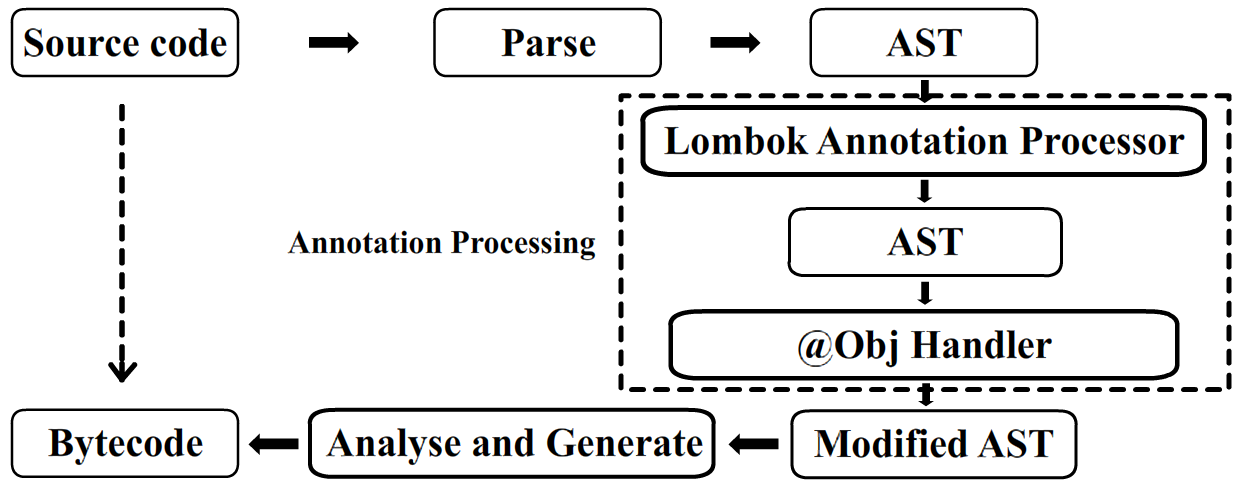
\includegraphics[width=3in]{pdfs/lombok3.png}
\caption{The flow chart of \mixin annotation processing.
}
\label{fig:lombok}
\saveSpaceFig
\end{figure}


\paragraph{Advantages of Lombok}
The Lombok compilation agent has advantages over 
pre-processors or other Java annotation processors.
Lombok offers in Java an expressive power similar to that of Scala/Lisp macros,
except, for the syntactic convenience of quote/unquote templating. Compilation
agents act modularly on each compilation unit, applying transformations to one 
annotated class/interface at a time. This allows library code to be reused
without the need of being reprocessed and recompiled, making our
approach 100\% compatible with existing Java libraries. 
In Eclipse, the processing is 
performed transparently and the information of the interface from
compilation is captured in the ``Outline'' window as shown in Figure~\ref{fig:screenshot}..
This includes all the methods inside the interface as well as the generated ones.

\begin{figure*}[t]
\saveSpaceFig
\saveSpaceFig
\centering
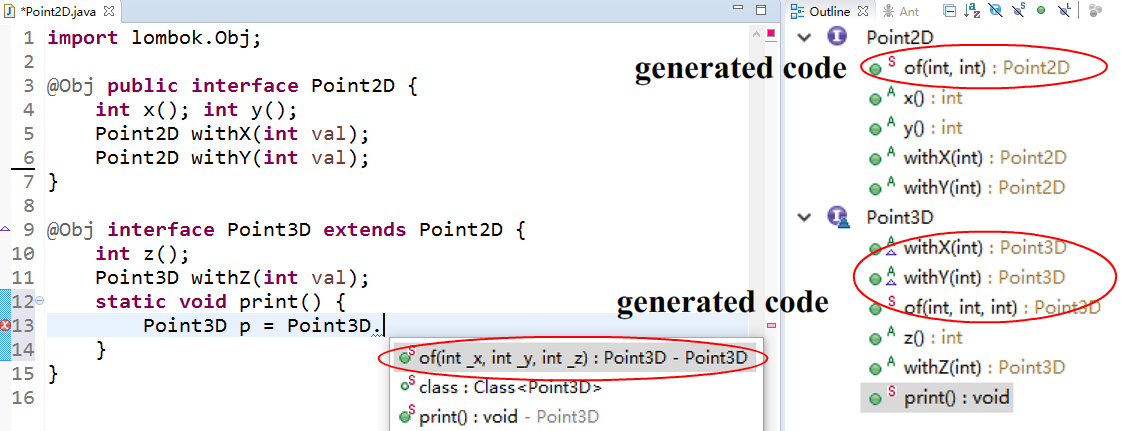
\includegraphics[width=4.5in]{pdfs/screenshot4.png}
\caption{Generated methods shown in the Outline window of Eclipse and auto-completion.}
\label{fig:screenshot}
\saveSpaceFig
\end{figure*}

\begin{comment}
\paragraph{Direct modification of the AST}
Lombok alters the generation process of the class files,
by directly modifying the AST. Neither the source code is modified nor
new Java files are generated. Moreover, and probably more importantly,
Lombok supports generation of code \emph{inside} a class/interface,
which conventional Java annotation processors do not support. For
example, the standard \texttt{javax.annotation} processor, which is part of the
Java platform, only allows generation of \emph{new code}, and the
new code has to be written in \emph{new files}. Modification and/or
reinterpretation of existing code are not supported. 

\paragraph{Modularity}
While general preprocessing acts across module boundaries, compilation
agents act modularly on each class/compilation unit. It makes sense to
apply the transformations to one class/interface at a time, and only to
annotated classes/interfaces. This allows library code to be reused
without the need of being reprocessed and recompiled, making our
approach 100\% compatible with existing Java libraries, which can be
used and extended normally. Of course, Java libraries can also receive
and use instances of object interfaces as normal objects.

\paragraph{Tool support}
Features written in Lombok integrate and are supported directly in the
language, and are often also supported by (most) tools.  For example in Eclipse, the processing is
performed transparently and the information of the interface from
compilation is captured in the ``Outline'' window.
This includes all
the methods inside the interface as well as the generated ones.
In Figure~\ref{fig:screenshot},
\mixin generates an \Q@of@ method in \Q@Point2D@, and \Q@of@, \Q@withX@, \Q@withY@ methods in \Q@Point3D@.
These methods are also visible to users, showing their types and modifiers in Outline window.
Moreover, as a useful IDE feature, the auto-completion also works for these newly generated methods.

\paragraph{Clarity against obfuscation}
Preprocessors bring great power, which can easily be misused producing
code particularly hard to understand. Thus code quality and maintainability are reduced.
Compilation agents start from Java syntax, but they can reinterpret it.
Preserving the syntax avoids syntactic conflicts, and allows many
tools to work transparently.
\end{comment}

\subsection{\mixin AST Reinterpretation}

Of course, careless reinterpretation of the AST could still be
surprising for badly designed rewritings.  \mixin reinterprets
the syntax with the sole goal of \emph{enhancing and completing code}:
we satisfy the behaviour of abstract methods; add method
implementations; and refine return types.  We consider this to be
quite easy to follow and reason about, since it is similar to what
happens in normal inheritance.  Refactoring operations like renaming
and moving should work transparently in conjunction with our
annotation, since they rely on the overall type structure of the
class, which we do not arbitrarily modify but just complete.

Thus, in addition to the advantages of Lombok, Classless Java offers
some more advantages with respect to arbitrary (compilation agent driven) AST rewriting.

%\marco{The section No reuse of the type system
%is controversial.
%We do need to repeat the type checking, plus we aim to make untypable stuff well typed
%(for example anyone using the of method would not be well typed before).}
%\item \textbf{No reuse of the type system.}
%As we mentioned above, badly designed rewritings can arise from the great power of Lombok. A simple piece of source code
%\begin{lstlisting}
%interface M { int m(); }
%\end{lstlisting}
%can be reinterpreted as
%\begin{lstlisting}
%interface M { void m(String s); }
%\end{lstlisting}
%in which case the type of method \Q@m@ is changed. Our \mixin annotation does not introduce this kind of rewritings,
%and hence the type system is reused. Moreover, Lombok can also modify unbounded types, which is easy to understand,
%for instance, the following code
%\begin{lstlisting}
%interface M { T m(); } // T is unbounded
%\end{lstlisting}
%is transformed into
%\begin{lstlisting}
%interface M { int m(); } // No error message
%\end{lstlisting}
%in which case the user will see the unbounded type in source code, but without error message from the compilation, since
%Lombok has modified the return type of \Q@m@. However, our \mixin annotation can still keep such errors and warnings.


%\item \textbf{Lack of reuse.}  %not sure here... I think most preprocessors support decent reuse, even the C one
%Reusability is yet another concern in using preprocessors.
% In Lombok, implementations of features are
%encapsulated in various annotation handlers,
% in which case some behaviours are allowed to reuse the code by invoking methods
%in other handlers, where tedious replicated code is avoided.



\paragraph{Syntax and type errors}
Some preprocessors (like the C one) can produce syntactically invalid code.
Lombok ensures only syntactically valid code is produced. %; however, type errors can appear.
Classless Java additionally guarantees that no type errors are introduced
in generated code and client code. We discuss these two guarantees in
more detail next:

\begin{itemize}

\item{\bf Self coherence}: the generated code itself is well-typed. That is,
  type errors are not present in code the user has not written (for
  example \texttt{of} methods in Figure~\ref{fig:screenshot}).
In our case, it means that either \mixin{} produces (in a controlled way) an
understandable error or the interface can be successfully annotated and the generated code is well-typed.

\item{\bf Client coherence}: all the client code (for example method calls)
  that is well-typed before code generation is also well-typed after the generation.
The annotation just adds more behaviour without removing any functionality.

\end{itemize}

\paragraph{Heir coherence} Another form of guarantee that could be
useful in AST rewriting is heir coherence. That is, interfaces
(and in general classes) inheriting the instrumented code are
well-typed if they were well-typed without the instrumentation.
In a strict sense, our rewriting \emph{does not} guarantee heir coherence.  The reason
is that this would forbid adding any (default or abstract) method to
the annotated interfaces, or even doing type refinement. Indeed consider
the following:

\begin{lstlisting}
interface A { int x(); A withX(int x); }
@Obj interface B extends A {}
interface C extends B { A withX(int x); }
\end{lstlisting}

\noindent This code is correct before the translation, but \mixin would  generate in \Q@B@  a method ``\Q@B withX(int x);@''.
This would break \Q@C@.
Similarly, an expression of the form ``\Q@new B(){.. A withX(int x){..}}@''
would be correct before translation, but ill-typed after the translation.

Our automatic type refinement is a useful and convenient feature, but
not transparent to the heirs of the annotated interface.  They need to
be aware of the annotation semantics and provide the right type while
refining methods. To support heir coherence, we would need
to give up automatic type refinement, which is an essential part of IB programming.
However, the reader should note that Java libraries almost always break heir
coherence during evolution and still claim backward compatibility (false in
theory but statistically true in practice). In practice, adding any method to any
non-final class of a Java library is enough to break heir
coherence.  We think return type refinement breaks heir coherence ``less" than normal library evolution, and
if no automatic type-refinements are needed, then \mixin can claim a
form of heir coherence.
%Section~\ref{sec:translation} 
We provide a formal definition for our safety claims here~\footnote{See url?? Section B}.

\subsection{Limitations}
Our prototype implementation has certain limitations:
\begin{itemize}
\item Lombok allows writing handlers for either javac or ejc(Eclipse's own compiler).
Our current implementation only realizes ejc version. The implementation for
  the \texttt{javac} version is still missing.
\item Simple generics is supported:
type parameters can be used, but generic
method typing %is neither formalized in this paper nor 
not explicitly checked by \mixin, but simply delegated to the Java compiler.
\item
Lombok offers only limited/experimental support for separate compilation, that is
to access information of code defined in different files.
Limited by Lombok, \mixin 
%In the same spirit, we have a mature \mixin annotation, which
%does not support separate compilation yet: it 
requires that all
  related interfaces have to appear in a single Java file.
Reusing the logic inside the experimental Lombok annotation \lstinline{@Delegate},
we also offer a less polished annotation supporting
separate compilation for files in the same package.
%  has the same behavior as \mixin. A limitation is
%  that users need to put references to the super types
% of the annotated type together with the annotation, for instance,
%  \lstinline{@Delegate(types = Point2D.class)}.
%   Another limitation is the methods generated by \lstinline{@Delegate} will
%  not be visible in the Outline window, but they can still be auto-completed in Eclipse.
\end{itemize}


%\paragraph{Lombok does language tuning}
%We consider Lombok to be the most developed example of language
%tuning.  While the authors of Lombok do not introduce a specific term
%for what they are doing, their slogan \emph{``Spice up your java''}
%seems to be in line with the philosophy of language tuning. Some
%other examples of language tuning in Lombok include the \Q@val@ type,
%similar to \Q@auto@ in C\# or C++04.  Another library doing language
%tuning is CoFoJa~\cite{cofoja}, where annotations are used to insert
%pre-post conditions in generated bytecode.



\section{Interaction of Interface Methods with Interface Composition}
Before formalizing Classless Java and object interfaces, it is helpful
to informally discuss the behaviour of methods in Java 8
interfaces. In particular it is useful to understand how Java 8
interfaces differ from conventional trait models.

%We show several interesting cases
%and summarize compilation result of method composition into 3 categories:
%conflict error, accepted (both abstract) and conservative error. Meanwhile we
%also show different composition handling mechanism among traits, javac and ECJ.

\subsection{Methods in Java 8 Interfaces}
In Java 8 interfaces there are three types of methods: abstract, default, and
static methods.

\paragraph{Static methods} are handled in a very clean way: they are visible only in
  the interface in which they are explicitly defined. This means the following code
  is ill-typed.
\begin{lstlisting}
interface A0 { static int m(){return 1;} }
interface B0 extends A0 {}
... B0.m()//ill typed
\end{lstlisting}
This is different from the way static methods are handled in classes. Here
static methods have simply no interaction with interface
composition (\Q@extends@ or \Q@implements@).

\paragraph{Abstract method} composition is accepted when there exists a most specific one.
  For example, here method \texttt{Integer m()} from \texttt{B1} is visible in \Q@C1@.
\begin{lstlisting}
interface A1 { Object m(); }
interface B1 { Integer m();}
interface C1 extends A1,B1 {} //accepted
\end{lstlisting}

\paragraph{Default methods} conflict with any other default or abstract method. For
  example the following code is rejected due to method conflicts.
\begin{lstlisting}
interface A2 { default int m() {return 1;}}
interface B2 { int m(); }
interface C2 { default int m() {return 2;}}
interface D2 extends A2,B2 {} //rejected due to conflicting methods
interface E2 extends A2,C2 {} //rejected due to conflicting methods
\end{lstlisting}
Note how this is different from what happens in most trait models, where \Q@D2@
would be accepted, and the implementation in \Q@A2@ would be part of the
behaviour of \Q@D2@.

\paragraph{Resolving conflicts:}
A method in the current interface wins over any method in its
super-interfaces, provided that the method
is the most specific one. This method also overrides conflict due to
inheritance. For example, the following code is accepted, but would be rejected
(see before) if the method \Q@m@ was not redefined in \texttt{D3} and
\texttt{E3}.
\begin{lstlisting}
interface D3 extends A2,B2 { int m(); } //accepted
interface E3 extends A2,C2 { default int m(){return 42;} } //accepted
\end{lstlisting}

\subsection{Classifying Outcomes of Interface Composition}
%When interfaces are composed and methods with the same name (and
%signature) exist, there are 3 possible outcomes.
%
We now try to classify possible outcomes for composition of methods with the same name (and
signature).
We will use the following (correct) declarations:
\begin{lstlisting}
interface A1{T m(); }
interface A2 extends A1{default T m(){ ... } }
interface A3 extends A2{T m(); }

interface B1{default T m(){ ... } }
interface B2 extends B1{T m(); }
interface B3 extends B2{default T m(){ ... } }
\end{lstlisting}

\noindent
What happens if a new interface \Q@M@ extends one \Q@A@${}_i$ and one
\Q@B@${}_j$?\\*
% Nine representative cases are shown next:\\*
\noindent
\begin{tabular}{|l|l|l|l|}
\hline
\textbf{M extends} & \textbf{A1}                  & \textbf{A2} & \textbf{A3} \\ \hline
\textbf{B1}        & conservative error                        & conflict error      & conservative error       \\ \hline
\textbf{B2}        & both abstract, accepted                        & conservative error       & both abstract, accepted       \\ \hline
\textbf{B3}        & \textbf{conservative error} &conflict  error       & conservative error      \\ \hline
\end{tabular}
\\*
%We try to classify the results in the table:
\begin{itemize}
\item \textbf{conflict error} happens when the methods from both interfaces are implemented, which is also an error in most trait models.
\item \textbf{both abstract, accepted} happens when the methods from both interfaces are abstract, which is also considered correct in all
  trait models.
\item \textbf{conservative error} happens when only one method is implemented
  (leaving another one abstract), which is different from what we would expect in
  a trait model, but is coherent with the conservative idea that a method
  defined in an interface should not silently satisfy a method in another one.
\end{itemize}

\paragraph{A bug:} During our experimentation, we found a bug in ECJ (Eclipse compiler for Java):
the case \textbf{M} extending \textbf{B3} and \textbf{A1} is accepted by
ECJ4.5.1 and rejected by javac.  By email communication with Brian Goetz
(leading Java 8 designer) we have confirmed that the expected behaviour is
rejection, hence this is a bug in ECJ. This bug was also reported by
  others and is fixed in the ECJ developer branch, but not released as a stable
  version yet.
%Table~\ref{table:javabug} shows the method overriding bug in Java. In the
%example, there are 6 interfaces \texttt{A1,A2,A3,B1,B2,B3} with methods all
%named as \texttt{m} which are either abstract or default methods. If we define a
%new interface \texttt{M} that extends two of these interfaces, then the method
%overriding result is shown in the table. For example, row2 col2 means \texttt{M
%  extends A1,B1}. The result is \texttt{ERROR} because the abstract method
%\texttt{T m();} in \texttt{A1} conflicts with the method \texttt{default T m()
%  {...}} in \texttt{B1}. Readers may also figure out other extending cases by
%following this way of interpretation.

% The interesting case in row4 col2 where
%Indeed, to be coherent with the idea of \textbf{conservative error}, the case should not be accepted.
%We do not see how this should behave differently from \textbf{B1},\textbf{A1}, and \textbf{B3},\textbf{A3}.
%We fear that the only retro-compatible fix for this strange behaviour is to accept all the cases of \textbf{conservative error} in a future version of Java.
%the experimental result is \texttt{B3.m}. Because if we think consistently, this

%\lstinputlisting[linerange=4-9]{../UseMixinLombok/src/methodshadowing/test5/Test5.java} % APPLY:linerange=JAVABUG

%In our approach, we choose to not model this strange behaviour (a bug?).
%Our auxiliary function $\mBody(\m,\C)$ enforce the \textbf{conservative error} strategy.
%The rest of our formalization is parametric with the definition of $\mBody(\m,\C)$, thus if Java changes its resolution strategy to a more permissive one, only minor adaptations in $\mBody(\m,\C)$ would be needed.

\section{Formal Semantics}\label{sec:formal}

This section presents a formalization of Classless Java: a minimal
FeatherweightJava-like calculus which models the essence of Java
interfaces with default methods. This formalization is used in
Section~\ref{sec:translation} to define the semantics of object interfaces.


\begin{figure}[t]
\begin{grammar}
\production{
\e
}{
  \x\mid\MCall\e\m\es\mid\MCall{\C}\m\es\mid\MCall{\C\QM{.super}}\m\es\mid\x\QM=\e\QM;\e'\mid\obj
  }{expressions}\\
\production{
\obj
}{
\QM{new}\ \C\oR\cR\oC\fields\
\mh_1\oC\QM{return}\ \e_1\QM{;}\!\cC
\ldots
\mh_n\oC\QM{return}\ \e_n\QM{;}\!\cC
\cC
  }{object creation}\\
\production{\field}{\T\ \f \QM= \x\QM;}{field declaration}\\
\production{
\II
}{
 \ann\ \QM{interface}\ \C\ \QM{extends}\ \Cs\ \oC \methods\ \cC
  }{interface declaration}\\
\production{
\method
}{
 \QM{static}\ \mh\ \oC\QM{return}\ \e\QM{;}\!\cC
\mid
\QM{default}\ \mh\ \oC\QM{return}\ \e\QM{;}\cC
\mid
\mh\QM{;}
  }{method declaration}\\
\production{
\mh
}{
 \T_0\ \m\ \oR\T_1\ \x_1\ldots\T_n\ \x_n\cR
  }{method header}\\
\production{
\ann
}{
  \mixinAnn|\emptyset
  }{annotations}\\
\production{\Gamma}{
\x_1{:}\C_1\ldots\x_n{:}\C_n
}{environment}
\end{grammar}
\caption{Grammar of Classless Java}
\label{Grammar}
\end{figure}

\subsection{Syntax}

Figure~\ref{Grammar} shows the syntax of Classless Java.
The syntax formalizes a minimal
subset of Java 8, focusing on interfaces, default methods and object
creation literals.  There is no syntax for classes.
To help readability we use many metavariables to represent identifiers: $C,x,f$ and $m$; however they all map to a single set of identifiers as in Java.  Expressions
consist of conventional constructs such as variables ($\x$), method
calls ($\e\QM.\m\QM(\es)$) and static method calls
($\C\QM.\m\QM(\es)$). For simplicity the degenerate case of calling a
static method over the $\this$ receiver is not considered.  A more
interesting type of expressions is super calls
($\C\QM{.super.}\m\QM(\es)$), whose semantics is to call the (non-static) method $\m$ over the $\this$ receiver, but statically
dispatching to the version of the method as visible in the interface
$\C$. A simple form of field updates ($\x\QM=\e\QM;\e'$) is also
modelled. In the syntax of field updates $\x$ is expected to be a
field name. After updating the field $\x$ using the value of $\e$, the
expression $\e'$ is executed. To blend the statement based nature of
Java and the expression based nature of our language, we consider a
method body of the form \Q@return@ $\x\QM=\e\QM;\e'$ to represent
$\x\QM=\e\QM;\QM{return}\ \e'$ in Java.  Finally, there is an object
initialization expression from an interface $\C$, where (for
simplicity) all the fields are initialized with a variable present in
scope.
To  be fully compatible with Java, the concrete syntax for an interface
  declaration with empty supertype list  would also
  omit the \Q@extends@ keyword.
% The single
%non-Java 8 piece of syntax is the \mixin annotation, which is the only
%one interesting piece of syntax in this article.
%??? how is @Mixin not java8? in the sense that is java5?
  Following standard
practise, we consider a global Interface Table (\metaVar{IT}) mapping
from interface names $\C$ to interface declarations $\II$.

The environment $\Gamma$ is a mapping from variables to types.  As
usual, we allow a functional notation for $\Gamma$ to do variable
lookup.  Moreover, to help us define auxiliary functions, a functional
notation is also allowed for a set of methods $\methods$, using the
method name $\m$ as a key.  That is, we define $\methods(\m)=\method$
iff there is a unique $\method\in\methods$ whose name is $\m$.  For
convenience, we define $\methods(\m)=\none$ otherwise; moreover
$\m\in\dom(\methods)\ \miff\ \methods(\m)=\method$.
For simplicity, we do not model overloading, thus for an interface to be well formed its methods must be uniquely identified by their names.

\subsection{Typing}

Typing statement $\Gamma \vdash \e\in\C$ reads ``in the environment
$\Gamma$, expression $\e$ has type $\C$.''.
Before discussing the typing rules we discuss some of the used notation.
As a shortcut, we write
$\Gamma \vdash \e\in\C<:\C'$ instead of $\Gamma \vdash \e\in\C$ and
$\C<:\C'$.

We omit the definition of
the usual traditional subtyping relation between interfaces, that is the transitive and reflexive closure of the declared \Q@extends@ relation.
The auxiliary notation $\Gamma^\mh$ trivially
extracts the environment from a method header, by collecting the all types
and names of the method parameters.  The
notation $\m^\mh$ and $\C^\mh$ denotes respectivelly, extracting the
method name and the return type from a method header. $\mBody(\m,\C)$,
defined in Section~\ref{sec:auxiliary},
returns the full method declaration as seen by $\C$, that is the
method $\m$ can be declared in $\C$ or inherited from another
interface.
$\textsf{mtype}(\m,\C)$ and $\textsf{mtypeS}(\m,\C)$ return the type
signature from a method (using $\mBody(\m,\C)$ internally).
$\textsf{mtype}(\m,\C)$ is defined only for non static methods, while
$\textsf{mtypeS}(\m,\C)$ only for static ones. We use $\dom(\C)$ to
denote the set of methods that are defined for type $\C$, that is:
$\m\in\dom(\C)\ \miff \ \mBody(\m,\C)=\method$.

\begin{figure}[t]
$
\begin{array}{l}

%% T-Invk
\inferrule[(T-Invk)]{
 \Gamma \vdash \e \in \C_0 \\\\
\forall i\in 1..n\ \ \Gamma \vdash \e_i \in \_<:\C_i \\\\
  \textsf{mtype}(\m,\C_0) \!=\! \C_1\ldots\C_n \!\!\to\! \C
%\textsf{mmodifier}(\m,\C) \neq \textbf{static}
 }{
 \Gamma \vdash \e\QM.\m\QM(\e_1\ldots\e_n\QM) \in \C }
\quad\quad

%%T-StaticInvk
\inferrule[(T-StaticInvk)]{
\forall i\in 1..n\  \ \Gamma \vdash \e_i\in \_<:\C_i \\\\
\textsf{mtypeS}(\m,\C_0) \!=\! \C_1\ldots\C_n \!\to\! \C
%\textsf{mmodifier}(\m,\C) = \textbf{static}
}{
\Gamma \vdash \C_0\QM.\m\QM(\e_1\ldots\e_n\QM) \in \C}
\quad\quad

%%T-SuperInvk
\inferrule[(T-SuperInvk)]{
\Gamma(\this) <: \C_0 \\\\
\forall i\in 1..n\ \ \Gamma \vdash \e_i\in \_<:\C_i \\\\
  \textsf{mtype}(\m,\C_0) \!=\! \C_1\ldots\C_n \!\!\to\! \C
%\textsf{mmodifier}(\m,\C_0) \neq \textbf{static} \\\\
}{\Gamma \vdash \C_0\QM.\QM{super}\QM.\m\QM(\e_1\ldots\e_n\QM) \in \C}


%%T-Var
\\[5ex]
\inferrule[(T-Var)]{
\Gamma(\x)=\C
}{
\Gamma \vdash \x \in\C}
\quad\quad

%%T-Obj
\inferrule[(T-Obj)]{
\forall i\in 1..k\ \ \Gamma(\x_i)\subtype\T_i\\\\
\forall i\in 1..n\ \
%\Gamma_i
\Gamma,\f_1{:}\T_1,\ldots,\f_k{:}\T_k,\,\QM{this}{:}\C,\Gamma^{\mh_i}
\vdash\e_i\in \_\subtype\C^{\mh_i}\\\\
\sigvalid(\mh_1\ldots\mh_n,I)\quad\quad\quad\quad
%\forall i\in 1..n\ \mh_i\subtype\mBody(\m^{\mh_i},\C)\\\\
\alldefined(\mh_1\ldots\mh_n,I)
%\forall\m\mbox{ such that }
%\mBody(\m,\C)=\mh\QM; \exists i\in 1..n\ \m^{\mh_i}=\m
%\forall i\in 1\ldots n\ \Gamma_i=\Gamma,\f_1{:}\T_1,\ldots,\f_k{:}\T_k,\,\QM{this}{:}\C,\Gamma^{\mh_i}
}{
\Gamma \vdash\QM{new}\ \C\oR\cR\oC\T_1\ \f_1\QM=\x_1\QM;\ldots\T_k\ \f_k\QM=\x_k\QM;\
\mh_1\oC\QM{return}\ \e_1\QM{;}\!\cC
\ldots
\mh_n\oC\QM{return}\ \e_n\QM{;}\!\cC
\cC
\in\C
}
\\[5ex]



%%T-update
\quad
\inferrule[(T-update)]{
\Gamma \vdash \e\in\_<:\Gamma(\x)\\\\
\Gamma \vdash \e'\in\C
}{
\Gamma \vdash \x\QM=\e\QM;\e'\in\C }
\quad\quad\quad

%%T-Intf
 \inferrule[(T-Intf)]{
IT(\C) = \ann\ \QM{interface}\ \C\ \QM{extends}\ \C_1\ldots\C_n \
\oC\methods\ \cC\\\\
 \forall \QM{default}\ \mh\ \oC\QM{return}\ \e\QM;\cC \in \methods,
\ \ \Gamma^{\mh},\,\QM{this}{:}\C\vdash\e\in \_\subtype\C^{\mh} \\\\
 \forall \QM{static}\ \mh\ \oC\QM{return}\ \e\QM;\cC \in \methods,
\ \ \Gamma^{\mh}\vdash\e\in \_\subtype\C^{\mh} \\\\
\dom(\C)=\dom(\C_1)\cup\ldots\cup\dom(\C_n)\cup\dom(\methods)
 }{
\C \text{ OK}
}
\end{array}$
\caption{CJ Typing}
\label{ET}
\end{figure}

In Figure~\ref{ET} we show the typing rules.  We discuss the
most interesting rules, that is \rn{t-Obj} and \rn{t-Intf}. Rule
\rn{t-Obj} is the most complex typing rule. Firstly, we need to
ensure that all field initializations are type correct, by looking up the type of
each variable assigned to a field in the typing environment and verifying that such type is a
subtype of the field type. Secondly, we check that all method bodies are
well-typed. To do this the environment used to check the method body
needs to be extended appropriately: we add all fields and their types;
add $\this:I$; and add the arguments (and types) of the respective
method.
Now we need to check if the object is a valid extension for that specific interface.
This can be logically divided into two steps.
First  we check that all method headers are valid
with respect to the corresponding method already present in $\C$:

\noindent$\begin{array}{l}
\InTextDef{10em}{\sigvalid(\mh_1\ldots\mh_n,I)
}{
\forall i\in 1..n\ \ \mh_i\QM;\subtype\mBody(\m^{\mh_i},\C)
}
\end{array}$

\noindent Here we require that for all newly declared methods, there is a method
with the same name defined in the interface $\C$, and that such method is a
supertype of the newly introduced one. We define subtyping between methods in a
general form that will also be useful later.

\noindent$\begin{array}{l}
\InTextDef{18em}{
\T\ \m\oR\T_1\x_1\ldots \T_n\x_n\cR\QM; \subtype \T' \m\oR\T_1\x_1'\ldots\T_n\x_n'\cR\QM;
}{
\T\subtype \T'
}\\
\InTextDef{18em}{\method \subtype
\QM{default}\ \mh\,\mbox{\Q@\{return \_;\}@}
}{
\method\subtype\mh\QM;
}\\
\InTextDef{18em}{\QM{default}\ \mh\,\mbox{\Q@\{return \_;\}@}\subtype\method
}{
\mh\QM;\subtype\method
}\\
\end{array}$

\noindent We allow return type specialization as introduced in Java 5. A method
header with return type $I$ is a subtype of another method header with return
type $I'$ if all parameter types are the same, and $I <: I'$. A default method
$\method_1$ is a subtype of another default method $\method_2$ iff
$\mh^{\method_1}$ is a subtype of $\mh^{\method_2}$. Secondly, we check that all
abstract methods (which need to be explicitly overridden) in the interface have
been implemented: %That is, we define a method with the same name.

\noindent$\begin{array}{l}
\InTextDef{11em}{\alldefined(\mh_1\ldots\mh_n,I)}{
\forall\m\mbox{ such that } \mBody(\m,\C)=\mh\QM; \exists i\in 1..n\ \m^{\mh_i}=\m}
\end{array}$

The rule \rn{t-intf} checks that an interface $\C$ is correctly
typed.  First we check that the body of all default and static
methods are well typed.  Then we check that $\dom(\C)$ is the same as
$\dom(\C_1)\cup\ldots\cup\dom(\C_n)\cup\dom(\methods)$.  This is not a
trivial check, since $\dom(\C)$ is defined using $\mBody$, which would be 
undefined in many cases: notably if a method $\method\in\methods$ is
not compatible with some method in $\dom(\C_1)\ldots\dom(\C_n)$ or if
there are methods in any $\dom(\C_i)$ and $\dom(\C_j)$ ($i,j\in 1..n$) conflict.

\subsection{Auxiliary Definitions}\label{sec:auxiliary}

\begin{comment}
\subsubsection{Auxiliary function: \textsf{mtype}}
- \textsf{mtype(m, C)} : the signature of method m in C.

\[ \inferrule{
  IT(T) = \text{\emph{ann} interface } C \{ \overline{M} \} \\
  E \spc m(\overline{D} \spc \overline{x}) \{ \text{return } e; \} \in M}
{ \textsf{mtype(m,T)} = \overline{D} \to E } \]

\[ \inferrule{
  IT(T) = \text{\emph{ann} interface } C \{ \overline{M} \} \\
  m \notin M}
{ \textsf{mtype(m,T)} = \emptyset } \]

\[ \inferrule{
  IT(T) = \text{\emph{ann} interface } C \text{ extends } C_1,...,C_k \{ \overline{M} \} \\
  E \spc m(\overline{D} \spc \overline{x}) \{ \text{return } e; \} \in M}
{ \textsf{mtype(m,T)} = \overline{D} \to E } \]

\[ \inferrule{
  IT(T) = \text{\emph{ann} interface } C_0 \text{ extends } \overline{C} \{
  \overline{M} \} \\
  m \notin M}
{ \textsf{mtype(m,T)} = \bigcup \textsf{mtype}(m,\overline{D}) } \]
\end{comment}


Defining \mBody{} is not trivial, and requires quite a lot of attention to the
specific model of Java interfaces, and to how it differs w.r.t. Java Class model.
$\mBody(\m,\C)$ denotes the actual method $\m$ (body included) that
interface $\C$ owns. The method can either be defined originally in $\C$ or in its supertypes, and then passed to $\C$ via inheritance.
\noindent$\begin{array}{l}
\InTextDef{15ex}{
\mBody(\m,\C_0)
}{
\override(\methods(\m),
\tops(\m,\Cs))
}\\
\InTextWith{\metaVar{IT}(\C_0) =
\ \ann\ \QM{interface}\ \C_0\ \QM{extends}\ \C_1\ldots\C_n\ \oC\methods\ \cC \mbox{ and }
 \C\in\Cs \mbox{ if } \C_i\subtype\C, i\in 1..n

}
\end{array}$

\noindent The definition of $\mBody$ reconstruct the full set of supertypes $\Cs$ and then delegates the work to two other auxiliary functions:
 $\tops(m,\Cs)$ and $\override(\method,\methods)$.

\yanlin{I think the explaination for needed might be hard to understand (for
  reviewer). need revising.}
\paragraph{\tops{}} recovers from the interface table only the ``needed'' methods, that is,
the non-static ones that are not reachable by another, less specific superinterface.
Since the second parameter of \tops{} is a set, we can choose an arbitrary element to be $\C_0$.
In the definition we denote by $\Aux{originalMethod}(\m,\C)=\method$ the non-static method called $\m$ defined directly in $\C$.
%\hl{Another two functions $\super(\C_0)$ and $\get(\m,\C_0)$ are used for the definition. $\super(\C_0)$ collects the
%super interfaces of $\C_0$ recursively, and $\get(\m,\C_0)$ returns the non-static method declared in $\C_0$ with name $\m$, or $\emptyset$ otherwise.
%Finally, $\tops(\m,\C_0)$ returns the topmost methods $m$ from the super interfaces.}
Formally:

\noindent$\begin{array}{l}
\InTextDef{20ex}{
\Aux{originalMethod}(\m,\C_0)}{
\method
}\\
\InTextWith{\metaVar{IT}(\C_0) =
\ \ann\ \QM{interface}\ \C_0\ \QM{extends}\ \Cs\ \oC\methods\ \cC, \method\in\methods\mbox{ not static},\m=\m^\method}
 \\

\InTextDef{44ex}{
\Aux{originalMethod}(\m,\C_0)\in\tops(\m,\C_0\dots\C_n)}{
 }{}\\
\tab\tab
\not\exists i\in1..n \mbox{ such that }
\Aux{originalMethod}(\m,\C_i) \mbox{ is defined and }
\C_i \subtype \C_0

%\\
%\InTextDef{13ex}{
%\tops(\m,\C_0)}{
%}{
%\{\ \get(\m, \C)\ |\ \C\in\super(\C_0), \get(\m, \C) \ne\emptyset,\mbox{ and }
%}\\
%\hspace{2.1in}\forall\C'\in\super(\C_0)\mbox{ and }\get(\m,\C')\ne\emptyset: \C'<:\C\Rightarrow\C'=\C\ \}\\
%\InTextDef{13ex}{
%\super(\C_0)}{
%}{
%\{\ \C'\ |\ \C'\in\Cs,\mbox{ or }\exists\C\in\Cs,\C'\in\super(\C)\ \}
%}\\
%\InTextWith{\metaVar{IT}(\C_0) =
%\ \ann\ \QM{interface}\ \C_0\ \QM{extends}\ \Cs\ \oC\methods\ \cC}\\
%\InTextDef{13ex}{
%\get(\m,\C_0)}{
%}{
%\method
%}\\
%\InTextWith{\metaVar{IT}(\C_0) =
%\ \ann\ \QM{interface}\ \C_0\ \QM{extends}\ \Cs\ \oC\methods\ \cC, \method\in\methods\mbox{ not static},\m=\m^\method}
\end{array}$


%\paragraph{\shadow{}} chooses the most specific version of a method,
%that is the unique version available, or a conflicted version from a
%set of possibilities. In this case all the conflicting defintions are returned.
%We do not model overloading, so it is an error if multiple versions are available with different parameter types. Formally:
%
%\noindent
%$\begin{array}{l}
%\InTextDef{15ex}{
%\shadow()}{\none}\\
%\InTextDef{15ex}{\shadow(\method)}{\method}\\
%\InTextDef{15ex}{\shadow(\overline{\mh\QM;})}{\Aux{mostSpecific}(\overline{\mh\QM;})}\\
%\InTextDef{15ex}{\shadow(\methods)}{\methods}\\
%\InTextWith{\mbox{ the former case not applicable} }
%%\methods\mbox{ not of the form }\overline{\mh\QM;}
%%\mbox{ and }
%%\Aux{mostSpecific}(\methods)\in\{\mh\QM;,\QM{default}\ \mh\mbox{\Q@\{return \_;\}@}\}}\\
%\end{array}$
%
\paragraph{override} models how a method in an interface can
override implementations in its superinterfaces, even in the case of 
conflicts. Note how the special value $\none$ is used, and how (the 4th
case) overriding can solve a conflict.
% The notation in the last case below
%means $\method'$ is not static, and is supertype of $\method$.

\noindent$\begin{array}{l}
\InTextDef{20ex}{\override(\none,\emptyset)}{\none}\\
\InTextDef{20ex}{\override(\method,\emptyset)}{\method}\\
\InTextDef{20ex}{\override(\none,\method)}{\method}\\
\InTextDef{20ex}{\override(\none,\overline{\mh\QM;})}{\Aux{mostSpecific}(\overline{\mh\QM;})}\\
\InTextDef{20ex}{\override(\method,\methods)}{\method}\\
\InTextWith{
\forall \method' \in \methods : 
%\method'\in\{\mh\QM;,\QM{default}\ \mh\,\mbox{\Q@\{return \_;\}@}, \conflicted\ \mh\QM; \},
\method\subtype\method'
}
\end{array}$

\yanlin{added a colon}
\noindent The definition $\Aux{mostSpecific}$ returns the most
specific method whose type is the subtype of all the
others.  Since method subtyping is a partial ordering,
$\Aux{mostSpecific}$ may not be defined, this in turn forces us to rely on the last clause of $\override$; otherwise
the whole \mBody{} would not be defined for that specific $\m$.
Rule \rn{t-intf} relies on this behaviour.

\noindent$\begin{array}{l}
\InTextDef{18ex}{\Aux{mostSpecific}(\methods)}{\method}\\
\InTextWith{\method \in \methods\ \mand\ \forall \method' \in \methods :  \method \subtype \method'}
\end{array}$


%The \textsf{shadow} function takes two same methods (with the same name and types of arguments), and return the method which shadows the other during inheritance.
%exmples to motivate our design
%interface A{static String m(){return "A";}}
%interface C extends A{
%	default String dm(){
%		  this.m();//wrong in java
%		  A.m();
%		  C.m();//wrong in java
%		}
%}
%
%
%(1) Static methods are not inherited. Also, if one of $\{body_1,body_2\}$ is null, \textsf{shadow} simply returns the other one. Hence

\begin{comment}
%Now it is correct, but may be we do not need it?
We abbreviate typing statements on
sequences in a simple way, writing $\Gamma \vdash \overline{t}:\overline{C}$ as
shorthand for $\Gamma \vdash t_1:C_1,..., \Gamma \vdash t_n:C_n$.
\end{comment}



\begin{comment}
\subsubsection{Method Typing}


\[
\inferrule
{ }
{T_0 \spc m(\overline{T} \spc \overline{x}); \text{ OK IN I} }
\quad \textsc{(T-Meth)}
\]

\[
\inferrule
{\overline{x}:\overline{T} \vdash e:S \\ S <: T_0}
{T_0 \spc m(\overline{T} \spc \overline{x}) \text{ \{ return } e;\} \text{ OK IN
    I} \\\\ \Gamma \vdash \textbf{this}:I }
\quad \textsc{(T-MethBody)}
\]

\[
\inferrule
{IT(I)=\text{interface } I \text{ extends } \overline{J} \text{\{...\}} \\
\forall i,\text{if \textsf{mtype}}(m,J_i) = \overline(T) \to U_0, \text{then }
T_0 <: U_0 }
{T_0 \spc m(\overline{T} \spc \overline{x}); \text{ OK IN I} }
\quad \textsc{(T-MethExt)}
\]

\[
\inferrule
{\textbf{this}:I, \overline{x}:\overline{T} \vdash e:S \\ S <: T_0 \\\\
IT(I)=\text{interface } I \text{ extends } \overline{J} \text{\{...\}} \\\\
\forall i,\text{if \textsf{mtype}}(m,J_i) = \overline(T) \to U_0, \text{then }
T_0 <: U_0 }
{T_0 \spc m(\overline{T} \spc \overline{x}) \text{ \{ return } e;\} \text{ OK IN
    I} }
\quad \textsc{(T-MethBodyExt)}
\]

\[ \inferrule
{\textbf{interface } I \textbf{ extends } \overline{J} \{ \overline{M} \} \\\\
 \forall J_i \in \overline{J}, J_i \text{ OK} \\\\
 \forall m \in \overline{M}, \textsf{mbody}(m,I) \neq \error \\\\
 \forall J_i \in \overline{J}, \forall m \text{ inside } J_i,
 \textsf{mbody}(m,I) \neq \error }
{I \text{ OK}}
\quad \textsc{(T-Intf)}
 \]

Interface $I$ type checks well, if:
\begin{itemize}
\item All its super-interfaces $\overline{J}$ OK.
\item All methods inside interface $I$ are OK.
\item All methods that $I$ is inheriting from super-interfaces are OK.
\end{itemize}
\subsubsection{Subtyping}

\[ \inferrule{}{T <: T} \]

\[ \inferrule{S <: T \\ T <: U}{S <: U}\]

\[ \inferrule{\emph{ann} \spc \textbf{interface} \spc C_0 \spc \textbf{extends} \spc C_1,...,C_k \{...\}}
{C_0 <: C_1 \\ ... \\ C_0 <: C_k} \]
\end{comment}
%\subsubsection{Interface Table}



%\section{What  \mixin Generates}\label{sec:translation}

\begin{figure*}[t]
\saveSpaceFig
\centering
$\begin{array}{l}
\InTextDef{16em}{[\![\mixinAnn\ \QM{interface}\ \C_0\ \QM{extends}\ \Cs\ \oC \methods\ \cC ]\!]
}{
[\![\weakAnn\ \QM{interface}\ \C_0\ \QM{extends}\ \Cs\ \oC
\methods\ \methods' \cC
]\!]}\\
\InTextWith{\methods'=\otherMethod(\C_0,\methods)}\\

\InTextDef{16em}{[\![\weakAnn\ \QM{interface}\ \C_0\ \QM{extends}\ \Cs\ \oC \methods\ \cC ]\!]
}{
\QM{interface}\ \C_0\ \QM{extends}\ \Cs\ \oC
\methods\ \ofMethod(\C_0) \cC
}\\
\InTextWith{\valid(\C_0),\QM{of}\notin\dom(\C_0) }
\end{array}$
\caption{The translation functions of $\mixinAnn$ and $\weakAnn$.}
\label{figure:translation}
\end{figure*}

\begin{figure*}[t]
\saveSpaceFig
\centering
\begin{minipage}[b]{0.5\textwidth}
$\begin{array}{l}
\InTextDef{16em}{\C_0\ \QM{with#}\m\oR \C\ \QM{_val}\cR\QM;\in
\otherMethod(\C_0,\methods)}{}\\
\hspace{.25in}\isWith(\mBody(\QM{with#}\m, \C_0), \C_0),\
\QM{with#}\m\notin\dom(\methods)\\
\InTextDef{16em}{\C_0\ \QM_\m\oR \C\ \QM{_val}\cR\QM;\in
\otherMethod(\C_0,\methods)}{}\\
\hspace{.25in}\isSetter(\mBody(\QM_\m, \C_0), \C_0),\ \QM_\m\notin\dom(\methods)\\
\InTextDef{7ex}{\valid(\C_0)}{\forall \m\in\dom(\C_0),\mbox{ if }\mh\QM; =
            \mBody(\m, \C_0),}\\
            \hspace{.24in}\mbox{ one of the following cases is satisfied:}\\
\tab\tab
\isField(\method), \isWith(\method, \C_0) \mbox{ or }
\isSetter(\method,\C_0)\\
\end{array}$
\end{minipage}
\vline
\hspace{.1in}
\begin{minipage}[b]{0.43\textwidth}
$\begin{array}{l}
\InTextDef{24ex}{\isField(\C\ \m\oR\cR\QM;)}{
\mnot\ \specialName(\m)}\\
\InTextDef{24ex}{\isWith(\C'\ \QM{with#}\m \oR \C\ \x\cR\QM;, \C_0)}{}\\
\hspace{.3in}\C_0 <: \C', \mBody(\m, \C_0) = \C\ \m\oR\cR\QM;
\ \mand\ \mnot\ \specialName(\m)\\
\InTextDef{24ex}{\isSetter(\C'\ \QM_\m \oR \C\ \x\cR\QM;, \C_0)}{}\\
\hspace{.3in}\C_0 <: \C', \mBody(\m, \C_0) = \C\ \m\oR\cR\QM;
\ \mand\ \mnot\ \specialName(\m)\\
\end{array}$
\end{minipage}
\caption{The $\otherMethod$ and $\valid$ functions (left) and
  auxiliary functions (right).}
\label{figure:valid}
\saveSpaceFig
\end{figure*}

This section gives an overview of what $\mixinAnn$ generates,
 and what formal properties are guaranteed in the translation.

We formalize syntax and typing for
 Classless Java in Appendix~\ref{sec:formal}, which models the essence of
Java interfaces with default methods.
%, including the syntax as well as
%the typing rules.
 Classless Java is just a proper subset of Java 8, so
it is easy to understand the translation presented in this section
without the syntax and typing rules of Classless Java.
Since the formalized part of Classless Java does not consider casts or \Q@instanceof@,
the \Q@with@ method is not included in the
formal translation. For the same reason \Q@void@ returning setters are
not included, since they are just a minor variation over the more
interesting fluent setters, and they would require special handling
just for the conventional \Q@void@ type.
Since our properties are about preserving typing,
we do not need to formalize Classless Java semantics to prove our statements.
\begin{figure*}[t]
\centering
\hspace{-.2in}
\begin{minipage}[b]{0.53\textwidth}
$\begin{array}{l}
\InTextDef{5em}{\ofMethod(\C_0)}{
 \QM{static}\ \C_0\ \QM{of} \oR \C_1\ \QM_\m_1\QM,\ldots \C_n\ \QM_\m_n\cR\
\QM{\{}}\\
\tab\QM{return new}\ \C_0 \oR\cR\ \QM{\{}\\
\tab\tab \C_1\ \m_1 = \QM_\m_1\QM;\ldots \C_n\ \m_n = \QM_\m_n\QM; \\
\tab\tab
\C_1\ \m_1\oR\cR\ \QM{\{return }\ \m_1\QM{;\}}\ \ldots
\C_n\ \m_n\oR\cR\ \QM{\{return }\ \m_n\QM{;\}}\\
\tab\tab\withMethod(\C_1,\m_1,\C_0,\es_1)\ldots\withMethod(\C_n,\m_n,\C_0,\es_n)\\
\tab\tab\setterMethod(\C_1,\m_1,\C_0)\ldots\setterMethod(\C_n,\m_n,\C_0)\\
%\tab\tab\cloneMethod(\C_0,\es)\\
%\tab\tab\withMethod(\C_0)\\
\tab\QM{\};\}} \\
\InTextWith{\C_1\ \m_1\QM{();},\ldots \C_n\ \m_n\QM{();} = \fieldsFunc(\C_0)}\\
\hspace{.5in}\mbox{ and }\es_i=\m_1\QM,\ldots\QM, \m_{i-1}\QM,\QM{_val,}\m_{i+1}\QM,\ldots\QM, \m_n
\end{array}$
\end{minipage}
\vline
\hspace{.2in}
\begin{minipage}[b]{0.4\textwidth}
$\begin{array}{l}
\InTextDef{16ex}{\method\in\fieldsFunc(\C_0)}{}\\
\hspace{.3in}\isField(\method)\ \mand\
\method=\mBody(m^\method,\C_0)\\
\InTextDef{10em}{\withMethod(\C,\m,\C_0,\es)}{}\\
\hspace{.2in}\C_0\ \QM{with#}\m\oR \C\ \QM{_val}\cR\ \QM{\{}
\QM{return}\ \C_0\QM{.of(}\es\QM{);\}} \\
\InTextWith{\mBody(\QM{with#}\m,\C_0) \mbox{ having the form }\mh\QM;}\\
\InTextDef{10em}{\withMethod(\C,\m,\C_0,\es)}{\emptyset\mbox{ otherwise}}\\
\InTextDef{10em}{\setterMethod(\C,\m,\C_0)}{}\\
\hspace{.2in}\C_0\ \QM_\m\oR \C\ \QM{_val}\cR\ \QM{\{}
 \m\QM{= _val;return this;\}} \\
\InTextWith{
\mBody(\QM_\m,\C_0) \mbox{ having the form }\mh\QM;}\\
\InTextDef{10em}{\setterMethod(\C,\m,\C_0)}{\emptyset\mbox{ otherwise}}\\
%\cloneMethod:&\cloneMethod(\C_0,\es)=
%\C_0\ \QM{clone()\{return}\ \C_0\QM{.of(}\es\QM{);\}} \\
%&\mbox{iff }
%\mBody(\QM{clone},\C_0) \mbox{ is of form }\mh\QM;\\
%&\cloneMethod(\C_0,\es)=\emptyset\mbox{ otherwise}\\
\end{array}$
\end{minipage}
\caption{The generated $\QM{of}$ method (left) and auxiliary functions
  (right).}
\label{figure:ofmethod}
\saveSpaceFig
\end{figure*}

\subsection{Translation}

For the purposes of the formalization, the translation is divided into
two parts for more convenient discussion on formal properties later. To this aim we introduce the annotation
$\weakAnn$. Its role is only in the translation process, hence is
not part of the Classless Java language.  $\weakAnn$ generates the
constructor method $\QM{of}$, while \mixin automatically refines the
return types and calls $\weakAnn$.

Figure~\ref{figure:translation} presents the translation. In
the first function, $\mixinAnn$
injects refined methods to interface $\C_0$. The second function, $\weakAnn$ invokes
$\ofMethod(\C_0)$ and generates the $\QM{of}$
method for $\C_0$, if such a method does not exist in its domain, and all the abstract methods are
valid for the annotation.

Figure~\ref{figure:valid} presents more details on the auxiliary
functions.
The first two points of Figure~\ref{figure:valid}
define function $\otherMethod$.
 This function generates unimplemented
 \Q@with-@ and fluent setters in the interface, where the
return types have been refined.
To determine whether a method needs to be generated,
we check if such \Q@with-@ or setter methods
require an implementation in $\C_0$, but are not declared directly in $\C_0$.
The third point gives the definition
of $\valid$:
it is valid to annotate an interface if
%To generate the \Q@of@ method, it is necessary for $\weakAnn$ to explicitly check if
all abstract methods (that is, all those
requiring an implementation) are valid.
That is, we can categorize them in a pattern that we
know how to implement (right column):
it is either a field getter (first point),
a with method (second point) or a setter (third point).
Note that we write $\QM{with#}\m$ to append $\m$ to
\QM{with}, following the camelCase rule. The first letter of $\m$
must be lower-case and is changed to upper-case upon appending. For
example \QM{with#foo}=\QM{withFoo}.  Special names $\specialName(\m)$
are \QM{with} and all identifiers of the form $\QM{with#}\m$.


Figure~\ref{figure:ofmethod}
defines the $\ofMethod$  function, which generates the static method $\QM{of}$ as an
object factory.
It detects all the field methods of $\C_0$ and use them to synthesize
its arguments.
The return statement instantiates an anonymous class which
generates the needed getters, fluent setters and with-methods.
The right column first point collects the getter methods,
the second and third point generate implementations for \texttt{with-} methods
if needed; similarly, the fourth and fifth point generate fluent setters if needed.

Some other features of $\mixinAnn$, including non-fluent
setters and the $\QM{with}$ method are not formalized here.
Appendix~\ref{subsec:otherfeatures} gives a detailed but
informal explanation of generation for those methods.


\subsection{Results}\label{subsec:results}

Classless Java provides some guarantees regarding the generated
code. Essentially, Classless Java ensures the \emph{self coherence}
and \emph{client coherence} properties informally introduced in
Section~\ref{sec:imp}. Furthermore, we can show that
\emph{if there are no type-refinements}, then \emph{heir coherence} also
holds. The result about heir coherence is possible to prove
because the translation is split into two parts. In essence heir
coherence is a property of the translation of  $\weakAnn$, but not of
\mixin.

To formally characterize the behavior of our annotation and the two levels of guarantees that we offer, we provide some notations and two theorems:
\begin{itemize}
\item We denote with $\C^{\II}$ and $m^\method$ the name of an interface and of a method.
\item An interface table
IT is OK if under such interface table, all interfaces are OK,
that is, well typed.
\item Since interface tables are just represented as sequences of interfaces we write IT = $\II$ IT' to select a specific interface in a table.
\item IT contains an heir of $\C$ if there is an interface that extends it, or a \Q@new@ that instantiates it.
\end{itemize}

\begin{thm}[@ObjOf]
If a given interface table $\II$ IT is OK
 where $\II$ has $\weakAnn$,
$\valid(\C^{\II})$  and $\QM{of}\notin\dom(\C^{\II})$,
then the interface table $[\![\II]\!]$ IT is OK.
\end{thm}

\begin{thm}[@Obj]
If a given interface table $\II$ IT is OK
 where $\II$ has $\mixinAnn$,
$\valid(\C^{\II})$  and $\QM{of}\notin\dom(\C^{\II})$, and there is no heir of $\C^{\II}$,
then the interface table $[\![\II]\!]$ IT is OK.
\end{thm}

Informally, the theorems mean that for a client program that
type-checks before the translation is applied, if the annotated type has
no subtypes and no objects of that type are created, then type safety
of the generated code is guaranteed after the successful translation.

The second
step of \mixin, namely what $\weakAnn$ does in the formalization, is
guaranteed to be type-safe for the three kinds of coherence by the $\weakAnn$ theorem.
The \mixin theorem is more interesting: since \mixin does not guarantee heir
coherence, we explicitly exclude the presence of heirs. In this way
the \mixin theorem guarantees only self and client coherence. The formal
theorem proofs are available in Appendix~\ref{sec:appendix}.

\paragraph{Type preservation}
Note that we preferred to introduce self, client and heir coherence instead of referring to conventional
type preservation theorems. The reason is
to better model how our approach behaves in a \objectoriented software ecosystem with inheritance,
where only some units may be translated/expanded.
Note inheritance's crucial influence in heir coherence.
Our formulation of client coherence allows us to discuss about intermediate
stages where only some code units are translated/expanded. Conventional
type preservation refers only to completely translated program.
Our coherence guarantees mean that developers and designers of Java libraries and frameworks
can start using IB (and our \mixin annotation) in the evolution of their products
and still retain backward compatibility with their clients.

%~\ref{subsec:lemma1},~\ref{subsec:lemma2} and~\ref{subsec:theorem}.\\

\begin{comment}
\begin{figure}[tbp]
\centering
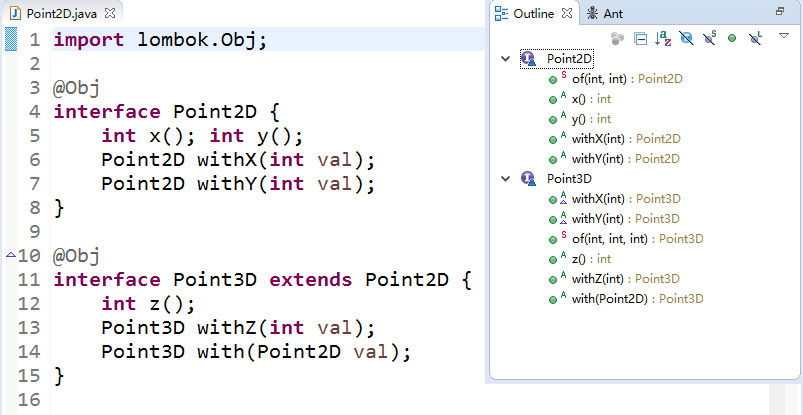
\includegraphics[width=5in]{screenshot.png}
\caption{Screenshot.}\label{screenshot_png}
\end{figure}

\haoyuan{I tried to understand the current algorithm, and did more experiments in eclipse.
Now I borrow some ideas from the current version, and give a new version of the algorithm in text. See below.

(1) I guess the function \textsf{tops} is not necessary. The first step is still
\[\textsf{mbody}(m,C_i)\in\overline{meth}\textrm{ (excluding \textbf{static} methods)}\]

(2) Assume the context is ``interface $C_0$ extends $\overline{C}$ \{$meth'$;...\}''. First handle
\[\textsf{override}(meth',\overline{meth}) \eqno{(*)}\]

(3) If $meth'\ne\none$, $(*)$ returns $meth'$ if
\[\forall meth\in\overline{meth},meth'\subtype meth\]
even if there are conflicts in $\overline{meth}$.

(4) If $meth'=\none$, we need to figure out
\[\textsf{mostSpecific}(\overline{meth})\]
and it should be the one that ``overrides'' all the others in $\overline{meth}$. It means we should not only deal with the return types of methods, but also look into the subtyping relation of interfaces. But for abstract methods, only return types are taken into consideration.
}
\end{comment}

%\text{\yanlin{shouldn't mostSpecific be: $\forall \method' \in \methods : \method \subtype
%  \method'$ ?}}

%(2) If $body_1.\textsf{returnType}=body_2.\textsf{returnType}$, \textsf{shadow} tends to return a default method. If both $body_1$ and $body_2$ are default methods, \textsf{shadow} throws an error.
%\begin{equation*}
%\begin{array}{ll}
%\textsf{shadow}(body_1, body_2)=\textsf{ERROR} & \textsf{if }body_1.\textsf{modifier}=body_2.\textsf{modifier}=\textbf{default}\\
%\textsf{shadow}(body_1, body_2)=body_1 \hspace{.1in} & \textsf{if }body_1.\textsf{modifier}=\textbf{default} \\
%\textsf{shadow}(body_1, body_2)=body_2 \hspace{.1in} & \textsf{if }body_2.\textsf{modifier}=\textbf{default} \\
%\textsf{shadow}(body_1, body_2)=body_1\textsf{ (or }body_2\textsf{)} \hspace{.1in} & \textsf{otherwise}
%\end{array}
%\end{equation*}
%
%(3) If $body_1.\textsf{returnType}<:body_2.\textsf{returnType}$, \textsf{shadow} tends to choose the one with the subtype (namely $body_1$), but only when both methods are abstract, otherwise it gives an error. The other direction $body_2.\textsf{returnType}<:body_1.\textsf{returnType}$ follows the same rule. It also gives an error if there is no subtyping relationship between two return types.
%\begin{equation*}
%\begin{array}{ll}
%\textsf{shadow}(body_1, body_2)=body_1 & \textsf{if }body_1.\textsf{modifier}=body_2.\textsf{modifier}=\emptyset\\
%& \textsf{and }body_1.\textsf{returnType}<:body_2.\textsf{returnType}\\
%\textsf{shadow}(body_1, body_2)=body_2 & \textsf{if }body_1.\textsf{modifier}=body_2.\textsf{modifier}=\emptyset\\
%& \textsf{and }body_2.\textsf{returnType}<:body_1.\textsf{returnType}\\
%\textsf{shadow}(body_1, body_2)=\textsf{ERROR} \hspace{.1in} & \textsf{otherwise}
%\end{array}
%\end{equation*}

%\subsubsection{Auxiliary function: \textsf{replace}}
%
%The \textsf{replace} function takes two same methods (with the same name and types of arguments), and gives the result of the first method overriding the second one.
%
%\begin{equation*}
%\begin{array}{ll}
%\textsf{replace}(body_1, body_2)=body_1 & \textsf{if }body_2=\emptyset\\
%\textsf{replace}(body_1, body_2)=body_2 & \textsf{if }body_1=\emptyset\\
%\textsf{replace}(body_1, body_2)=body_1 & \textsf{if }body_1.\textsf{returnType}<:body_2.\textsf{returnType}\\
%\textsf{replace}(body_1, body_2)=\textsf{ERROR} \hspace{.1in} & \textsf{otherwise}
%\end{array}
%\end{equation*}



\section{Applications and Case Studies}

This section illustrates applications and larger case studies for
Classless Java. The first application shows how a useful pattern,
using multiple inheritance and type-refinement, can be conveniently
encoded in Classless Java. The second application shows how to model
embedded DSLs based on fluent APIs. The two larger case studies, take
existing projects and refactor them into Classless Java. The first
case study shows a significant reduction in code size, while the
second case study maintains the same amount of code, but improves
modularity.

\subsection{The Expression Problem with Object Interfaces}\label{subsec:ep}

As the first application for Classless Java, we illustrate a useful
programming pattern that improves modularity and extensibility of
programs. This useful pattern is based on an existing solution to
the \emph{Expression Problem} (EP)~\cite{wadler98expression}, which is a well-known
problem about modular extensibility issues in software evolution. Recently, a
new solution~\cite{eptrivially} using only covariant type refinement was
proposed. When this solution is modeled with interfaces and default methods, it
can even provide independent extensibility~\cite{zenger05independentlyextensible}: the ability to assemble a system
from multiple, independently developed extensions. Unfortunately, the
required instantiation code makes a plain Java solution verbose and cumbersome
to use. The \mixin annotation is enough to remove the boilerplate code, making
the presented approach very appealing. Our last case study, presented
in Section~\ref{subsec:int}, is essentially a (much larger) application of this
pattern to an existing program. Here we illustrate the pattern in the
much smaller Expression Problem.

\paragraph{Initial System}
In the formulation of the EP, there is an initial system that models
arithmetic expressions with only literals and addition, and an initial
operation \texttt{eval} for expression evaluation.
As shown in Figure~\ref{fig:ep}, \texttt{Exp} is the common
super-interface with operation \texttt{eval()}
inside. Sub-interfaces \texttt{Lit} and \texttt{Add} extend interface
\texttt{Exp} with default implementations for the \texttt{eval} operation. The
number field \texttt{x} of a literal is represented as a getter method
\texttt{x()} and expression fields (\texttt{e1} and \texttt{e2}) of an addition
as getter methods \texttt{e1()} and \texttt{e2()}.

\begin{figure*}
\centering
\saveSpaceFig
\begin{tabular}{l|l}
\lstinputlisting[linerange=33-43]{../UseMixinLombok/src/casestudy/ep/TestExpression.java}% APPLY:linerange=EXPRESSION_INIT
&
\lstinputlisting[linerange=54-64]{../UseMixinLombok/src/casestudy/ep/TestExpression.java}% APPLY:linerange=EXPRESSION_PRINT
\end{tabular}
\caption{The Expression Problem (left: initial system, right: code for adding
  print operation).}\label{fig:ep}
\saveSpaceFig
\end{figure*}% \bruno{Yanlin: code is overflowing the margins. Note that
  % there are 2 spare lines that can be used on the right!}

\paragraph{Adding a New Type of Expressions}
In the OO paradigm, it is easy to add new types of expressions. For example, the
following code shows how to add subtraction.

\lstinputlisting[linerange=47-50]{../UseMixinLombok/src/casestudy/ep/TestExpression.java}% APPLY:linerange=EXPRESSION_SUB

%\marco{text under need to be improved}
\paragraph{Adding a New Operation} The difficulty of the EP in OO
languages arises from adding new operations. For example, adding a pretty printing
operation would typically change all existing code. However, a solution
%to the EP forbids this and it also forbids using casts. In other words, it should be possible
should add operations in a type-safe and modular way. This
turns out to be easily achieved with the assistance of \mixin.  The code in
Figure~\ref{fig:ep} (on the right) shows how to add the new operation \texttt{print}.
Interface \texttt{ExpP} extends \texttt{Exp} with the extra method
\texttt{print()}. Interfaces \texttt{LitP} and \texttt{AddP} are defined with
default implementations of \texttt{print()}, extending base interfaces
\texttt{Lit} and \texttt{Add}, respectively. Importantly, note that in
\texttt{AddP}, the types of ``\emph{fields}'' (i.e. the getter methods)
\texttt{e1} and \texttt{e2} are refined. If the types were not refined then
the \texttt{print()} method in \texttt{AddP} would fail to type-check.

\paragraph{Independent Extensibility}
To show that our approach supports independent extensibility, we first define a
new operation \texttt{collectLit}, which collects all
literal components in an expression. For space reasons,
we omit the definitions of the methods:

\begin{lstlisting}[]
interface ExpC extends Exp {
    List<Integer> collectLit(); }
@Obj interface LitC extends Lit, ExpC {...}
@Obj interface AddC extends Add, ExpC {
    ExpC e1(); ExpC e2(); ...}
\end{lstlisting}

\noindent Now we combine the two extensions (\texttt{print} and
\texttt{collectLit}) together:

\lstinputlisting[linerange=88-]{../UseMixinLombok/src/casestudy/ep/TestExpression.java}% APPLY:linerange=INDEPENDENT_EXTENSIBILITY


\noindent \texttt{ExpPC} is the new expression interface supporting
\texttt{print} and \texttt{collectLit} operations; \texttt{LitPC} and
\texttt{AddPC} are the extended variants. Notice that except for the routine of
\textbf{extends} clauses, no glue code is required. Return types of
\texttt{e1,e2} must be refined to \texttt{ExpPC}.

Note that the code for instantiation is automatically generated by \mixin.
Creating a simple expression of type \texttt{ExpPC} is
as simple as:
\begin{lstlisting}
ExpPC e8 = AddPC.of(LitPC.of(3), LitPC.of(4));
\end{lstlisting}
\noindent Without our approach, tedious instantiation code would need
to be defined manually.

\subsection{Embedded DSLs with Fluent Interfaces}\label{sec:dsls}
Since the style of fluent interfaces was invented in Smalltalk as method
cascading, more and more languages came to support fluent interfaces, including
JavaScript, Java, C++, D, Ruby, Scala, etc. In most languages, to create fluent
interfaces, programmers have to either hand-write everything or create a wrapper
around the original non-fluent interfaces using \textbf{this}. In Java, there
are several libraries (including jOOQ, op4j, fluflu, JaQue, etc) providing useful
fluent APIs. However most of them only provide a fixed set of predefined fluent
interfaces. Fluflu enables the creation of a fluent API and implements control
over method chaining by using Java annotations. However methods that returns
\textbf{this} are still hand-written.

The \mixin annotation can also be used to create fluent interfaces.  When
creating fluent interfaces with \mixin, there are two main advantages:
\begin{enumerate}
\item Instead of forcing programmers to hand-write code using \textbf{return
    this}, our approach with \mixin annotation removes this verbosity and
  automatically generates fluent setters.
\item The approach supports extensibility: the return types of fluent setters are
  automatically refined.
\end{enumerate}

\noindent We use embedded DSLs of two simple SQL query languages to illustrate.
The first query language \texttt{Database}  models
\texttt{select}, \texttt{from} and \texttt{where} clauses:
\lstinputlisting[linerange=6-10]{../UseMixinLombok/src/casestudy/sql/DatabaseTest.java}% APPLY:linerange=FLUENT_DATABASE
% \bruno{Wouldn't it be better to have a static method create() that calls of("","","")) and initializes all the fields? It seems awkward
% to have to use the of explicitly to initialized all fields.}

\noindent The main benefit that fluent methods give
us is the convenience of method chaining:

\lstinputlisting[linerange=33-33]{../UseMixinLombok/src/casestudy/sql/DatabaseTest.java}% APPLY:linerange=FLUENT_QUERY1

\noindent Note how all the logic for the fluent setters is automatically provided by the \mixin annotation.

\paragraph{Extending the Query Language} The previous query language can be extended with a new feature
\texttt{orderBy} which orders the result records by a field that users
specify. With \mixin programmers just need to extend the interface \texttt{Database} with new
features, and the return type of fluent setters in
\texttt{Database} is automatically refined to \texttt{ExtendedDatabase}:
\lstinputlisting[linerange=14-18]{../UseMixinLombok/src/casestudy/sql/DatabaseTest.java}% APPLY:linerange=FLUENT_DATABASE_EXT
In this way, when a query is created using \texttt{ExtendedDatabase},
all the fluent setters return the correct type, and not the old \texttt{Database} type, which would prevent calling
\texttt{orderBy}.

\lstinputlisting[linerange=39-39]{../UseMixinLombok/src/casestudy/sql/DatabaseTest.java}% APPLY:linerange=FLUENT_QUERY2

\subsection{A Maze Game}
This case study is a simplified variant of a Maze game, which is often
used~\cite{gof,bono14}
to evaluate code reuse ability related to inheritance and design
patterns. In the game, there is a player with the goal of collecting
as many coins as possible. She may enter a room with several doors to
be chosen among. This is a good example because it involves code reuse
(different kinds of doors inherit a common type, with different
features and behavior), multiple inheritance (a special kind of door
may require features from two other door types) and it also shows how
to model operations \texttt{symmetric sum}, \texttt{override} and
\texttt{alias} from trait-oriented programming. The game has been
implemented using plain Java 8 and default methods by Bono
et. al~\cite{bono14}, and the code for that implementation is
available online. We reimplemented the game using \mixin. Due to space
constraints, we omit the code here. The following table summarizes
the number of lines of code and classes/interfaces in each implementation:

\vspace{5pt}
\begin{tabular}{ccc}
\hline \rowcolor[HTML]{C0C0C0}
            & SLOC   & \# of classes/interfaces \\ \hline
Bono et al. & 335    & 14                       \\
Ours        & 199    & 11                       \\
\rowcolor[HTML]{C0C0C0}
Reduced by  & 40.6\% & 21.4\%                   \\ \hline
\end{tabular}
\vspace{5pt}

\noindent The \mixin annotation allowed us to reduce the interfaces/classes used
in Bono et al.'s implementation by 21.4\% (from 14 to 11). The
reductions were due to the replacement of instantiation classes with
generated \texttt{of} methods. The number of source lines of code 
(SLOC\footnote{Only Java code is counted, excluding comments and blank lines. })
was reduced by 40\% due to both the removal of instantiation overhead and
generation of getters/setters. %\bruno{explain why? we generate code for getters/setters?}.
To ensure a fair comparison, we used the same coding style as Bono et al.'s.

\begin{comment}
\subsection{Refactoring a Compiler}
The last case study applies our approach to a larger code base of a simple
one-pass compiler for \lstinline{C0} (a subset of \lstinline{C}). This compiler
is a handwritten, monolithic compiler used for educational purposes at Aarhus
University, Denmark\footnote{Source code available at
  http://cs.au.dk/~mis/dOvs/Czero.java}. \lstinline{C0} is restricted to
integers, several control structures and function declaration/definition and
basic I/O statements. All the code (including parsing, code generation for
various structures, error handling) is entangled in one big file. Following our
approach with \mixin, we refactored the code to several smaller interfaces
(including \lstinline{Constants}, \lstinline{MemberFields}, interfaces for
parsing different structures, etc). After the refactoring, the new code does not
reduce code as previous case studies. SLOC for original code without comments
and blank lines is 828, while ours is 830 (for fair comparison, we put all
interfaces into one file when calculating SLOC). However, the case study shows
two things: Classless Java can be applied to real code base such as compilers;
code becomes more modular without the sacrifice of code amount/simplicity.
\marco{Why we do not cite the result of the former study? the one with object algebraes
where the number of lines grown quite a while?}
\end{comment}

\subsection{Refactoring an Interpreter}\label{subsec:int}
\begin{comment}
The last case study refactors the code from an interpreter for
a Lisp-like language
\lstinline{Mumbler}\footnote{https://github.com/cesquivias/mumbler/tree/master/simple},
which is created as a tutorial for the Truffle
Framework~\cite{wurthinger2013one}.  Keeping a balance between
simplicity and useful features, \lstinline{Mumbler} contains numbers,
booleans, lists (encoding function calls and special forms such as
if-expression, lambdas, etc). In the original code base, which
consists of 626 SLOC of Java, only one operation \texttt{eval} is
supported. Extending Mumbler to support one more operation, such as a
pretty printer (making it 661 SLOC), would normally require changing the existing code base
directly.

Our refactoring applies the pattern presented in
Section~\ref{subsec:ep} to the existing Mumbler code base to improve
its modularity and extensibility. Using the refactored code base (560 SLOC) it is 
becomes possible to add new operations modularly, and to support
independent extensibility (677 SLOC). We add one more
operation \texttt{print} to both the original and the refactored code
base. In the original code base the pretty printer is added
non-modularly by modifying the existing code. In the refactored code
base the pretty printer is added modularly. 
Although the code in the refactored version is slightly increased (by 2.4\% SLOC), the
modularity is greatly increased, allowing for improved reusability and maintainability.
\end{comment}

The last case study refactors the code from an interpreter for
a Lisp-like language
\lstinline{Mumbler}\footnote{https://github.com/cesquivias/mumbler/tree/master/simple},
which is created as a tutorial for the Truffle
Framework~\cite{wurthinger2013one}.  Keeping a balance between
simplicity and useful features, \lstinline{Mumbler} contains numbers,
booleans, lists (encoding function calls and special forms such as
if-expression, lambdas, etc). In the original code base, which
consists of 626 SLOC of Java, only one operation \texttt{eval} is
supported. Extending Mumbler to support one more operation, such as a
pretty printer \texttt{print}, would normally require changing the existing code base
directly.

Our refactoring applies the pattern presented in
Section~\ref{subsec:ep} to the existing Mumbler code base to improve
its modularity and extensibility. Using the refactored code base it
becomes possible to add new operations modularly, and to support
independent extensibility. We add one more
operation \texttt{print} to both the original and the refactored code
base. In the original code base the pretty printer is added
non-modularly by modifying the existing code. In the refactored code
base the pretty printer is added modularly. 
Although the code in the refactored version is slightly increased (by 2.4\% SLOC), the
modularity is greatly increased, allowing for improved reusability and maintainability.
We list the results in the following table:

\vspace{0.5em}
{\small
\begin{tabular}{llll}
\hline
\rowcolor[HTML]{C0C0C0} 
Code               & SLOC & Code               & SLOC \\ \hline
original (\texttt{eval})         & 626  & original (\texttt{eval}+\texttt{print}) & 661  \\ 
\rowcolor[HTML]{C0C0C0}
refactored (\texttt{eval})         & 560  & refactored (\texttt{eval}+\texttt{print}) & 677  \\ \hline
\end{tabular}
}



%\section{Future work}\label{sec:futurework}
In this section we discuss potential future work.
\begin{comment}
\subsection{Encapsulation}
The biggest limitation of our approach is the inability to model visibility restrictions. For example, the absence
of support for private/protected methods in Java 8 interfaces forces all
members of interfaces to be public, including static methods. Since we use
abstract methods to encode state, our state is always all public. Still, because 
the state can only be accessed by methods, it 
is impossible for the user to know if a certain method maps directly to a field
or if it has a default implementation.  If the user wants a constructor that
does not directly maps to the fields, (as for secondary constructors in Scala)
he can simply define its own \Q@of@ method and delegate on the generated one:
\begin{lstlisting}
@Obj interface Point {  int x(); int y();
    static Point of(int val){return Point.of(val,val);} }
\end{lstlisting}
However, the generated \Q@of@ method would also be present and public.  If a
future version of Java was to support \emph{static private methods in
  interfaces} we could extend our code generation to handle also encapsulation.
  
However, interfaces as a whole can have public or 
package private (java default) visibility.

We can add a second annotation \Q!@Exposed!  that leverages on this edge: An
interface without exposed works as usual, but if any method of a public \mixin
interface is annotated with \Q!@Exposed!, we can apply a translation where a new
(package private) interface type is introduced, and the original interface become
just a facade.  For example:
\begin{lstlisting}
@Obj public interface Person{
  void name(String val);
  @Exposed default void rename(String newName){ if(/*valid name*/){ this.name(val);}}
  @Exposed String name();
  @Exposed static Person from(String val){ if(/*valid name*/){return Person.of(val);}
    throw /*invalid name*/}  }
\end{lstlisting}
becomes
\begin{lstlisting}
public interface Person{
  void rename(String newName)
  String name();
  static Person from(String val){ return Person$.from(val);} }
  
@Obj interface Person$ extends Person{//will be further expanded by @Obj
  void name(String val);
  default void rename(String newName){ if(/*valid name*/){ this.name(val);}}
  String name();
  static Person from(String val){ if(/*valid name*/){return Person$.of(val);}
    throw /*invalid name*/}  }
\end{lstlisting}

This is not a perfect solution, since
\Q@Person$@ can still be seen inside the \Q@Person@ package and heirs of
\Q@Person$@,
however it is surprising we achieve such of a good result without any language
support for privacy in interfaces.
\end{comment}

%\subsection{Qualifiers in Methods} %{Private state
\paragraph{Encapsulation} %{Private state
Since we are using Java8 to encode IB, we are unable to directly support qualifies
like private or protected. In Java 9, where private methods will be allowed in
interfaces; abstract state operations are, however, abstract methods,
so they can not be private.
Still, because the state can only be accessed by methods, it 
is impossible for the user to know if a certain method maps directly to a field
or if it has a default implementation. 

As shown by Ferruccio in [...] interfaces are enough to support privateness by a
 variation of the facade pattern:
\begin{lstlisting}
@Obj interface InternalData implements ExposedData{/*all the methods*/}//package visibility
public interface ExposedData{
  /*just the exposed interface*/
  static ExposedData of(...){return InternalData.of(...);}
  }
\end{lstlisting}

This is a safe and explicit way to list all the public interfaces and to hide all the implementation
details from outside of the package.\footnote{
Note how \Q@ExposedData.of@ do not need to map directly to the fields, and can also perform 
invariant checking.}

Using packages to as a boundary we can make all object interfaces ``with privateness''
invisible types for the rest of the program.
This preserve encapsulation, but limits inheritance:
package protected interfaces can not be seen,
thus can not be implemented from outside the package.

Using Java9 private interface methods
\footnote{Or some ugly pattern available today like public static classes with private methods}
one can define (and inherit) private behaviour; but private state inheritance in IB poses a logical challenge:
How can the heir produce initialization code for a field whose very existence is secret?

CB get around this problem in two ways: the constructor have to call a super-constructor, and
some fields can be pre-initialized.
The first idea would not provide any encapsulation benefit in IB,
since generated \Q@of@ methods expose all the field information anyway.

Pre-initialized fields could be supported by IB if we support a cache expression,
that is \Q@cache(e)@ would evaluate the expression a single time for each object, and cache the result
somewhere.\footnote{
For example, in a the compiled bytecode for objects
could have an extra field for each cached expression in its methods.
Such cache expression would be quite useful for other reasons,
including replacing involved initialization patterns.}

In this way

\begin{lstlisting}
@Obj interface MyData{
  private String f();//assuming Java9
  private MyData f(String val);
  }
\end{lstlisting}
Would be expanded into 
\begin{lstlisting}
@Obj interface MyData{
  private Box<String> _f(){return cache(Box<String>.of("hello"));}
  private String f(){return _f().val();}
  private MyData f(String val){return _f().val(val);}
  }
\end{lstlisting}

Where we could have a predefined \Q@Box@ type as\\*
\Q|@Obj interface Box<T>{ T val(); Box<T> val(T val);}|




\begin{comment}
\subsection{Class Invariants in ClassLess Java}
Since objects are created by automatically generated methods, another limitation
of our current approach is that there is no place where the user can dynamically
check for class invariants. In Java often we see code like
\begin{lstlisting}
class Point{ int x; int y;
  Point(int x; int y){this.x=x;this.y=y; assert this.checkInvariant();}
  private boolean checkInvariant(){... x>0,y>0...}
}
\end{lstlisting} 

We are considering an extension of our annotation where 
default methods with the special name \Q@checkInvariant()@ will be called inside the \Q@of@ methods.
If multiple interfaces are implemented, and more then one offers
\Q@checkInvariant()@,  a composed implementation could be automatically generated, composing by \Q@&&@ the various competing implementations.
\end{comment}
%\bruno{removed the invariants stuff; we need space, I think.}

%\subsection{Clone, toString, equals and hashCode}
\paragraph{Clone, toString, equals and hashCode}
Methods originally defined in Java class \Q@Object@, as \Q@clone@ and
\Q@toString@, can be supported by our approach with special care. If an
interface annotated with \mixin asks an implementation for \Q@clone@,
\Q@toString@, \Q@equals@ or \Q@hashCode@ we can easily generate one from the
fields.\footnote{In particular, for clone we can do automatic return type
  refinement as we do for \Q@with-@ and fluent setters. Note how this would
  solve most of the Java ugliness related to \Q@clone@ methods.}  However, if
the user wishes to provide his own implementation, since the method is also
implemented in \Q@Object@, a conflict arises. The generated code can resolve the
conflict inside \Q@of@, by implementing the method and delegating it to the user
implementation, thus

\begin{lstlisting}
@Obj interface Point { int x(); int y();
    default Point clone() { return Point.of(0,0); } } //user defined clone
\end{lstlisting} 
would expand into 

\begin{lstlisting}
interface Point { ...//as before
    public static Point of(int _x, int _y) {
        return new Point() {...
            public Point clone() { return Point.super.clone();}};} }
\end{lstlisting} 

\paragraph{A real IB language}
In this article we presented the concept of IB as a programming pattern over Java.
We do not wish to define here a complete IB language, just to show the reader IB as
a promising way to design a new oo language.
The first task is to define the set of abstract state operations.
Of course we need getters; \Q@withX@ methods seams to be pretty convenient, and they enable a
clean function programming style that would be otherwise too cumbersome.

Currently we are offering both setters and Fluent setters.
We believe be fluent setters to be sufficient; we could drop the concept of (non fluent)setters.

Manually defining abstract state methods can be verbose, we could offer a convenient syntax to 
declare get/set/with.
For example
\begin{lstlisting}
obj interface Foo{
  String bar;//== String bar(); Foo withBar(String val);
  var String beer;//also fluent setter
  }
\end{lstlisting}

We may also want to offer a compact syntax for property updaters and generalized with methods;
\begin{lstlisting}
obj interface Foo{
  updater Bar, Beer//== Foo set(Bar val); Foo set(Beer val);
  with Foo, Beer//== Foo with(Bar val); Foo with(Beer val);
  }
\end{lstlisting}
Finally, certain methods may have a specific meaning, for example
if a private method called \Q@init@ is present, it will be called after construction,
and it may be handled specially during multiple implementations, so that all relevant \Q@init@ methods are
called in some order.


\section{Related Work}\label{sec:related}
In this section we discuss related work and how it compares to Classless Java.

%\yanlin{need to discuss: whether the comments for FTJ is fair.}

%No, was not fair, I know that work, it does modular type checking, and
%more work after that they extend with more safe/modular typing things.
%also, Java8 IS a language extension on Java
%However, language extensions (including FTJ)
%have a natural drawback: the programmer has to learn new syntax. In contrast,
%our approach is completely compatible with the current Java language, so that
%programmers don't need to pay any learning cost to adapt to this new classless
%programming pattern. Another drawback which is particular for FTJ is that FTJ
%doesn't have type for traits, hence the correctness check of trait is done when
%type-checking classes. This choice makes the design of FTJ simpler but lost
%typechecking efficiency (one trait will be potentially checked multiple times if
%it is used in multiple classes).

\paragraph{Multiple Inheritance in Object Oriented Languages}
Many authors have argued in favor or against multiple inheritance.  Multiple
inheritance is very expressive, but difficult to model and implement, and can
cause difficulty (including the famous diamond (fork-join)
problem~\cite{bracha90mixin,Sak89dis}, conflicting methods, etc.) in reasoning about
programs. To conciliate the need for expressive power and simplicity, many
models have been proposed, including C++ virtual inheritance,
mixins~\cite{bracha90mixin}, traits~\cite{scharli03traits}, and hybrid models
such as CZ~\cite{malayeri2009cz}.  They provide novel programming architecture
models in the OO paradigm. In terms of restrictions set on these models, C++
virtual inheritance aims at a relative general model; the mixin model adds some
restrictions; and the trait model is the most restricted one (excluding
state, instantiation, etc).

%\paragraph{C++ Approach.}
C++ tries to provide a general solution to multiple inheritance by
virtual inheritance, dealing with the diamond problem by keeping only
one copy of the base class~\cite{ellis1990annotated}. However C++
suffers from the object initialization problem~\cite{malayeri2009cz}.
It bypasses all constructor calls to virtual superclasses, which can
potentially cause serious semantic errors. In our approach, the \mixin
annotation has full control over object initialization,
and the mechanism is transparent to users. Moreover, customized factory
methods are also allowed: if users are not satisfied with the default
generated \texttt{of} method, they can implement their own.

%\paragraph{Mixins.}
Mixins are a more restricted model than the C++ approach. Mixins allow to name
components that can be applied to various classes as reusable functionality
units. However, % they suffer from linearization: the order of mixin application
% is relevant in often subtle and undesired ways. This hinders their usability
% and the ability of resolving conflicts:
the linearization (total ordering) of
mixin inheritance cannot provide a satisfactory resolution in some cases and
restricts the flexibility of mixin composition. To fight this limitation, an
algebra of mixin operators is introduced~\cite{ancona2002calculus}, but this
raises the complexity, especially when constructors and fields
are considered~\cite{marco09FJigsaw}. Scala traits are in fact more like linearized mixins.
Scala avoids the object initialization
problem by disallowing constructor parameters, causing no ambiguity in cases
such as diamond problem. However this approach has limited expressiveness, and
suffers from all the problems of linearized mixin composition. % Other languages, such as
% Python, also use linearized mixins.
\begin{comment}
Python also offers multiple inheritance via linearized mixins. Indeed, in python any class is implicitly a mixin, and mixin composition informally expressed as\\*
\Q@ class A use B,C {...new methods...}@\\*
can be expressed in python as \\*
\Q@ class Aux: ...new methods...@\\*
\Q@ class A(B,C,Aux): pass@
\end{comment}
\noindent Java interfaces and default methods do not use
linearization: the semantics of Java \textbf{extends} clause in
interfaces is unordered and symmetric.

% However, in pure Java, there is no mechanism for creating objects in
% interfaces. Also, our approach supports proper constructor mechanism.

%\paragraph{CZ.}
Malayeri and Aldrich proposed a model CZ~\cite{malayeri2009cz} which
aims to do multiple inheritance without the diamond problem. They
divide inheritance into two separate concepts: inheritance dependency
and implementation inheritance. Using a combination of
\texttt{requires} and \texttt{extends}, a program with diamond
inheritance can be transformed to one without diamonds. Moreover,
fields and multiple inheritance can coexist. However untangling
inheritance also untangles the class structure. In CZ, not only the
number of classes, but also the class hierarchy complexity
increases. \mixin does not complicate the class structure, and state
can also coexist with multiple inheritance.

%\paragraph{Traits and Java's default methods}
Simplifying the mixins approach, traits~\cite{scharli03traits} draw a strong
line between units of reuse and object factories. Traits, as units of reusable
code, contain only methods as reusable functionality, ignoring state and state
initialization. Classes, as object factories, require functionality from
(multiple) traits. Java 8 interfaces are closely related to
traits: concrete method implementations are allowed (via the \textbf{default}
keyword) inside interfaces. The introduction of default methods opens the gate
for various flavors of multiple inheritance in Java. Traits offer an algebra
of composition operations like sum, alias and exclusion, providing explicit conflict
resolution. Former work~\cite{bono14} provides details on mimicking the trait
algebra through Java 8 interfaces.  We briefly recall the main points of their
encoding; however we propose a different representation of \textbf{exclusion}.
The first author of~\cite{bono14} agreed (via personal communication) that
our revised version for exclusion is cleaner, typesafe and more direct.
\newcommand\shortItem{\vspace{-1ex}}
\begin{itemize}
\item \textbf{Symmetric sum} can be obtained by simple multiple inheritance between interfaces.
    \begin{lstlisting}
    interface A { int x(); }    interface B { int y(); }    interface C extends A, B {}
    \end{lstlisting}
\shortItem
\item \textbf{Overriding} a conflict is obtained by specifying which super interface take precedence.
    \begin{lstlisting}
    interface A { default int m() {return 1;} }
    interface B { default int m() {return 2;} }
    interface C extends A, B { default int m() {return B.super.m();} }
    \end{lstlisting}
\shortItem
\item \textbf{Alias} is creating  a new method delegating to the existing super interface.
    \begin{lstlisting}
    interface A { default int m() {return 1;} }
    interface B extends A { default int k() {return A.super.m();} }
    \end{lstlisting}
\shortItem

\item \textbf{Exclusion}: exclusion is also supported in Java, where method declarations can hide the default methods correspondingly in the super interfaces.
    \begin{lstlisting}
    interface A { default int m() {return 1;} }
    interface B extends A { int m(); }
    \end{lstlisting}
\shortItem
\end{itemize}

There are also proposals for extending Java with traits. For
example, FeatherTrait Java (FTJ)~\cite{Liquori08ftj} extends
FJ~\cite{Igarashi01FJ} with statically-typed traits, adding trait-based
inheritance in Java.  Except for few, mostly syntactic details, their work can
be emulated with Java 8 interfaces. There are also extensions to the original
trait model, with operations (e.g. renaming~\cite{reppy2006foundation}, which breaks
structural subtyping) that default methods and interfaces cannot
model.

\emph{Traits vs Object Interfaces.}
We consider object interfaces to be an alternative to traits or mixins.  In the
trait model two concepts (traits and classes) coexist and cooperate. Some
authors~\cite{BettiniDSS13} see this as good language design fostering good
software development by helping programmers to think about the structure of
their programs.  However, other authors see the need of two concepts and the
absence of state as drawbacks of this model~\cite{malayeri2009cz}.  Object
interfaces are units of reuse, and at the same time they provide factory methods
for instantiation and support state.  Our approach promotes the use of
interfaces instead of classes, in order to rely on the modular composition
offered by interfaces. Since Java was designed for classes, a direct classless
programming style is verbose and unnatural. However, annotation-driven code
generation is enough to overcome this difficulty, and the resulting programming
style encourages modularity, composability and reusability, by keeping a strong
OO feel. In that sense, we promote object interfaces as being both units of
reusable code and object factories. Our practical experience is that, in Java,
separating the two notions leads to a lot of boilerplate code, and is quite
limiting when multiple inheritance with state is required.  Abstract state
operations avoid the key difficulties associated with multiple inheritance and
state, while still being quite expressive.  Moreover the ability to support
constructors adds expressivity, which is not available in approaches
such as Scala's traits/mixins.

%Nevertheless, we
%believe that in other languages the separation can be more practical
%than in Java, and we do not necessarily advocate that merging the two
%notions is a better approach in general.

%There are other limitations of our current approach, but they may be addressed
%in future work (see Section~\ref{sec:futurework}).


\begin{comment}
Besides, we support more features than the original trait model:
\begin{itemize}
\item We provide \texttt{of} methods for the annotated interfaces. During annotation processing time, the ``fields'' inside an interface are observed and a static method \texttt{of} is automatically injected to the interface with its arguments correspondingly. Such a method is a replacement to the constructors in original traits, making instantiation more convenient to use.
That is, in our approach there are only interfaces, our model requires a single concept, while the trait model requires traits \emph{and} classes.

\item We provide \texttt{with-} methods as auxiliary constructors. A \texttt{with-} method is generated for each field, just like record update, returning the new object with that field updated
%. A \texttt{clone} method is generated for the interface, returning a copy of the current object.
Furthermore, we do automatic return type refinement for this kind of methods. This feature is comparatively useful in big examples, making operations and behaviors more flexible.%, which we will demonstrate later.
\item We provide two options for generating setters. There are two kinds of setters which are commonly used, namely \textit{void setters} and \textit{fluent setters}. The only difference is that a fluent setter returns the object itself after setting, thus supporting a pipeline of such operations. The generation depends on which type of setter is declared in the interface by users.
\end{itemize}
\end{comment}



% \begin{enumerate}
% \item Mixins allows to name components that can be applied to various classes as
%   reusable functionality units. However, they suffer from linearization: the
%   order of mixin application is relevant in often subtitle and undesired
%   ways. constraints. This hinders their usability and their ability of resolving
%   conflicts: the linearization (total ordering) of mixin inheritance cannot
%   provide a satisfactory resolution in all cases and restricts the flexibility
%   of mixin composition.  To fight those limitations, an algebra of mixin
%   operators is introduced~\cite{ancona2002calculus}, but this raised the
%   complexity of the approach, especially when constructors and fields are
%   considered~\cite{marco09FJigsaw}.  Our approach does not have the
%   linearization problem, in that the semantics of Java \textbf{extends} clause
%   is unordered and symmetric.
% \item Simplifying the mixin algebras approach, traits draw a strong line between
%   units of reuse (traits) and object factories (classes) In this model,
%   traits~\cite{scharli03traits} units of reusable code, containing only methods
%   as reusable functionalities. Thus, no state/state initialization is
%   considered.

%   Classes act as object factories, requiring functionalities from multiple
%   traits.  Traits offers a trait algebra with operations like sum, alias and
%   exclusion, provided for explicit conflict resolution.

%   Concluding, (pure) traits do not allow state and they do not offers any reuse
%   instrument to ensure that state is coherently initialized when finally defined
%   in classes.  Traits can't be instantiated. This model requires two concepts
%   (traits and classes) to coexist and cooperate.

%   Some authors see this as good language design fostering good software
%   development by helping programmers to think about the structure of their
%   programs.  However, other authors see the need of two concepts and the absence
%   of state as drawbacks of this model. Our approach takes interfaces as units of
%   reuse, and meanwhile generates factory method for instantiation.

% \item C++ and Scala also try to provide solutions to multiple inheritance, but
%   both suffer from object initialization problems. Virtual inheritance in C++
%   provides another solution to multiple inheritance (especially the diamond
%   problem by keeping only one copy of the base class)~\cite{ellis1990annotated},
%   however suffers from object initialization problem as pointed out by Malayeri
%   et al.~\cite{malayeri2009cz}. It bypasses all constructor calls to virtual
%   superclasses, which would potentially cause serious semantic error. Scala
%   solution (very similar to linearised mixins, but misleadingly called traits in
%   the language) avoids this problem by disallowing constructor parameters,
%   causing no ambiguity in cases such as diamond problem.  This approach has
%   limited expressiveness, and suffers from all the problems of linearised mixin
%   composition.
%   Python also offers multiple inheritance via linearised mixins. Indeed in python any class is implicitly a mixin, and mixin composition informally expressed as\\*
%   \Q@ class A use B,C {...new methods...}@\\*
%   can be expressed in python as \\*
%   \Q@ class Aux: ...new methods...@\\*
%   \Q@ class A(B,C,Aux): pass@
%   Our approach not only does not involve linearised mixin problem, but also
%   support proper constructor mechanism.
% \end{enumerate}

% %\section{Comparing to traits and mixins}\label{sec:comparison}
\subsection{Multiple Inheritance in ClassLess Java}
\begin{comment}
Haoyuan

   - vs both: we do automatic return type refinement, which has useful applications
   (example: Expression Problem)

   - vs traits: we support of methods to create new objects (a replacement to constructors);
   Moreover we have the with and clone methods (we miss more applications for those). Show
   how to model the operations on traits; discuss operations that we cannot model
   (example: renaming).

   - vs mixins: we use the trait model of explicitly resolving conflicts. This is arguably
   better for reasoning.
\end{comment}

Our approach is based on forbidding the use of certain language constructs (classes), in order to rely on the modular composition offered by the rest of the language (interfaces).
Since Java was designed for classes, a direct class-less programming style is verbose and feel unnatural. However, annotation driven code generation is enough to overcome this difficulty, and
the resulting programming style encourages modularity, composability and reusability, by keeping a strong object oriented feel.
We consider our approach as an alternative to traits or mixins.

A comparison on how to to emulate the original operations on traits using Java8 can be find in\cite{bono14}. We briefly recall the main points of their encoding; however we propose a different representation of
 \textbf{exclusion}.
The author of ~\cite{bono14} agree that our revised version is cleaner, typesafe and more direct.\bruno{is this something to 
say in the paper?}

%%\newcommand\shortItem{\vspace{-1ex}}
\begin{itemize}
\begin{comment}%I shoreten up a lot after. I think this version is better but longer, and this content is just repeating bono at all.
\item \textbf{Symmetric sum}: the symmetric composition of two disjoint traits is achieved by simply implementing two interfaces in Java correspondingly, without overriding any method. The composition relies on multiple inheritance on interfaces, which is supported by Java. Below is a simple example.
    \begin{lstlisting}
    interface A { int x(); }
    interface B { int y(); }
    interface C extends A, B {}
    \end{lstlisting}
\item \textbf{Override}: the overriding operation (also known as asymmetric/preferential sum) is modelled by implementing many interfaces, while overriding some methods inside. The code below gives an example of explicitly specifying which super interface take precedence, regarding conflict on a specific method.
    \begin{lstlisting}
    interface A { default int m() {return 1;} }
    interface B { default int m() {return 2;} }
    interface C extends A, B { default int m() {return B.super.m();} }
    \end{lstlisting}
    Here the method \texttt{m()} in interface \texttt{C} simply inherits from \texttt{B.m()}.
\item \textbf{Alias}: an alias operation adds a new name to an old method when creating the new trait. In Java, we just create a new method with reference to the existing method in its super interface. See the example below, where the new method \texttt{k()} is an alias of the existing method \texttt{m()}.
    \begin{lstlisting}
    interface A { default int m() {return 1;} }
    interface B extends A { default int k() {return A.super.m();} }
    \end{lstlisting}
\end{comment}

\item \textbf{Symmetric sum} can be obtained by simple multiple inheritance between interfaces.
\shortItem
    \begin{lstlisting}
    interface A { int x(); }    interface B { int y(); }    interface C extends A, B {}
    \end{lstlisting}
\shortItem
\item \textbf{Overriding} a conflict is obtained by specifying which super interface take precedence.
\shortItem
    \begin{lstlisting}
    interface A { default int m() {return 1;} } 
    interface B { default int m() {return 2;} }
    interface C extends A, B { default int m() {return B.super.m();} }
    \end{lstlisting}
\shortItem
\item \textbf{Alias} is creating  a new method delegating to the existing super interface.
\shortItem
    \begin{lstlisting}
    interface A { default int m() {return 1;} }
    interface B extends A { default int k() {return A.super.m();} }
    \end{lstlisting}
\shortItem

\item \textbf{Exclusion}: exclusion is also supported in Java, where method declarations can hide the default methods correspondingly in the super interfaces.
\shortItem
    \begin{lstlisting}
    interface A { default int m() {return 1;} }
    interface B extends A { int m(); }
    \end{lstlisting}
\shortItem
\end{itemize}

Besides, we support more features than the original trait model:
\begin{itemize}
\item We provide \texttt{of} methods for the annotated interfaces. During annotation processing time, the ``fields'' inside an interface are observed and a static method \texttt{of} is automatically injected to the interface with its arguments correspondingly. Such a method is a replacement to the constructors in original traits, making instantiation more convenient to use.
That is, in our approach there are only interfaces, our model requires a single concept, while the trait model requires traits \emph{and} classes.

\item We provide \texttt{with-} methods as auxiliary constructors. A \texttt{with-} method is generated for each field, just like record update, returning the new object with that field updated
%. A \texttt{clone} method is generated for the interface, returning a copy of the current object.
Furthermore, we do automatic return type refinement for these kind of methods. This feature is comparatively useful in big examples, making operations and behaviours more flexible.%, which we will demonstrate later.
\item We provide two options for generating setters. There are two kind of setters which are commonly used, namely \textit{void setters} and \textit{fluent setters}. The only difference is that a fluent setter returns the object itself after setting, thus supporting a pipeline of such operations. The generation depends on which type of setter is declared in the interface by users.
\end{itemize}

These are the additional features supported by our model, conversely, there are certain operations we cannot model, such as method renaming (as in [Reppy2006]), which breaks structural subtyping.

There are other limitations of our current approach, but they may be addressed
in future work (see Section~\ref{sec:futurework}).



\paragraph{ThisType and MyType}
%\marco{ this section is unfair. There are unsolved problems with ThisType in negative positions, namely it breaks subtyping. The most common solution is to allow calling some methods only when the exact type is known. This demolishes most advantages of interfaces.}
In certain situations, object interfaces allow automatic refinement for \emph{return
types}. This is part of a bigger topic in class-based languages: expressing and
preserving type recursion and (nominal/structural) subtyping at the same time.

One famous attempt in this direction is provided by
\emph{MyType}~\cite{bruce1994paradigmatic}, representing the type of
\textbf{this}, changing its meaning along with inheritance. However when
invoking a method with MyType in a parameter position, the exact type of the
receiver must be known.  This is a big limitation in class based object oriented
programming, and is exasperated by the interface-based programming we propose: no
type is ever going to be exact since classes are not explicitly used. A recent
article~\cite{Saito2013933} lights up this topic, proposing two
new features: exact statements and nonheritable methods. Both are
related to our work: 1) any method generated inside of the \Q@of@ method is indeed
non-inheritable since there is no class name to extend from; 2) exact
statements (a form of wild-card capture on the exact run-time type) could
capture the ``exact type'' of an object even in a class-less
environment.
Admittedly, MyType greatly enhances the expressiveness and extensibility of
object-oriented programming languages. Object interfaces use covariant-return types to
simulate some uses of MyType. But our approach only works for refining
return types, whereas MyType is more general, as it also works for
parameter types. Nevertheless, as illustrated with our examples and
case studies, object interfaces are still very useful in many
practical applications.
% The addition of MyType to a language will allow easy definition of
%binary methods, methods with recursive types (i.e., the same type of the
%receiver appears in the argument or return positions of methods), etc.


\begin{comment}
\subsection{Type-Directed Translations/Syntactic Sugar}
\marco{I'm tring to merge this and the next one}
Language extensions are often implemented as syntactic sugar of the base
language. For example, Scala compiler supports XML syntax in normal Scala code
directly (after Scala ?, users need to import \texttt{scala-xml} library
manually). However, this approach is hard in terms of implementation, because it
requires extending the compiler. Also, this approach does not support combining
multiple extensions into one.

SugarJ~\cite{erdweg11sugarj} is a Java-based extensible programming language
that allows programmers to extend the base language with custom language
features by definitions in meta-DSLs (SDF, Stratego, etc).
\yanlin{Is new syntax really a ``drawback''? I think for some system, like
  SugarJ, one of purpose IS to introduce these new syntax.}  Drawbacks: new
syntax. To create the extension, programmers have to work with multiple
languages (SDF, stratego, etc) while our approach works totally in Java
environment.

We can model certain types of language extensions with annotations
only, but those extensions do not introduce new syntax: they
merely do automatic code generation.
\end{comment}

\paragraph{Meta-Programming Competes with Language Extensions}
The most obvious solution to adding features to a language is via syntactic
extensions. Syntactic extensions are often implemented as
desugarings to the base language. For example,
the Scala compiler was extended to directly support XML syntax.
However, when syntactic extensions are independently created it is hard
to combine multiple extensions into one.
SugarJ~\cite{erdweg11sugarj} is a Java-based extensible language that
aims at making the creation and composition of syntactic sugar
extensions easy, by allowing programmers to extend Java with custom
features (typically for DSLs). However SugarJ's goals are different
from language tuning: SugarJ aims at creating and composing new syntax;
whereas language tuning merely reinterprets existing syntax. It is
clear that reinterpreting existing syntax only can be limiting
for some applications. However, when language tuning is possible
it has the advantage that existing tools for the language work
out-of-the-box (since the syntax is still the same); and composition
of independently developed tunings is straightforward.

Scala-Virtualized~\cite{Rompf2012scalavirtualized} is an extension to Scala,
which allows blending shallow and deep embedding of DSLs. It redefines
some of Scala's language constructs to method calls,
which can be overridden by DSL implementer. Thus Scala-Virtualized
can also reinterpret syntax, and be seen as a form of language tuning.
However, although many Scala's language constructs are supported,
not all language constructs can be virtualized.

%These extensions are admittedly useful, however they are essentially
%creating a fork of the language, and rarely the new fork gains enough
%traction to become the main language release. % On this
% topic we mention


When the base language has a flexible enough syntax and a fast and
powerful enough reflection mechanism, we may just need to play with
operator overloading and other language tricks to discover that the
language feature we need can be expressed as a simple library in our
language. An example of this is SQLAlchemy~\cite{bayer2012sqlalchemy} in
Python, which uses operator overloading to dynamically turn normal python expressions into database queries
without requiring any syntactic extensions to Python.
Java-like languages tend to sit in the middle of two extremes:
libraries can not influence the type system, so many solutions valid
in Python or other dynamic languages are not applicable, or have the
cost of losing type-safety.

In Java-like languages compile time code generation comes at the rescue: if, for a certain feature
(\mixin in our case), it is possible to use the original language syntax to
\emph{express/describe} any specific instantiation of such feature (annotating a
class and providing getters), then we can insert in the compilation process a tool
that examines and enriches the code before compilation. No need to modify the
original source (for example we can work on temporary files).
Java is a particular
good candidate for this kind of manipulation since it already provide ways to
define and integrate such tools in its own compilation process via annotation
processing. In this way
there is no need of temporary files, and there is a well-defined way of putting
multiple extensions together.

Other languages offer even stronger support for safe code manipulation:
Template Haskell~\cite{sheard2002template}, F\# (type providers)~\footnote{http://research.microsoft.com/fsharp/} and MetaFjig (Active Libraries)~\cite{servetto2010metafjig}
all allow to execute code at compile time. They generate code that is
transparently integrated in the program that is being
generated/processed/compiled. In particular, MetaFjig offers a property called
\emph{meta-level-soundness}, ensuring by construction that library code (even if wrong or unreasonable) never generates ill-typed code. This is roughly equivalent to
\textit{Self coherence}, that we have to manually prove.
Since MetaFjig is not working on annotated classes, there is not a ``semantic with/without annotations''. Our \mixin tuning theorem does not make sense in such context.

\paragraph{Formalization of Java 8}
We provide a simple formalization for a subset of Java including
default/static interface methods and object initialization literals
(often called anonymous local inner classes).  A similar formalization
was drafted by Goetz and Field~\cite{goetz12fdefenders} to formalize
defender (default) methods in Java. In their formalization, classes
and interfaces can have only one method \Q@m()@ without arguments, so
as to simplify method overloading and renaming. Classless Java is more
general, as it supports multiple methods with arguments, it supports
static methods, and features such as multiple inheritance of
interfaces and reabstraction of default methods are also modeled.

\bruno{next comes some text that may be handy for related work}

While the motivation for default methods was to allow
interfaces to be extended over time while preserving backwards
compatibility (\emph{interface evolution}), default methods can also
emulate \emph{traits}~\cite{scharli03traits}.  \footnote{The original
  notion of traits by Scharli et al. prescribes, among other things,
  that: 1) a trait provides a set of methods that implement behavior;
  and 2) a trait does not specify any state variables, so the methods
  provided by traits do not access state variables directly. Java 8
  interfaces follow similar principles too. Indeed, a detailed
  description of how to emulate trait-oriented programming in Java 8
  can be found in the work by Bono et al.~\cite{bono14}. The Java 8
  team designing default methods, was also fully aware of that
  secondary use of interfaces, but it was not their objective to model
  traits: ``The key goal of adding default methods to Java was
  "interface evolution", not "poor man's
  traits"''~\cite{goetz13default}. As a result, they were happy to
  support the secondary use of interfaces with default methods as long
  as it did not make the implementation and language more complex.}
\marcoT{We could use Scala Traits to encode IB, but the simpler Java8
  model is a better starting point.}  \footnote{ \marco{may go in
    related work} Scala traits can declare \Q@def, val, var@ and
  \Q@lazy val@ However, while \Q@def@s can be overridden by
  \Q@val@/\Q@var@s, \Q@val@/\Q@var@s can not be overridden.\marco{we
    need to check this} A\Q@val@/\Q@var@ member is predestined to be
  instance state, and this is in sharp contrast with our model where
  the state is only a private detail of instances, and do not
  contaminate interface/trait/classes.}  \footnote{Scala traits have
  no constructor, but \Q@var@s and (\Q@lazy@) \Q@val@s can be
  ``pre-initialized''.}



\section{Interaction of Interface Methods with Interface Composition}
\bruno{I don't think this section makes alot of sense in the context 
of the new paper! I think perhaps some of this could be mentioned 
in related work.

In my opinion, instead of this section, we could have one section 
that demonstrates our implementation and its advantages.

\begin{itemize}

\item Show a diagram of how the approach works? 

\item Syntax and type system reuse; (good for error messages, for example)
\item On-the-fly AST rewriting (means no new files are created, and functionality
is immediatelly available for IDE's for example); this is better than conventional 
annotation processors.
\item Eclipse integration; code completion.
\item No integration issues in typical pre-processors; (the process is transparent; 
no need for an external tool that generates code in a first step).
\item Separate compilation (which relates to the properties?)

\end{itemize}

}
Before formalizing Classless Java and object interfaces, it is helpful
to informally discuss the behaviour of Java8
interfaces, in contrast with conventional trait models.

%We show several interesting cases
%and summarize compilation result of method composition into 3 categories:
%conflict error, accepted (both abstract) and conservative error. Meanwhile we
%also show different composition handling mechanism among traits, javac and ECJ.

\subsection{Methods in Java 8 Interfaces}
In Java 8 interfaces there are three types of methods: abstract, default, and static methods. Default and static methods were not allowed in interfaces in previous versions of Java.

\paragraph{Static methods} are handled in a very clean way: they are visible only in
  the interface in which they are explicitly defined. This means the following code
  is ill-typed.
\begin{lstlisting}
interface A0 { static int m(){return 1;} }
interface B0 extends A0 {}
... B0.m()//ill typed
\end{lstlisting}
This is different from the way static methods are handled in classes. Here
static methods have simply no interaction with interface
composition (\Q@extends@ or \Q@implements@).

\paragraph{Abstract method} composition is accepted when there exists a most specific one.
  For example, here method \texttt{Integer m()} from \texttt{B1} is visible in \Q@C1@.
\begin{lstlisting}
interface A1 { Object m(); }
interface B1 { Integer m();}
interface C1 extends A1,B1 {} //accepted
\end{lstlisting}

\paragraph{Default methods} conflict with any other default or abstract method. For
  example the following code is rejected due to method conflicts.
\begin{lstlisting}
interface A2 { default int m() {return 1;}}
interface B2 { int m(); }
interface C2 { default int m() {return 2;}}
interface D2 extends A2,B2 {} //rejected due to conflicting methods
interface E2 extends A2,C2 {} //rejected due to conflicting methods
\end{lstlisting}
Note how this is different from what happens in most trait models, where \Q@D2@
would be accepted, and the implementation in \Q@A2@ would be part of the
behavior of \Q@D2@.

\paragraph{Resolving conflicts:}
A method in the current interface wins over any method in its
super-interfaces, provided that the method
is the most specific one. This method also overrides conflict due to
inheritance. For example, the following code is accepted, but would be rejected
(see before) if the method \Q@m@ was not redefined in \texttt{D3} and
\texttt{E3}.
\begin{lstlisting}
interface D3 extends A2,B2 { int m(); } //accepted
interface E3 extends A2,C2 { default int m(){return 42;} } //accepted
\end{lstlisting}

\subsection{Classifying Outcomes of Interface Composition}
%When interfaces are composed and methods with the same name (and
%signature) exist, there are 3 possible outcomes.
%
We now try to classify possible outcomes for composition of methods with the same name (and
signature).
We will use the following (correct) declarations:
\begin{lstlisting}
interface A1 { T m(); }
interface A2 extends A1 { default T m(){ ... } }
interface A3 extends A2 { T m(); }

interface B1 { default T m(){ ... } }
interface B2 extends B1 { T m(); }
interface B3 extends B2 { default T m(){ ... } }
\end{lstlisting}

\noindent
What happens if a new interface \Q@M@ extends one \Q@A@${}_i$ and one
\Q@B@${}_j$?
% Nine representative cases are shown next:\\*
\begin{figure*}[htbp]
\centering
\begin{tabular}{|l|l|l|l|}
\hline
\textbf{M extends} & \textbf{A1}                  & \textbf{A2} & \textbf{A3} \\ \hline
\textbf{B1}        & conservative error                     & conflict error      & conservative error       \\ \hline
\textbf{B2}        & both abstract (accepted)     & conservative error       & both abstract (accepted)       \\ \hline
\textbf{B3}        & \textbf{conservative error} &conflict  error       & conservative error      \\ \hline
\end{tabular}
\end{figure*}
%We try to classify the results in the table:
\begin{itemize}
\item \textbf{conflict error} happens when the methods from both interfaces are implemented, which is also an error in most trait models.
\item \textbf{both abstract (accepted)} happens when the methods from both interfaces are abstract, which is also considered correct in all
  trait models.
\item \textbf{conservative error} happens when only one method is implemented
  (leaving another one abstract), which is different from what we would expect in
  a trait model, but is coherent with the conservative idea that a method
  defined in an interface should not silently satisfy a method in another one.
\end{itemize}

\paragraph{A bug:} During our experimentation, we found a bug in ECJ (Eclipse compiler for Java):
the case \textbf{M} extending \textbf{B3} and \textbf{A1} is accepted by
ECJ4.5.1 and rejected by javac.  By email communication with Brian Goetz
(leading Java 8 designer) we have confirmed that the expected behavior is
rejection, hence this is a bug in ECJ. This bug was also reported by
  others and is fixed in the ECJ developer branch, but not released as a stable
  version yet.



\section{Conclusion}\label{sec:conclusion}


Before Java 8, concrete methods and static methods were not allowed
to appear in interfaces.  Java 8 allows static interface methods and
introduces \emph{default methods}, which enables implementations
inside interfaces. This had an important positive consequence that
was probably overlooked: the concept of class
(in Java) is now (almost) redundant and unneeded.
We proposed a programming style, called ClassLess Java, where
truly \objectoriented programs and (reusable) libraries
can be defined and used without ever defining a single class.

However, using this programming style directly in Java is very verbose.
To avoid syntactic boilerplate
caused by Java not being originally designed to work without classes,
we introduce a new annotation, \mixin, which provides default implementations
for various methods (e.g. getters, setters, with-methods) and a
mechanism to instantiate objects. 
We leverage on annotation processing and the Lombok library, in this way
\mixin is just a normal Java library; thus our proposed style can be integrated
in any Java project.

The \mixin annotation helps programmers
to write less cumbersome code while coding in Classless Java. Indeed, 
we think the obtained gain is so high that Classless Java with the \mixin
annotation can be less cumbersome than full Java.


Class less Java is just a programming style, but is 
showing the way for a new flavour of object orientation:
We propose \interfacebased \objectoriented languages (IB),
as opposed to \classbased or \prototypebased.
In IB state is not modelled at the platonic/ideal level
but is handled excursively by instances.
This unlock useful code reuse patterns, as shown in~\ref{sec:ep}.



Interestingly, without classes there is also no subclassing. This scratches an old
  itching point in the long struggle of subtyping versus subclassing:
  according to some authors, from a software engineering perspective,
  interfaces are just a kind of classes. Others consider more
  opportune to consider interfaces as pure types. We do not know how to conciliate
  those two viewpoints and Classless Java design.
  Classless Java does not have classes purely in the Java sense.  
% Classless Java encourages coding in a more flexible way by either
% keeping a higher abstraction level (interfaces are a more abstract
% concept than classes), or relying on concrete object initialization
% (the \Q@new I(){...}@ construct).


% More generally, we identify the concept of \emph{language tuning}.
% We identify libraries that are already performing language tuning (Lombok and Cofoja), and 
% we forecast many different kinds of language tuning will emerge on suitable platforms like Java or the C\# CLR.
% We identify various kinds of safety guarantees that can be offered by language tuning, but the door is open for more flavors of safety guarantees to emerge.


\acks
We would like to thank the reviewers for their helpful comments. This work has been sponsored by the Hong Kong Research Grant Council Early Career Scheme project number 27200514.
%
% We recommend abbrvnat bibliography style.

\newpage
\clearpage
\bibliographystyle{abbrvnat}
\bibliography{paper}

% The bibliography should be embedded for final submission.

%\begin{thebibliography}{}
%\softraggedright

%\bibitem[Smith et~al.(2009)Smith, Jones]{smith02}
%P. Q. Smith, and X. Y. Jones. ...reference text...

%\end{thebibliography}





% \appendix
% \clearpage

\begin{figure*}[t]
\centering
\saveSpaceFig
\begin{grammar}
\production{
\e
}{
  \x\mid\MCall\e\m\es\mid\MCall{\C}\m\es\mid\MCall{\C\QM{.super}}\m\es\mid\x\QM=\e\QM;\e'\mid\obj
  }{expressions}\\
\production{
\obj
}{
\QM{new}\ \C\oR\cR\oC\fields\
\mh_1\oC\QM{return}\ \e_1\QM{;}\!\cC
\ldots
\mh_n\oC\QM{return}\ \e_n\QM{;}\!\cC
\cC
  }{object creation}\\
\production{\field}{\T\ \f \QM= \x\QM;}{field declaration}\\
\production{
\II
}{
 \ann\ \QM{interface}\ \C\ \QM{extends}\ \Cs\ \oC \methods\ \cC
  }{interface declaration}\\
\production{
\method
}{
 \QM{static}\ \mh\ \oC\QM{return}\ \e\QM{;}\!\cC
\mid
\QM{default}\ \mh\ \oC\QM{return}\ \e\QM{;}\cC
\mid
\mh\QM{;}
  }{method declaration}\\
\production{
\mh
}{
 \T_0\ \m\ \oR\T_1\ \x_1\ldots\T_n\ \x_n\cR
  }{method header}\\
\production{
\ann
}{
  \mixinAnn|\emptyset
  }{annotations}\\
\production{\Gamma}{
\x_1{:}\C_1\ldots\x_n{:}\C_n
}{environment}
\end{grammar}
\caption{Grammar of Classless Java}
\label{Grammar}
\end{figure*}

\begin{figure*}[t]
\centering
\saveSpaceFig
$
\begin{array}{l}

%% T-Invk
\inferrule[(T-Invk)]{
 \Gamma \vdash \e \in \C_0 \\\\
\forall i\in 1..n\ \ \Gamma \vdash \e_i \in \_<:\C_i \\\\
  \textsf{mtype}(\m,\C_0) \!=\! \C_1\ldots\C_n \!\!\to\! \C
%\textsf{mmodifier}(\m,\C) \neq \textbf{static}
 }{
 \Gamma \vdash \e\QM.\m\QM(\e_1\ldots\e_n\QM) \in \C }
\quad\quad

%%T-StaticInvk
\inferrule[(T-StaticInvk)]{
\forall i\in 1..n\  \ \Gamma \vdash \e_i\in \_<:\C_i \\\\
\textsf{mtypeS}(\m,\C_0) \!=\! \C_1\ldots\C_n \!\to\! \C
%\textsf{mmodifier}(\m,\C) = \textbf{static}
}{
\Gamma \vdash \C_0\QM.\m\QM(\e_1\ldots\e_n\QM) \in \C}
\quad\quad

%%T-SuperInvk
\inferrule[(T-SuperInvk)]{
\Gamma(\this) <: \C_0 \\\\
\forall i\in 1..n\ \ \Gamma \vdash \e_i\in \_<:\C_i \\\\
  \textsf{mtype}(\m,\C_0) \!=\! \C_1\ldots\C_n \!\!\to\! \C
%\textsf{mmodifier}(\m,\C_0) \neq \textbf{static} \\\\
}{\Gamma \vdash \C_0\QM.\QM{super}\QM.\m\QM(\e_1\ldots\e_n\QM) \in \C}


%%T-Var
\\[5ex]
\inferrule[(T-Var)]{
\Gamma(\x)=\C
}{
\Gamma \vdash \x \in\C}
\quad\quad

%%T-Obj
\inferrule[(T-Obj)]{
\forall i\in 1..k\ \ \Gamma(\x_i)\subtype\T_i\\\\
\forall i\in 1..n\ \
%\Gamma_i
\Gamma,\f_1{:}\T_1,\ldots,\f_k{:}\T_k,\,\QM{this}{:}\C,\Gamma^{\mh_i}
\vdash\e_i\in \_\subtype\C^{\mh_i}\\\\
\sigvalid(\mh_1\ldots\mh_n,I)\quad\quad\quad\quad
%\forall i\in 1..n\ \mh_i\subtype\mBody(\m^{\mh_i},\C)\\\\
\alldefined(\mh_1\ldots\mh_n,I)
%\forall\m\mbox{ such that }
%\mBody(\m,\C)=\mh\QM; \exists i\in 1..n\ \m^{\mh_i}=\m
%\forall i\in 1\ldots n\ \Gamma_i=\Gamma,\f_1{:}\T_1,\ldots,\f_k{:}\T_k,\,\QM{this}{:}\C,\Gamma^{\mh_i}
}{
\Gamma \vdash\QM{new}\ \C\oR\cR\oC\T_1\ \f_1\QM=\x_1\QM;\ldots\T_k\ \f_k\QM=\x_k\QM;\
\mh_1\oC\QM{return}\ \e_1\QM{;}\!\cC
\ldots
\mh_n\oC\QM{return}\ \e_n\QM{;}\!\cC
\cC
\in\C
}
\\[5ex]



%%T-update
\quad
\inferrule[(T-update)]{
\Gamma \vdash \e\in\_<:\Gamma(\x)\\\\
\Gamma \vdash \e'\in\C
}{
\Gamma \vdash \x\QM=\e\QM;\e'\in\C }
\quad\quad\quad

%%T-Intf
 \inferrule[(T-Intf)]{
IT(\C) = \ann\ \QM{interface}\ \C\ \QM{extends}\ \C_1\ldots\C_n \
\oC\methods\ \cC\\\\
 \forall \QM{default}\ \mh\ \oC\QM{return}\ \e\QM;\cC \in \methods,
\ \ \Gamma^{\mh},\,\QM{this}{:}\C\vdash\e\in \_\subtype\C^{\mh} \\\\
 \forall \QM{static}\ \mh\ \oC\QM{return}\ \e\QM;\cC \in \methods,
\ \ \Gamma^{\mh}\vdash\e\in \_\subtype\C^{\mh} \\\\
\dom(\C)=\dom(\C_1)\cup\ldots\cup\dom(\C_n)\cup\dom(\methods)
 }{
\C \text{ OK}
}
\end{array}$
\caption{CJ Typing}
\label{ET}
\end{figure*}

\section{Formal Semantics}\label{sec:formal}

This section presents a formalization of Classless Java, \delete{a minimal
FeatherweightJava-like calculus} which models the essence of Java
interfaces with default methods. This formalization is used \delete{in
Section~\ref{sec:translation}} to define the semantics of object interfaces.

\subsection{Syntax}

Figure~\ref{Grammar} shows the syntax of Classless Java.
The syntax formalizes a minimal
subset of Java 8, focusing on interfaces, default methods and object
creation literals.  There is no syntax for classes.
To help readability we use many metavariables to represent identifiers: $C,x,f$ and $m$; however they all map to a single set of identifiers as in Java.  Expressions
consist of conventional constructs such as variables ($\x$), method
calls ($\e\QM.\m\QM(\es)$) and static method calls
($\C\QM.\m\QM(\es)$). For simplicity the degenerate case of calling a
static method over the $\this$ receiver is not considered.  A more
interesting type of expressions is super calls
($\C\QM{.super.}\m\QM(\es)$), whose semantics is to call the (non-static) method $\m$ over the $\this$ receiver, but statically
dispatching to the version of the method as visible in the interface
$\C$. A simple form of field updates ($\x\QM=\e\QM;\e'$) is also
modeled. In the syntax of field updates $\x$ is expected to be a
field name. After updating the field $\x$ using the value of $\e$, the
expression $\e'$ is executed. To blend the statement based nature of
Java and the expression based nature of our language, we consider a
method body of the form \Q@return@ $\x\QM=\e\QM;\e'$ to represent
$\x\QM=\e\QM;\QM{return}\ \e'$ in Java.  Finally, there is an object
initialization expression from an interface $\C$, where (for
simplicity) all the fields are initialized with a variable present in
scope.
To  be fully compatible with Java, the concrete syntax for an interface
  declaration with empty supertype list  would also
  omit the \Q@extends@ keyword.
% The single
%non-Java 8 piece of syntax is the \mixin annotation, which is the only
%one interesting piece of syntax in this article.
%??? how is @Mixin not java8? in the sense that is java5?
  Following standard
practice, we consider a global Interface Table (\metaVar{IT}) mapping
from interface names $\C$ to interface declarations $\II$.

The environment $\Gamma$ is a mapping from variables to types.  As
usual, we allow a functional notation for $\Gamma$ to do variable
lookup.  Moreover, to help us define auxiliary functions, a functional
notation is also allowed for a set of methods $\methods$, using the
method name $\m$ as a key.  That is, we define $\methods(\m)=\method$
iff there is a unique $\method\in\methods$ whose name is $\m$.  For
convenience, we define $\methods(\m)=\none$ otherwise; moreover
$\m\in\dom(\methods)\ \miff\ \methods(\m)=\method$.
For simplicity, we do not model overloading, thus for an interface to be well formed its methods must be uniquely identified by their names.

\subsection{Typing}

Typing statement $\Gamma \vdash \e\in\C$ reads ``in the environment
$\Gamma$, expression $\e$ has type $\C$.''.
Before discussing the typing rules we discuss some of the used notation.
As a shortcut, we write
$\Gamma \vdash \e\in\C<:\C'$ instead of $\Gamma \vdash \e\in\C$ and
$\C<:\C'$.

We omit the definition of
the usual traditional subtyping relation between interfaces, that is the transitive and reflexive closure of the declared \Q@extends@ relation.
The auxiliary notation $\Gamma^\mh$ trivially
extracts the environment from a method header, by collecting the all types
and names of the method parameters.  The
notation $\m^\mh$ and $\C^\mh$ denotes respectively, extracting the
method name and the return type from a method header. $\mBody(\m,\C)$,
defined in Appendix~\ref{sec:auxiliary},
returns the full method declaration as seen by $\C$, that is the
method $\m$ can be declared in $\C$ or inherited from another
interface.
$\textsf{mtype}(\m,\C)$ and $\textsf{mtypeS}(\m,\C)$ return the type
signature from a method (using $\mBody(\m,\C)$ internally).
$\textsf{mtype}(\m,\C)$ is defined only for non static methods, while
$\textsf{mtypeS}(\m,\C)$ only for static ones. We use $\dom(\C)$ to
denote the set of methods that are defined for type $\C$, that is:
$\m\in\dom(\C)\ \miff \ \mBody(\m,\C)=\method$.

In Figure~\ref{ET} we show the typing rules.  We discuss the
most interesting rules, that is \rn{t-Obj} and \rn{t-Intf}. Rule
\rn{t-Obj} is the most complex typing rule. Firstly, we need to
ensure that all field initializations are type correct, by looking up the type of
each variable assigned to a field in the typing environment and verifying that such type is a
subtype of the field type. Finally, we check that all method bodies are
well-typed. To do this the environment used to check the method body
needs to be extended appropriately: we add all fields and their types;
add $\this:I$; and add the arguments (and types) of the respective
method.
Now we need to check if the object is a valid extension for that specific interface.
This can be logically divided into two steps.
First  we check that all method headers are valid
with respect to the corresponding method already present in $\C$:

\noindent$\begin{array}{l}
\InTextDef{9em}{\sigvalid(\mh_1\ldots\mh_n,I)
}{}\\
\hspace{.3in}\forall i\in 1..n\ \ \mh_i\QM;\subtype\mBody(\m^{\mh_i},\C)
\end{array}$

\noindent Here we require that for all newly declared methods, there is a method
with the same name defined in the interface $\C$, and that such method is a
supertype of the newly introduced one. We define subtyping between methods in a
general form that will also be useful later.

\noindent$\begin{array}{l}
\InTextDef{17em}{
\T\ \m\oR\T_1\x_1\ldots \T_n\x_n\cR\QM; \subtype \T' \m\oR\T_1\x_1'\ldots\T_n\x_n'\cR\QM;
}{
\T\subtype \T'
}\\
\InTextDef{15em}{\method \subtype
\QM{default}\ \mh\,\mbox{\Q@\{return \_;\}@}
}{
\method\subtype\mh\QM;
}\\
\InTextDef{15em}{\QM{default}\ \mh\,\mbox{\Q@\{return \_;\}@}\subtype\method
}{
\mh\QM;\subtype\method
}\\
\end{array}$

\noindent We allow return type specialization as introduced in Java 5. A method
header with return type $I$ is a subtype of another method header with return
type $I'$ if all parameter types are the same, and $I <: I'$. A default method
$\method_1$ is a subtype of another default method $\method_2$ iff
$\mh^{\method_1}$ is a subtype of $\mh^{\method_2}$. Secondly, we check that all
abstract methods (which need to be explicitly overridden) in the interface have
been implemented: %That is, we define a method with the same name.

\noindent$\begin{array}{l}
\InTextDef{11em}{\alldefined(\mh_1\ldots\mh_n,I)}{
\forall\m\mbox{ such that } }\\
\hspace{.3in}\mBody(\m,\C)=\mh\QM; \exists i\in 1..n\ \m^{\mh_i}=\m
\end{array}$

The rule \rn{t-intf} checks that an interface $\C$ is correctly
typed.  First we check that the body of all default and static
methods are well typed.  Then we check that $\dom(\C)$ is the same as
$\dom(\C_1)\cup\ldots\cup\dom(\C_n)\cup\dom(\methods)$.  This is not a
trivial check, since $\dom(\C)$ is defined using $\mBody$, which would be
undefined in many cases: notably if a method $\method\in\methods$ is
not compatible with some method in $\dom(\C_1)\ldots\dom(\C_n)$ or if
there are methods in any $\dom(\C_i)$ and $\dom(\C_j)$ ($i,j\in 1..n$) conflict.

\subsection{Auxiliary Definitions}\label{sec:auxiliary}

Defining \mBody{} is not trivial, and requires quite a lot of attention to the
specific model of Java interfaces, and to how it differs w.r.t. Java Class model.
$\mBody(\m,\C)$ denotes the actual method $\m$ (body included) that
interface $\C$ owns. The method can either be defined originally in $\C$ or in its supertypes, and then passed to $\C$ via inheritance.
\noindent$\begin{array}{l}
\InTextDef{15ex}{
\mBody(\m,\C_0)
}{
\override(\methods(\m),
\tops(\m,\Cs))
}\\
\InTextWith{\metaVar{IT}(\C_0) =
\ \ann\ \QM{interface}\ \C_0\ \QM{extends}\ \C_1\ldots\C_n}\\
\hspace{1.2in}\oC\methods\ \cC \mbox{ and } \C\in\Cs \mbox{ if } \C_i\subtype\C, i\in 1..n

\end{array}$

\noindent The definition of $\mBody$ reconstructs the full set of supertypes $\Cs$ and then delegates the work to two other auxiliary functions:
 $\tops(m,\Cs)$ and $\override(\method,\methods)$.

\paragraph{\tops{}} recovers from the interface table only the ``needed'' methods, that is,
the non-static ones that are not reachable by another, less specific superinterface.
Since the second parameter of \tops{} is a set, we can choose an arbitrary element to be $\C_0$.
In the definition we denote by $\Aux{originalMethod}(\m,\C)=\method$ the non-static method called $\m$ defined directly in $\C$.
%\hl{Another two functions $\super(\C_0)$ and $\get(\m,\C_0)$ are used for the definition. $\super(\C_0)$ collects the
%super interfaces of $\C_0$ recursively, and $\get(\m,\C_0)$ returns the non-static method declared in $\C_0$ with name $\m$, or $\emptyset$ otherwise.
%Finally, $\tops(\m,\C_0)$ returns the topmost methods $m$ from the super interfaces.}
Formally:

\noindent$\begin{array}{l}
\InTextDef{20ex}{
\Aux{originalMethod}(\m,\C_0)}{
\method
}\\
\InTextWith{\metaVar{IT}(\C_0) =
\ \ann\ \QM{interface}\ \C_0\ \QM{extends}\ \Cs\ \oC\methods\ \cC,}\\
\hspace{1.2in}\method\in\methods\mbox{ not static},\m=\m^\method
 \\

\InTextDef{41ex}{
\Aux{originalMethod}(\m,\C_0)\in\tops(\m,\C_0\dots\C_n)}{
 }{}\\
\tab\tab
\not\exists i\in1..n \mbox{ such that }
\Aux{originalMethod}(\m,\C_i) \mbox{ is defined }\\
\hspace{1.4in}\mbox{and } \C_i \subtype \C_0

%\\
%\InTextDef{13ex}{
%\tops(\m,\C_0)}{
%}{
%\{\ \get(\m, \C)\ |\ \C\in\super(\C_0), \get(\m, \C) \ne\emptyset,\mbox{ and }
%}\\
%\hspace{2.1in}\forall\C'\in\super(\C_0)\mbox{ and }\get(\m,\C')\ne\emptyset: \C'<:\C\Rightarrow\C'=\C\ \}\\
%\InTextDef{13ex}{
%\super(\C_0)}{
%}{
%\{\ \C'\ |\ \C'\in\Cs,\mbox{ or }\exists\C\in\Cs,\C'\in\super(\C)\ \}
%}\\
%\InTextWith{\metaVar{IT}(\C_0) =
%\ \ann\ \QM{interface}\ \C_0\ \QM{extends}\ \Cs\ \oC\methods\ \cC}\\
%\InTextDef{13ex}{
%\get(\m,\C_0)}{
%}{
%\method
%}\\
%\InTextWith{\metaVar{IT}(\C_0) =
%\ \ann\ \QM{interface}\ \C_0\ \QM{extends}\ \Cs\ \oC\methods\ \cC, \method\in\methods\mbox{ not static},\m=\m^\method}
\end{array}$


%\paragraph{\shadow{}} chooses the most specific version of a method,
%that is the unique version available, or a conflicted version from a
%set of possibilities. In this case all the conflicting defintions are returned.
%We do not model overloading, so it is an error if multiple versions are available with different parameter types. Formally:
%
%\noindent
%$\begin{array}{l}
%\InTextDef{15ex}{
%\shadow()}{\none}\\
%\InTextDef{15ex}{\shadow(\method)}{\method}\\
%\InTextDef{15ex}{\shadow(\overline{\mh\QM;})}{\Aux{mostSpecific}(\overline{\mh\QM;})}\\
%\InTextDef{15ex}{\shadow(\methods)}{\methods}\\
%\InTextWith{\mbox{ the former case not applicable} }
%%\methods\mbox{ not of the form }\overline{\mh\QM;}
%%\mbox{ and }
%%\Aux{mostSpecific}(\methods)\in\{\mh\QM;,\QM{default}\ \mh\mbox{\Q@\{return \_;\}@}\}}\\
%\end{array}$
%
\paragraph{override} models how a method in an interface can
override implementations in its superinterfaces, even in the case of
conflicts. Note how the special value $\none$ is used, and how (the 5th
case) overriding can solve a conflict.
% The notation in the last case below
%means $\method'$ is not static, and is supertype of $\method$.

\noindent$\begin{array}{l}
\InTextDef{20ex}{\override(\none,\emptyset)}{\none}\\
\InTextDef{20ex}{\override(\method,\emptyset)}{\method}\\
\InTextDef{20ex}{\override(\none,\method)}{\method}\\
\InTextDef{20ex}{\override(\none,\overline{\mh\QM;})}{\Aux{mostSpecific}(\overline{\mh\QM;})}\\
\InTextDef{20ex}{\override(\method,\methods)}{\method}\\
\InTextWith{
\forall \method' \in \methods :
%\method'\in\{\mh\QM;,\QM{default}\ \mh\,\mbox{\Q@\{return \_;\}@}, \conflicted\ \mh\QM; \},
\method\subtype\method'
}
\end{array}$

\noindent The definition $\Aux{mostSpecific}$ returns the most
specific method whose type is the subtype of all the
others.  Since method subtyping is a partial ordering,
$\Aux{mostSpecific}$ may not be defined, this in turn forces us to rely on the last clause of $\override$; otherwise
the whole \mBody{} would not be defined for that specific $\m$.
Rule \rn{t-intf} relies on this behavior.

\noindent$\begin{array}{l}
\InTextDef{18ex}{\Aux{mostSpecific}(\methods)}{\method}\\
\InTextWith{\method \in \methods\ \mand\ \forall \method' \in \methods :  \method \subtype \method'}
\end{array}$

To illustrate the mechanism of $\mBody$, we present an example. We compute $\mBody(\QM{m},\QM{D})$:
\begin{lstlisting}
interface A { Object m(); }
interface B extends A { default Object m() {return this.m();} }
interface C extends A {}
interface D extends B, C { String m(); }
\end{lstlisting}

\begin{itemize}
\item First $\{\QM{A,B,C}\}$, the full set of supertypes of $\QM{D}$ is obtained.
\item Then we compute
$\tops(\QM{m},\{\QM{A,B,C}\})= $
\Q@default Object m() {...}@,
 that is $\QM{B.m}$.
That is, we do not consider either
$\QM{C.m}$ (since $\QM{m}$ is not declared directly in $\QM{C}$, hence $\Aux{originalMethod}(\QM{m},\QM{C})$ is undefined) or $\QM{B.m}$
(that is a subtype of $\QM{A}$, thus $\QM{B.m}$ hides $\QM{A.m}$).
\item The final step computes $\override(\QM{D.m},\QM{B.m})=\QM{D.m}$,
by the last case of $\override$ we get that $\QM{D.m}$ hides $\QM{B.m}$ successfully ($\QM{String}$ is a subtype of $\QM{Object}$). Finally we get $\mBody(\QM{m},\QM{D}) = \QM{D.m}$.
\end{itemize}

% \section{What  \mixin Generates}\label{sec:translation}

\begin{figure*}[t]
\saveSpaceFig
\centering
$\begin{array}{l}
\InTextDef{16em}{[\![\mixinAnn\ \QM{interface}\ \C_0\ \QM{extends}\ \Cs\ \oC \methods\ \cC ]\!]
}{
[\![\weakAnn\ \QM{interface}\ \C_0\ \QM{extends}\ \Cs\ \oC
\methods\ \methods' \cC
]\!]}\\
\InTextWith{\methods'=\otherMethod(\C_0,\methods)}\\

\InTextDef{16em}{[\![\weakAnn\ \QM{interface}\ \C_0\ \QM{extends}\ \Cs\ \oC \methods\ \cC ]\!]
}{
\QM{interface}\ \C_0\ \QM{extends}\ \Cs\ \oC
\methods\ \ofMethod(\C_0) \cC
}\\
\InTextWith{\valid(\C_0),\QM{of}\notin\dom(\C_0) }
\end{array}$
\caption{The translation functions of $\mixinAnn$ and $\weakAnn$.}
\label{figure:translation}
\end{figure*}

\begin{figure*}[t]
\saveSpaceFig
\centering
\begin{minipage}[b]{0.5\textwidth}
$\begin{array}{l}
\InTextDef{16em}{\C_0\ \QM{with#}\m\oR \C\ \QM{_val}\cR\QM;\in
\otherMethod(\C_0,\methods)}{}\\
\hspace{.25in}\isWith(\mBody(\QM{with#}\m, \C_0), \C_0),\
\QM{with#}\m\notin\dom(\methods)\\
\InTextDef{16em}{\C_0\ \QM_\m\oR \C\ \QM{_val}\cR\QM;\in
\otherMethod(\C_0,\methods)}{}\\
\hspace{.25in}\isSetter(\mBody(\QM_\m, \C_0), \C_0),\ \QM_\m\notin\dom(\methods)\\
\InTextDef{7ex}{\valid(\C_0)}{\forall \m\in\dom(\C_0),\mbox{ if }\mh\QM; =
            \mBody(\m, \C_0),}\\
            \hspace{.24in}\mbox{ one of the following cases is satisfied:}\\
\tab\tab
\isField(\method), \isWith(\method, \C_0) \mbox{ or }
\isSetter(\method,\C_0)\\
\end{array}$
\end{minipage}
\vline
\hspace{.1in}
\begin{minipage}[b]{0.43\textwidth}
$\begin{array}{l}
\InTextDef{24ex}{\isField(\C\ \m\oR\cR\QM;)}{
\mnot\ \specialName(\m)}\\
\InTextDef{24ex}{\isWith(\C'\ \QM{with#}\m \oR \C\ \x\cR\QM;, \C_0)}{}\\
\hspace{.3in}\C_0 <: \C', \mBody(\m, \C_0) = \C\ \m\oR\cR\QM;
\ \mand\ \mnot\ \specialName(\m)\\
\InTextDef{24ex}{\isSetter(\C'\ \QM_\m \oR \C\ \x\cR\QM;, \C_0)}{}\\
\hspace{.3in}\C_0 <: \C', \mBody(\m, \C_0) = \C\ \m\oR\cR\QM;
\ \mand\ \mnot\ \specialName(\m)\\
\end{array}$
\end{minipage}
\caption{The $\otherMethod$ and $\valid$ functions (left) and
  auxiliary functions (right).}
\label{figure:valid}
\saveSpaceFig
\end{figure*}

This section gives an overview of what $\mixinAnn$ generates,
 and what formal properties are guaranteed in the translation.

We formalize syntax and typing for
 Classless Java in Appendix~\ref{sec:formal}, which models the essence of
Java interfaces with default methods.
%, including the syntax as well as
%the typing rules.
 Classless Java is just a proper subset of Java 8, so
it is easy to understand the translation presented in this section
without the syntax and typing rules of Classless Java.
Since the formalized part of Classless Java does not consider casts or \Q@instanceof@,
the \Q@with@ method is not included in the
formal translation. For the same reason \Q@void@ returning setters are
not included, since they are just a minor variation over the more
interesting fluent setters, and they would require special handling
just for the conventional \Q@void@ type.
Since our properties are about preserving typing,
we do not need to formalize Classless Java semantics to prove our statements.
\begin{figure*}[t]
\centering
\hspace{-.2in}
\begin{minipage}[b]{0.53\textwidth}
$\begin{array}{l}
\InTextDef{5em}{\ofMethod(\C_0)}{
 \QM{static}\ \C_0\ \QM{of} \oR \C_1\ \QM_\m_1\QM,\ldots \C_n\ \QM_\m_n\cR\
\QM{\{}}\\
\tab\QM{return new}\ \C_0 \oR\cR\ \QM{\{}\\
\tab\tab \C_1\ \m_1 = \QM_\m_1\QM;\ldots \C_n\ \m_n = \QM_\m_n\QM; \\
\tab\tab
\C_1\ \m_1\oR\cR\ \QM{\{return }\ \m_1\QM{;\}}\ \ldots
\C_n\ \m_n\oR\cR\ \QM{\{return }\ \m_n\QM{;\}}\\
\tab\tab\withMethod(\C_1,\m_1,\C_0,\es_1)\ldots\withMethod(\C_n,\m_n,\C_0,\es_n)\\
\tab\tab\setterMethod(\C_1,\m_1,\C_0)\ldots\setterMethod(\C_n,\m_n,\C_0)\\
%\tab\tab\cloneMethod(\C_0,\es)\\
%\tab\tab\withMethod(\C_0)\\
\tab\QM{\};\}} \\
\InTextWith{\C_1\ \m_1\QM{();},\ldots \C_n\ \m_n\QM{();} = \fieldsFunc(\C_0)}\\
\hspace{.5in}\mbox{ and }\es_i=\m_1\QM,\ldots\QM, \m_{i-1}\QM,\QM{_val,}\m_{i+1}\QM,\ldots\QM, \m_n
\end{array}$
\end{minipage}
\vline
\hspace{.2in}
\begin{minipage}[b]{0.4\textwidth}
$\begin{array}{l}
\InTextDef{16ex}{\method\in\fieldsFunc(\C_0)}{}\\
\hspace{.3in}\isField(\method)\ \mand\
\method=\mBody(m^\method,\C_0)\\
\InTextDef{10em}{\withMethod(\C,\m,\C_0,\es)}{}\\
\hspace{.2in}\C_0\ \QM{with#}\m\oR \C\ \QM{_val}\cR\ \QM{\{}
\QM{return}\ \C_0\QM{.of(}\es\QM{);\}} \\
\InTextWith{\mBody(\QM{with#}\m,\C_0) \mbox{ having the form }\mh\QM;}\\
\InTextDef{10em}{\withMethod(\C,\m,\C_0,\es)}{\emptyset\mbox{ otherwise}}\\
\InTextDef{10em}{\setterMethod(\C,\m,\C_0)}{}\\
\hspace{.2in}\C_0\ \QM_\m\oR \C\ \QM{_val}\cR\ \QM{\{}
 \m\QM{= _val;return this;\}} \\
\InTextWith{
\mBody(\QM_\m,\C_0) \mbox{ having the form }\mh\QM;}\\
\InTextDef{10em}{\setterMethod(\C,\m,\C_0)}{\emptyset\mbox{ otherwise}}\\
%\cloneMethod:&\cloneMethod(\C_0,\es)=
%\C_0\ \QM{clone()\{return}\ \C_0\QM{.of(}\es\QM{);\}} \\
%&\mbox{iff }
%\mBody(\QM{clone},\C_0) \mbox{ is of form }\mh\QM;\\
%&\cloneMethod(\C_0,\es)=\emptyset\mbox{ otherwise}\\
\end{array}$
\end{minipage}
\caption{The generated $\QM{of}$ method (left) and auxiliary functions
  (right).}
\label{figure:ofmethod}
\saveSpaceFig
\end{figure*}

\subsection{Translation}

For the purposes of the formalization, the translation is divided into
two parts for more convenient discussion on formal properties later. To this aim we introduce the annotation
$\weakAnn$. Its role is only in the translation process, hence is
not part of the Classless Java language.  $\weakAnn$ generates the
constructor method $\QM{of}$, while \mixin automatically refines the
return types and calls $\weakAnn$.

Figure~\ref{figure:translation} presents the translation. In
the first function, $\mixinAnn$
injects refined methods to interface $\C_0$. The second function, $\weakAnn$ invokes
$\ofMethod(\C_0)$ and generates the $\QM{of}$
method for $\C_0$, if such a method does not exist in its domain, and all the abstract methods are
valid for the annotation.

Figure~\ref{figure:valid} presents more details on the auxiliary
functions.
The first two points of Figure~\ref{figure:valid}
define function $\otherMethod$.
 This function generates unimplemented
 \Q@with-@ and fluent setters in the interface, where the
return types have been refined.
To determine whether a method needs to be generated,
we check if such \Q@with-@ or setter methods
require an implementation in $\C_0$, but are not declared directly in $\C_0$.
The third point gives the definition
of $\valid$:
it is valid to annotate an interface if
%To generate the \Q@of@ method, it is necessary for $\weakAnn$ to explicitly check if
all abstract methods (that is, all those
requiring an implementation) are valid.
That is, we can categorize them in a pattern that we
know how to implement (right column):
it is either a field getter (first point),
a with method (second point) or a setter (third point).
Note that we write $\QM{with#}\m$ to append $\m$ to
\QM{with}, following the camelCase rule. The first letter of $\m$
must be lower-case and is changed to upper-case upon appending. For
example \QM{with#foo}=\QM{withFoo}.  Special names $\specialName(\m)$
are \QM{with} and all identifiers of the form $\QM{with#}\m$.


Figure~\ref{figure:ofmethod}
defines the $\ofMethod$  function, which generates the static method $\QM{of}$ as an
object factory.
It detects all the field methods of $\C_0$ and use them to synthesize
its arguments.
The return statement instantiates an anonymous class which
generates the needed getters, fluent setters and with-methods.
The right column first point collects the getter methods,
the second and third point generate implementations for \texttt{with-} methods
if needed; similarly, the fourth and fifth point generate fluent setters if needed.

Some other features of $\mixinAnn$, including non-fluent
setters and the $\QM{with}$ method are not formalized here.
Appendix~\ref{subsec:otherfeatures} gives a detailed but
informal explanation of generation for those methods.


\subsection{Results}\label{subsec:results}

Classless Java provides some guarantees regarding the generated
code. Essentially, Classless Java ensures the \emph{self coherence}
and \emph{client coherence} properties informally introduced in
Section~\ref{sec:imp}. Furthermore, we can show that
\emph{if there are no type-refinements}, then \emph{heir coherence} also
holds. The result about heir coherence is possible to prove
because the translation is split into two parts. In essence heir
coherence is a property of the translation of  $\weakAnn$, but not of
\mixin.

To formally characterize the behavior of our annotation and the two levels of guarantees that we offer, we provide some notations and two theorems:
\begin{itemize}
\item We denote with $\C^{\II}$ and $m^\method$ the name of an interface and of a method.
\item An interface table
IT is OK if under such interface table, all interfaces are OK,
that is, well typed.
\item Since interface tables are just represented as sequences of interfaces we write IT = $\II$ IT' to select a specific interface in a table.
\item IT contains an heir of $\C$ if there is an interface that extends it, or a \Q@new@ that instantiates it.
\end{itemize}

\begin{thm}[@ObjOf]
If a given interface table $\II$ IT is OK
 where $\II$ has $\weakAnn$,
$\valid(\C^{\II})$  and $\QM{of}\notin\dom(\C^{\II})$,
then the interface table $[\![\II]\!]$ IT is OK.
\end{thm}

\begin{thm}[@Obj]
If a given interface table $\II$ IT is OK
 where $\II$ has $\mixinAnn$,
$\valid(\C^{\II})$  and $\QM{of}\notin\dom(\C^{\II})$, and there is no heir of $\C^{\II}$,
then the interface table $[\![\II]\!]$ IT is OK.
\end{thm}

Informally, the theorems mean that for a client program that
type-checks before the translation is applied, if the annotated type has
no subtypes and no objects of that type are created, then type safety
of the generated code is guaranteed after the successful translation.

The second
step of \mixin, namely what $\weakAnn$ does in the formalization, is
guaranteed to be type-safe for the three kinds of coherence by the $\weakAnn$ theorem.
The \mixin theorem is more interesting: since \mixin does not guarantee heir
coherence, we explicitly exclude the presence of heirs. In this way
the \mixin theorem guarantees only self and client coherence. The formal
theorem proofs are available in Appendix~\ref{sec:appendix}.

\paragraph{Type preservation}
Note that we preferred to introduce self, client and heir coherence instead of referring to conventional
type preservation theorems. The reason is
to better model how our approach behaves in a \objectoriented software ecosystem with inheritance,
where only some units may be translated/expanded.
Note inheritance's crucial influence in heir coherence.
Our formulation of client coherence allows us to discuss about intermediate
stages where only some code units are translated/expanded. Conventional
type preservation refers only to completely translated program.
Our coherence guarantees mean that developers and designers of Java libraries and frameworks
can start using IB (and our \mixin annotation) in the evolution of their products
and still retain backward compatibility with their clients.

%~\ref{subsec:lemma1},~\ref{subsec:lemma2} and~\ref{subsec:theorem}.\\

\begin{comment}
\begin{figure}[tbp]
\centering
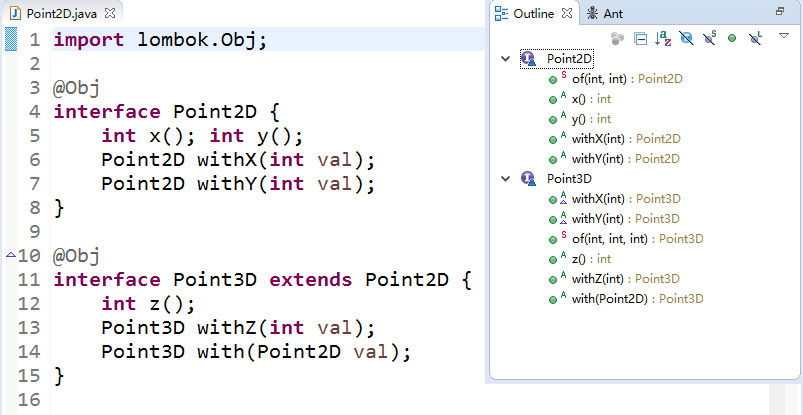
\includegraphics[width=5in]{screenshot.png}
\caption{Screenshot.}\label{screenshot_png}
\end{figure}

\haoyuan{I tried to understand the current algorithm, and did more experiments in eclipse.
Now I borrow some ideas from the current version, and give a new version of the algorithm in text. See below.

(1) I guess the function \textsf{tops} is not necessary. The first step is still
\[\textsf{mbody}(m,C_i)\in\overline{meth}\textrm{ (excluding \textbf{static} methods)}\]

(2) Assume the context is ``interface $C_0$ extends $\overline{C}$ \{$meth'$;...\}''. First handle
\[\textsf{override}(meth',\overline{meth}) \eqno{(*)}\]

(3) If $meth'\ne\none$, $(*)$ returns $meth'$ if
\[\forall meth\in\overline{meth},meth'\subtype meth\]
even if there are conflicts in $\overline{meth}$.

(4) If $meth'=\none$, we need to figure out
\[\textsf{mostSpecific}(\overline{meth})\]
and it should be the one that ``overrides'' all the others in $\overline{meth}$. It means we should not only deal with the return types of methods, but also look into the subtyping relation of interfaces. But for abstract methods, only return types are taken into consideration.
}
\end{comment}

%\text{\yanlin{shouldn't mostSpecific be: $\forall \method' \in \methods : \method \subtype
%  \method'$ ?}}

%(2) If $body_1.\textsf{returnType}=body_2.\textsf{returnType}$, \textsf{shadow} tends to return a default method. If both $body_1$ and $body_2$ are default methods, \textsf{shadow} throws an error.
%\begin{equation*}
%\begin{array}{ll}
%\textsf{shadow}(body_1, body_2)=\textsf{ERROR} & \textsf{if }body_1.\textsf{modifier}=body_2.\textsf{modifier}=\textbf{default}\\
%\textsf{shadow}(body_1, body_2)=body_1 \hspace{.1in} & \textsf{if }body_1.\textsf{modifier}=\textbf{default} \\
%\textsf{shadow}(body_1, body_2)=body_2 \hspace{.1in} & \textsf{if }body_2.\textsf{modifier}=\textbf{default} \\
%\textsf{shadow}(body_1, body_2)=body_1\textsf{ (or }body_2\textsf{)} \hspace{.1in} & \textsf{otherwise}
%\end{array}
%\end{equation*}
%
%(3) If $body_1.\textsf{returnType}<:body_2.\textsf{returnType}$, \textsf{shadow} tends to choose the one with the subtype (namely $body_1$), but only when both methods are abstract, otherwise it gives an error. The other direction $body_2.\textsf{returnType}<:body_1.\textsf{returnType}$ follows the same rule. It also gives an error if there is no subtyping relationship between two return types.
%\begin{equation*}
%\begin{array}{ll}
%\textsf{shadow}(body_1, body_2)=body_1 & \textsf{if }body_1.\textsf{modifier}=body_2.\textsf{modifier}=\emptyset\\
%& \textsf{and }body_1.\textsf{returnType}<:body_2.\textsf{returnType}\\
%\textsf{shadow}(body_1, body_2)=body_2 & \textsf{if }body_1.\textsf{modifier}=body_2.\textsf{modifier}=\emptyset\\
%& \textsf{and }body_2.\textsf{returnType}<:body_1.\textsf{returnType}\\
%\textsf{shadow}(body_1, body_2)=\textsf{ERROR} \hspace{.1in} & \textsf{otherwise}
%\end{array}
%\end{equation*}

%\subsubsection{Auxiliary function: \textsf{replace}}
%
%The \textsf{replace} function takes two same methods (with the same name and types of arguments), and gives the result of the first method overriding the second one.
%
%\begin{equation*}
%\begin{array}{ll}
%\textsf{replace}(body_1, body_2)=body_1 & \textsf{if }body_2=\emptyset\\
%\textsf{replace}(body_1, body_2)=body_2 & \textsf{if }body_1=\emptyset\\
%\textsf{replace}(body_1, body_2)=body_1 & \textsf{if }body_1.\textsf{returnType}<:body_2.\textsf{returnType}\\
%\textsf{replace}(body_1, body_2)=\textsf{ERROR} \hspace{.1in} & \textsf{otherwise}
%\end{array}
%\end{equation*}

% \section{What  \mixin Generates}\label{sec:appendixtranslation}

This section presents a formal definition for most of the generated methods by $\mixinAnn$. 

\subsection{Translation}\label{subsec:translation}

The translation functions of $\mixinAnn$ and $\weakAnn$
are presented in Figure~\ref{figure:translation}. Note that
it is necessary to explicitly check if the interface is valid
for annotation:

\noindent$\begin{array}{ll}
\InTextDef{7ex}{\valid(\C_0)}{\forall \m\in\dom(\C_0),\mbox{ if }\mh\QM; =
            \mBody(\m, \C_0),}\\
            \hspace{.24in}\mbox{ one of the following cases is satisfied:}\\
\tab\tab
\isField(\method), \isWith(\method, \C_0) \mbox{ or }
\isSetter(\method,\C_0)\\
\InTextDef{24ex}{\isField(\C\ \m\oR\cR\QM;)}{
\mnot\ \specialName(\m)}\\
\InTextDef{24ex}{\isWith(\C'\ \QM{with#}\m \oR \C\ \x\cR\QM;, \C_0)}{}\\
\hspace{.3in}\C_0 <: \C', \mBody(\m, \C_0) = \C\ \m\oR\cR\QM;
\ \mand\ \mnot\ \specialName(\m)\\
\InTextDef{24ex}{\isSetter(\C'\ \QM_\m \oR \C\ \x\cR\QM;, \C_0)}{}\\
\hspace{.3in}\C_0 <: \C', \mBody(\m, \C_0) = \C\ \m\oR\cR\QM;
\ \mand\ \mnot\ \specialName(\m)\\

%\isClone:&\isClone(\C\ \QM{clone}\oR\cR\QM;, \C_0)\tab \mif\ \C_0 <: \C \\
%\isImplemented:&\isImplemented(\method) \tab\mbox{iff }\method\mbox{ not of form }\mh\QM;
%\QM{default}\ \mh\mbox{\Q@\{return \_;\}@}) = \QM{true} \\
%&\isImplemented(\QM{static}\ \mh\mbox{\Q@\{return \_;\}@}) = \QM{true} \\
\end{array}$

\noindent That is, we can categorize all abstract methods in a pattern that we
know how to implement: it is either a field getter, a with method or a setter.

Moreover, we check that the method \Q@of@ is not already defined by the user.
In the formalization an existing definition of the \Q@of@ method is an error. However,
in the prototype (which also needs to account for overloading), the check is more complex
as it just checks that an \Q@of@ method with the same signature of the one being
generated is not already present.

We write $\QM{with#}\m$ to append $\m$ to
\QM{with}, following the camelCase rule. The first letter of $\m$
must be lower-case and is changed to upper-case upon appending. For
example \QM{with#foo}=\QM{withFoo}.  Special names $\specialName(\m)$
are \QM{with} and all identifiers of the form $\QM{with#}\m$.

\paragraph{The $\otherMethod$ function:}
$\otherMethod(\C_0,\methods)$ is defined as follows:

\noindent$\begin{array}{ll}
\InTextDef{16em}{\C_0\ \QM{with#}\m\oR \C\ \QM{_val}\cR\QM;\in
\otherMethod(\C_0,\methods)}{}\\
\hspace{.25in}\isWith(\mBody(\QM{with#}\m, \C_0), \C_0),\ 
\QM{with#}\m\notin\dom(\methods)\\
\InTextDef{16em}{\C_0\ \QM_\m\oR \C\ \QM{_val}\cR\QM;\in
\otherMethod(\C_0,\methods)}{}\\
\hspace{.25in}\isSetter(\mBody(\QM_\m, \C_0), \C_0),\ \QM_\m\notin\dom(\methods)\\
\end{array}$

\noindent The methods generated in the interface are \Q@with-@ and setters. %\Q@clone@.
%A complete formalization would also generate the \Q@with@.
The methods are generated when they are unimplemented in $\C_0$, because
the return types need to be refined.
To determine whether the methods need to be generated,
we check if such \Q@with-@ or setter methods %\Q@clone@
are required by $\C_0$, but not declared directly in $\C_0$.


\paragraph{The $\ofMethod$ function:}\label{subsec:ofmethod}
The function $\ofMethod$ generates the method \QM{of}, as an object factory. To
avoid boring digressions into well-known ways to find unique
names, %for the sake of this formalization
we assume that all methods with no parameters do not start with an underscore,
and we prefix method names with underscores to obtain valid parameter names for
\QM{of}.
\noindent$\begin{array}{l}
\InTextDef{5em}{\ofMethod(\C_0)}{
 \QM{static}\ \C_0\ \QM{of} \oR \C_1\ \QM_\m_1\QM,\ldots \C_n\ \QM_\m_n\cR\
\QM{\{}}\\
\tab\QM{return new}\ \C_0 \oR\cR\ \QM{\{}\\
\tab\tab \C_1\ \m_1 = \QM_\m_1\QM;\ldots \C_n\ \m_n = \QM_\m_n\QM; \\
\tab\tab
\C_1\ \m_1\oR\cR\ \QM{\{return }\ \m_1\QM{;\}}\ \ldots
\C_n\ \m_n\oR\cR\ \QM{\{return }\ \m_n\QM{;\}}\\
\tab\tab\withMethod(\C_1,\m_1,\C_0,\es_1)\ldots\withMethod(\C_n,\m_n,\C_0,\es_n)\\
\tab\tab\setterMethod(\C_1,\m_1,\C_0)\ldots\setterMethod(\C_n,\m_n,\C_0)\\
%\tab\tab\cloneMethod(\C_0,\es)\\
%\tab\tab\withMethod(\C_0)\\
\tab\QM{\};\}} \\
\InTextWith{\C_1\ \m_1\QM{();},\ldots \C_n\ \m_n\QM{();} = \fieldsFunc(\C_0)}\\
\hspace{.5in}\mbox{ and }\es_i=\m_1\QM,\ldots\QM, \m_{i-1}\QM,\QM{_val,}\m_{i+1}\QM,\ldots\QM, \m_n
\end{array}$

\noindent Note that, the function $\fieldsFunc(\C_0)$ denotes all the fields in the current interface:

\noindent$\begin{array}{ll}
\InTextDef{16ex}{\method\in\fieldsFunc(\C_0)}{}\\
\hspace{.3in}\isField(\method)\ \mand\
\method=\mBody(m^\method,\C_0)
\end{array}$

\noindent For methods inside the interface with the form $\C_i\ \m_i$\QM{();}
  \begin{itemize}
   \item $\m_i$ is the field name, and has type $\C_i$.
   \item $\m_i$\QM{()} is the getter and just returns the current field value.
   \item if a method \Q@with#@$\m_i()$ is required, then it is implemented by calling the \Q@of@ method using
    the current value for all the fields except for $\m_i$. Such new value is
    provided as a parameter. This corresponds to the expressions $\es_i$.
\item \QM_$\m_i$\QM($\C_i\ $\QM{ _val)} is the setter. In our prototype we use name $\m_i$, here we use the underscore to avoid modeling overloading.
%   \item similarly, for the \Q@clone@ method, \Q@of@ is called using the current value for all the fields.
   %\item To complete our generation, we need to generate setters, fluent setters and the with method.
   %\item \marco{should we just formalize setters?}
   \end{itemize}

The auxiliary functions are defined below. Note that we do not need to check if some header is a subtype of what we would generate, this is ensured by $\valid(\C_0)$.

\noindent$\begin{array}{l}
\InTextDef{10em}{\withMethod(\C,\m,\C_0,\es)}{}\\
\hspace{.2in}\C_0\ \QM{with#}\m\oR \C\ \QM{_val}\cR\ \QM{\{}
\QM{return}\ \C_0\QM{.of(}\es\QM{);\}} \\
\InTextWith{\mBody(\QM{with#}\m,\C_0) \mbox{ having the form }\mh\QM;}\\
\InTextDef{10em}{\withMethod(\C,\m,\C_0,\es)}{\emptyset\mbox{ otherwise}}\\
\InTextDef{10em}{\setterMethod(\C,\m,\C_0)}{}\\
\hspace{.2in}\C_0\ \QM_\m\oR \C\ \QM{_val}\cR\ \QM{\{}
 \m\QM{= _val;return this;\}} \\
\InTextWith{
\mBody(\QM_\m,\C_0) \mbox{ having the form }\mh\QM;}\\
\InTextDef{10em}{\setterMethod(\C,\m,\C_0)}{\emptyset\mbox{ otherwise}}\\
%\cloneMethod:&\cloneMethod(\C_0,\es)=
%\C_0\ \QM{clone()\{return}\ \C_0\QM{.of(}\es\QM{);\}} \\
%&\mbox{iff }
%\mBody(\QM{clone},\C_0) \mbox{ is of form }\mh\QM;\\
%&\cloneMethod(\C_0,\es)=\emptyset\mbox{ otherwise}\\
\end{array}$

\subsection{Other Features}\label{subsec:otherfeatures}

We do not formally model non-fluent setters and the \Q@with@ method.
An informal explanation of how those methods are generated is given next:
\begin{itemize}
\item For methods inside the interface with the form \Q@void @$\m$\QM($\C\ \x$\QM{);}:
  \begin{itemize}
    \item Check if method $\C\ \m$\Q@();@ exists. If not, generate error (that
      is, $\valid(\C_0)$ is false).
    \item Generate the implemented setter method inside \Q@of@:\\*
      \Q@public void @$\m$\Q@(@$\C$\Q@ _val) { @$\m$\Q@=_val;}@\\*
      There is no need to refine the return type for non-fluent setters, thus we
      do not need to generate the method header in the interface body itself.
    \end{itemize}
\item For methods with the form $\C'\ $\QM{with(}$\C\ \x$\QM{);}:
  \begin{itemize}
   \item $\C$ must be an interface type (no classes or primitive types).
    \item As before, check that $\C'$ is a supertype of the current interface type $\C_0$.
    \item Generate implemented \Q@with@ method inside \Q@of@:\\*
           \Q@public @$\C_0\ $\Q@with(@$\C$\Q@ _val) { @\\*
           \Q@  if(_val instanceof @$\C_0$\Q@){return (@$\C_0$\Q@)_val;}@\\*
${}_{}$\Q@  return @$\C_0$\Q@.of(@$\e_1\ldots\e_n$\Q@);}@\\*
 with $\e_i=$\Q@_val.@$\m_i$\Q@()@ if $\C$ has a $\m_i$\Q@()@ method where
 $\m_1\ldots\m_n$ are fields of $\C_0$; otherwise $\e_i=\m_i$.
    \item If needed, as for \Q@with-@ and setters, generate the method headers with refined return types in the interface.
 \end{itemize}

%\item For methods with the form $\C'\ \m$\QM($\C\ \x$\QM{);}:
 % \begin{itemize}
  %  \item As for before, check if exist method $\C\ \m$\Q@();@. Also, check that $\C'$ is a supertype of the current interface type $\C_0$.
   % \item Generate implemented setter method inside \Q@of@:\\*
    %       \Q@public @$\C_0\ \m$\Q@(@$\C$\Q@ _val) { @$\m$\Q@=_val; return this;}@
   % \item If needed, as for \Q@with-@ and clone, generate the method header with refined return type in the interface.
 % \end{itemize}
\end{itemize}


% \newpage

\section{Appendix}\label{sec:appendix}

\subsection{LEMMA 1 and Proof}\label{subsec:lemma1}

\textbf{LEMMA 1. }
For any expression $e$ under an interface table $\II$ IT where $\Gamma\vdash e\in\C^\II$, $\II$ has \textbf{@ObjWeak} annotation and $[\![\II]\!] = \II'$, then under the interface table $\II'$ IT, $\Gamma\vdash e\in\C^\II$.
\begin{proof}
By induction on the typing rules: by the grammar shown in Figure~\ref{Grammar}, there are 6 cases for an arbitrary expression $e$:
\begin{itemize}
\item Variables are typed in the same exact way.
\item Field update. The type preservation is ensured by induction.
\item A method call (normal, static or super). The corresponding method declaration won't be ``removed'' by the translation, also the types remain unchanged. The only work \textbf{@ObjWeak} does is adding a static method $\QM{of}$ to the interface, however, a pre-condition of the translation is $\QM{of}\notin\dom(\C^\II)$, so adding $\QM{of}$ method has no way to affect any formerly well typed method call.
\item An object creation. Adding the $\QM{of}$ method doesn't introduce unimplemented methods to an interface, moreover, the static method is not inheritable, hence after translation such an object creation still type checks and has the right type by induction.
\end{itemize}
\end{proof}
\textbf{LEMMA 1b. }
For any expression $e$ under an interface table $\II$ IT where there is no heir of $\C^\II$,  $\Gamma\vdash e\in\C^\II$, $\II$ has \mixin annotation and $[\![\II]\!] = \II'$, then under the interface table $\II'$ IT, $\Gamma\vdash e\in\_<:\C^\II$.
\begin{proof}
The proof follows the same scheme of the Lemma1, but for the case of method call the return type may be refined with a subtype. This is still ok since we require $\_<:\C^\II$. On the other side, this weaker result still allows the application on the method call typing rules, since in the premises the types of the actual parameter are required to be a subtype of the formal one.
\end{proof}
\subsection{LEMMA 2 and Proof}\label{subsec:lemma2}

\textbf{LEMMA 2. }
If $\II$ has \textbf{@ObjWeak} annotation and $\C^{\II}$ OK in $\II$ IT, then $[\![\II]\!]$ OK in $[\![\II]\!]$ IT.
\begin{proof}

By the rule \rn{t-Intf} in Figure~\ref{ET}, we divide the proof into two parts.

\noindent\textbf{Part I.} For each default or static method in the domain of $[\![\C^\II]\!]$, the type of the return value is compatible with the method's return type.

Since $\II$ OK, and by \textbf{LEMMA 1}, all the existing default and static methods are well typed in $[\![\II]\!]$, except for the new method \QM{of}. It suffices to prove that it still holds for $\ofMethod(\C)$.


By the definition of $\ofMethod(\C)$, the return value is an object $$\QM{return new}\ \C^\II \oR\cR\ \QM{\{}...\ \QM{\}}$$
To prove it is of type $\C^\II$, we use the typing rule \rn{t-Obj}.

\begin{itemize}
\item All field initializations are type correct. By the definition of $\ofMethod(\C^\II)$ in Section~\ref{subsec:ofmethod}, the fields $m_1,\ldots,m_n$ are initialized by $\QM{of}$'s arguments, and types are compatible.
\item All method bodies are well-typed.
    \begin{itemize}
    \item Typing of the $i$-th getter $m_i$. \[\Gamma, m_i:\C_i, \QM{this}:\C^\II \vdash m_i\in \C_i\]
        We know that $\C_i=\C^{\mh_i}$ since the $i$-th getter has its return type the same as the corresponding field $m_i$.
    \item Typing of the \QM{with-} method of an arbitrary field $m_i$. By Section~\ref{subsec:ofmethod}, if the \QM{with-} method of $m_i$ is well-defined, it has the form \[\C^\II\ \QM{with#}\m_i\oR \C_i\ \QM{_val}\cR\ \QM{\{}\QM{return}\ \C^\II\QM{.of(}\es_i\QM{);\}}\]
        $\es_i$ is obtained by replacing $m_i$ with $\QM{_val}$ in the list of fields, and since they have the same type $\C_i$, the arguments $\es_i$ are compatible with $\C^\II.\QM{of}$ method. Hence \[\Gamma, m_1:\C_1\ldots m_n:\C_n, \QM{this}:\C^\II,\ \QM{_val} : \C_i \vdash \C^\II\QM{.of}\oR\es_i\cR\in \C^\II\]
        We know that $\C^\II=\C^{\mh_i}$ by the return type of $\QM{with#}\m_i$ shown as above.
    \item Typing of the $i$-th setter \QM_$m_i$. If the \QM_$m_i$ method is well-defined, it has the form
        \[\C^\II\ \QM_\m_i\oR \C_i\ \QM{_val}\cR\ \QM{\{} \m_i\QM{= _val;return this;\}}\]
        By \rn{t-Update}, the assignment ``$\m_i\QM{= _val;}$'' is correct since $\m_i$ and $\QM{_val}$ have the same type $I_i$, and the return type is decided by \QM{this}. \[\Gamma, \QM{this}:\C^\II,\ \QM{_val} : \C_i \vdash\QM{this}\in \C^\II\]
        We know that $\C^\II=\C^{\mh_i}$ by the return type of $\QM_\m_i$ shown as above.\\
        \haoyuan{Can we write $\Gamma, \QM{this}:\C^\II,\ \QM{_val} : \C_i, \C^{\mh_i} = \C^\II \vdash\QM{this}\in \C^\II = \C^{\mh_i}$?}\\
        \haoyuan{Can we write $\QM{\{} \m_i\QM{= _val;return this;\}} \in \C^\II$?}
      \marco{Not without defining what that would mean. Do we need to? it seams good as it is now...}
    \end{itemize}
\item All method headers are valid with respect to the domain of $\C^\II$. Namely $$\sigvalid(\mh_1\ldots\mh_n,I)$$
    For convenience, we use ``$\method$ in $\ofMethod(\C^\II)$'' to denote that $\method$ is one of the implemented methods in the return expression of $\ofMethod(\C^\II)$, namely \Q@new@ $\C^\II$\Q@(){...}@.
    \begin{itemize}
    \item For the $i$-th getter $m_i$,
        \begin{align*}
        &\C_i\ \m_i\oR\cR\ \QM{\{...\}}\mbox{ in }\ofMethod(\C^\II)\\
        \mimply\hspace{.2in}& \C_i\ \m_i\oR\cR\QM; \in \fieldsFunc(\C^\II)\\
        \mimply\hspace{.2in}& \C_i\ \m_i\oR\cR\QM; = \mBody(m_i,\C^\II)\\
        \mimply\hspace{.2in}& \C_i\ \m_i\oR\cR\QM; <: \mBody(m_i,\C^\II)
        \end{align*}
    \item For the $\QM{with#}\m_i$ method,
        \begin{align*}
        &\C^\II\ \QM{with#}\m_i\oR \C_i\ \QM{_val}\cR\ \QM{\{...\}}\mbox{ in }\ofMethod(\C^\II)\\
        \mimply\hspace{.2in}& \mBody(\QM{with#}\m_i,\C^\II) \mbox{ is of form }\mh\QM;\\
        \mbox{with}\hspace{.2in}& \valid(\C^\II)\\
        \mimply\hspace{.2in}& \isWith(\mBody(\QM{with#}\m_i,\C^\II),\C^\II)\\
        \mimply\hspace{.2in}& \C^\II\ \QM{with#}\m_i\oR \C_i\ \QM{_val}\cR\QM; <: \mBody(\QM{with#}\m_i,\C^\II)
        \end{align*}
    \item For the $i$-th setter $\QM_\m_i$,
        \begin{align*}
        &\C^\II\ \QM_\m_i\oR \C_i\ \QM{_val}\cR\ \QM{\{...\}}\mbox{ in }\ofMethod(\C^\II)\\
        \mimply\hspace{.2in}& \mBody(\QM_\m_i,\C^\II) \mbox{ is of form }\mh\QM;\\
        \mbox{with}\hspace{.2in}& \valid(\C^\II)\\
        \mimply\hspace{.2in}& \isSetter(\mBody(\QM_\m_i,\C^\II),\C^\II)\\
        \mimply\hspace{.2in}& \C^\II\ \QM_\m_i\oR \C_i\ \QM{_val}\cR\QM; <: \mBody(\QM_\m_i,\C^\II)
        \end{align*}
    \end{itemize}
\item All abstract methods in the domain of $\C^\II$ have been implemented. Namely $$\alldefined(\mh_1\ldots\mh_n,I)$$
    Here we simply refer to $\valid(\C^\II)$, since it guarantees each abstract method to satisfy $\isField$, $\isWith$ or $\isSetter$. But that object includes all implementations for those cases. A getter $m_i$ is generated if it satisfies $\isField$; a \Q@with-@ method is generated for the case $\isWith$, by the definition of $\withMethod$; a setter for $\isSetter$, similarly, by the definition of $\setterMethod$. Hence it is of type $\C^\II$ by \rn{t-Obj}.
\end{itemize}

\noindent\textbf{Part II.} Next we check that in $[\![\II]\!]$, $$\dom([\![\II]\!])=\dom(\C_1)\cup\ldots\cup\dom(\C_n)\cup\dom(\methods)\cup\dom(\method')$$

Since $\II$ OK, we have $\dom(\II)=\dom(\C_1)\cup\ldots\cup\dom(\C_n)\cup\dom(\methods)$, and hence it is equivalent to prove $$\dom([\![\II]\!])=\dom(\C^\II)\cup\dom(\method')$$
This is obvious since a pre-condition of the translation is $\QM{of}\notin\dom(\C^\II)$, so $\method'$ doesn't overlap with $\dom(\C^\II)$. The definition of $\dom$ is based on $\mBody$, and here the new domain $\dom([\![\II]\!])$ is only an extension to $\dom(\C)$ with the \QM{of} method, namely $\method'$. Also note that after translation, there are still no methods with conflicted names, since the \QM{of} method was previously not in the domain, hence $[\![\II]\!]$ is well-formed, which finishes our proof.
\end{proof}

\textbf{LEMMA 2b. }
If $\II$ has \mixin annotation $\C^{\II}$ OK in $\II$ IT
and there is no heir of $\C^\II$, then $[\![\II]\!]$ OK in $[\![\II]\!]$ IT.
\begin{proof}
\noindent\textbf{Part I.} Similarly to what already argued for Lemma2, 
since $\II$ OK, and by \textbf{LEMMA 1b}, all the existing default and static methods are well typed in $[\![\II]\!]$,IT.
The translation function delegate its work to \Q!@ObjWeak! in such way that we can refer to 
Lemma2  to complete this part. Note that all the methods that are added (directly) by \mixin are abstract, and thus there is no body to typecheck.


\noindent\textbf{Part II.}
Similar to what already argued for Lemma2, but we need to notice that the the newly added methods are valid refinements for already present methods in $\dom(\C^\II)$ before the translation.
Thus by last clause of the definition of $\override(\_)$, $\mBody(\_)$ is defined on the same method names.
\end{proof}


\subsection{THEOREM and Proof}\label{subsec:theorem}
 
\noindent\textbf{THEOREM }\Q!@ObjWeak!\\*
If a given interface table $\II$ IT is OK\\*
 where $\II$ has \Q!@ObjWeak!, 
$\valid(\C^{\II})$  and $\QM{of}\notin\dom(\C^{\II})$,\\*
then the interface table $[\![\II]\!]$ IT is OK.

\begin{proof}
\textbf{LEMMA 2} already proves that $[\![\II]\!]$ is OK. On the other hand, for any $\II'\in $ IT$\setminus\II$, by \textbf{LEMMA 1}, we know that all its methods
are still well-typed, and the generated code in translation of \textbf{@ObjWeak} is only a static method \QM{of}, which has no way to affect the domain
of $\II'$, so after translation rule \rn{t-Intf} can still be applied, which finishes our proof.
\end{proof}

\noindent\textbf{THEOREM }\Q!@Obj!\\*
If a given interface table $\II$ IT is OK\\*
 where $\II$ has \Q!@Obj!, 
$\valid(\C^{\II})$  and $\QM{of}\notin\dom(\C^{\II})$, and there is no heir of $\C^{\II}$,\\*
then the interface table $[\![\II]\!]$ IT is OK.


\begin{proof}
Similar to what already argued for \textbf{THEOREM }\Q!@ObjWeak!
we can apply \textbf{LEMMA 2b} and \textbf{LEMMA 1b}. Then we finsh by \textbf{THEOREM }\Q!@ObjWeak!.
\end{proof}



\end{document}
